% !TeX root = ../main.tex

% Slides
\section{Visão geral}
\begin{frame}[c]{Visão geral}
    \begin{columns}[c]
        \vspace*{-0.5cm}
        \begin{column}{0.48\linewidth}
            \begin{splusbox}{}
                \begin{itemize}
                    \item Introdução
                    \begin{itemize}
                        \item Contexto cosmológico
                        \item Estrutura em larga escala
                        \item Redshifts espectroscópicos e fotométricos
                    \end{itemize}
                    \item Objetivo
                    \item Dados
                    \begin{itemize}
                        \item Fotométricos e espectroscópicos
                        \item Pré-processamento
                        \item Pesos por objeto
                    \end{itemize}
                \end{itemize}
            \end{splusbox}
        \end{column}
        %
        \begin{column}{0.48\linewidth}
            \begin{splusbox}{}
                \begin{itemize}
                    \item Metodologia
                    \begin{itemize}
                        \item Redes neurais
                        \item Redes neurais Bayesianas
                        \item Redes de mistura de densidades
                    \end{itemize}
                    \item Resultados
                    \begin{itemize}
                        \item Redshifts fotométricos
                        \item Funções de densidade de probabilidade
                        \item Estrutura em larga escala
                    \end{itemize}
                    \item Conclusões e perspectivas
                \end{itemize}
            \end{splusbox}
        \end{column}
    \end{columns}

 \end{frame}

\section{Introdução}
\begin{frame}[c]{O contexto cosmológico}
    \begin{splusbox}{}
        Estudar a formação e evolução da estrutura em larga escala (LSS) é fundamental para entender o Universo em que vivemos. A partir dela podemos ter insights sobre:
        \begin{itemize}
            \item Matéria escura
            \item Energia escura
            \item Evolução cósmica
            \item Formação e evolução de galáxias
            \item Física a nível fundamental
        \end{itemize}
    \end{splusbox}
\end{frame}

% \begin{frame}[c]{Estrutura em larga escala}
%     A teia cósmica, ou a LSS, é formada por diferentes componentes. Cada componente apresenta caracteristicas e possui papéis diferentes na evolução do Universo como um todo.

%     \begin{figure}
%         \centering
%         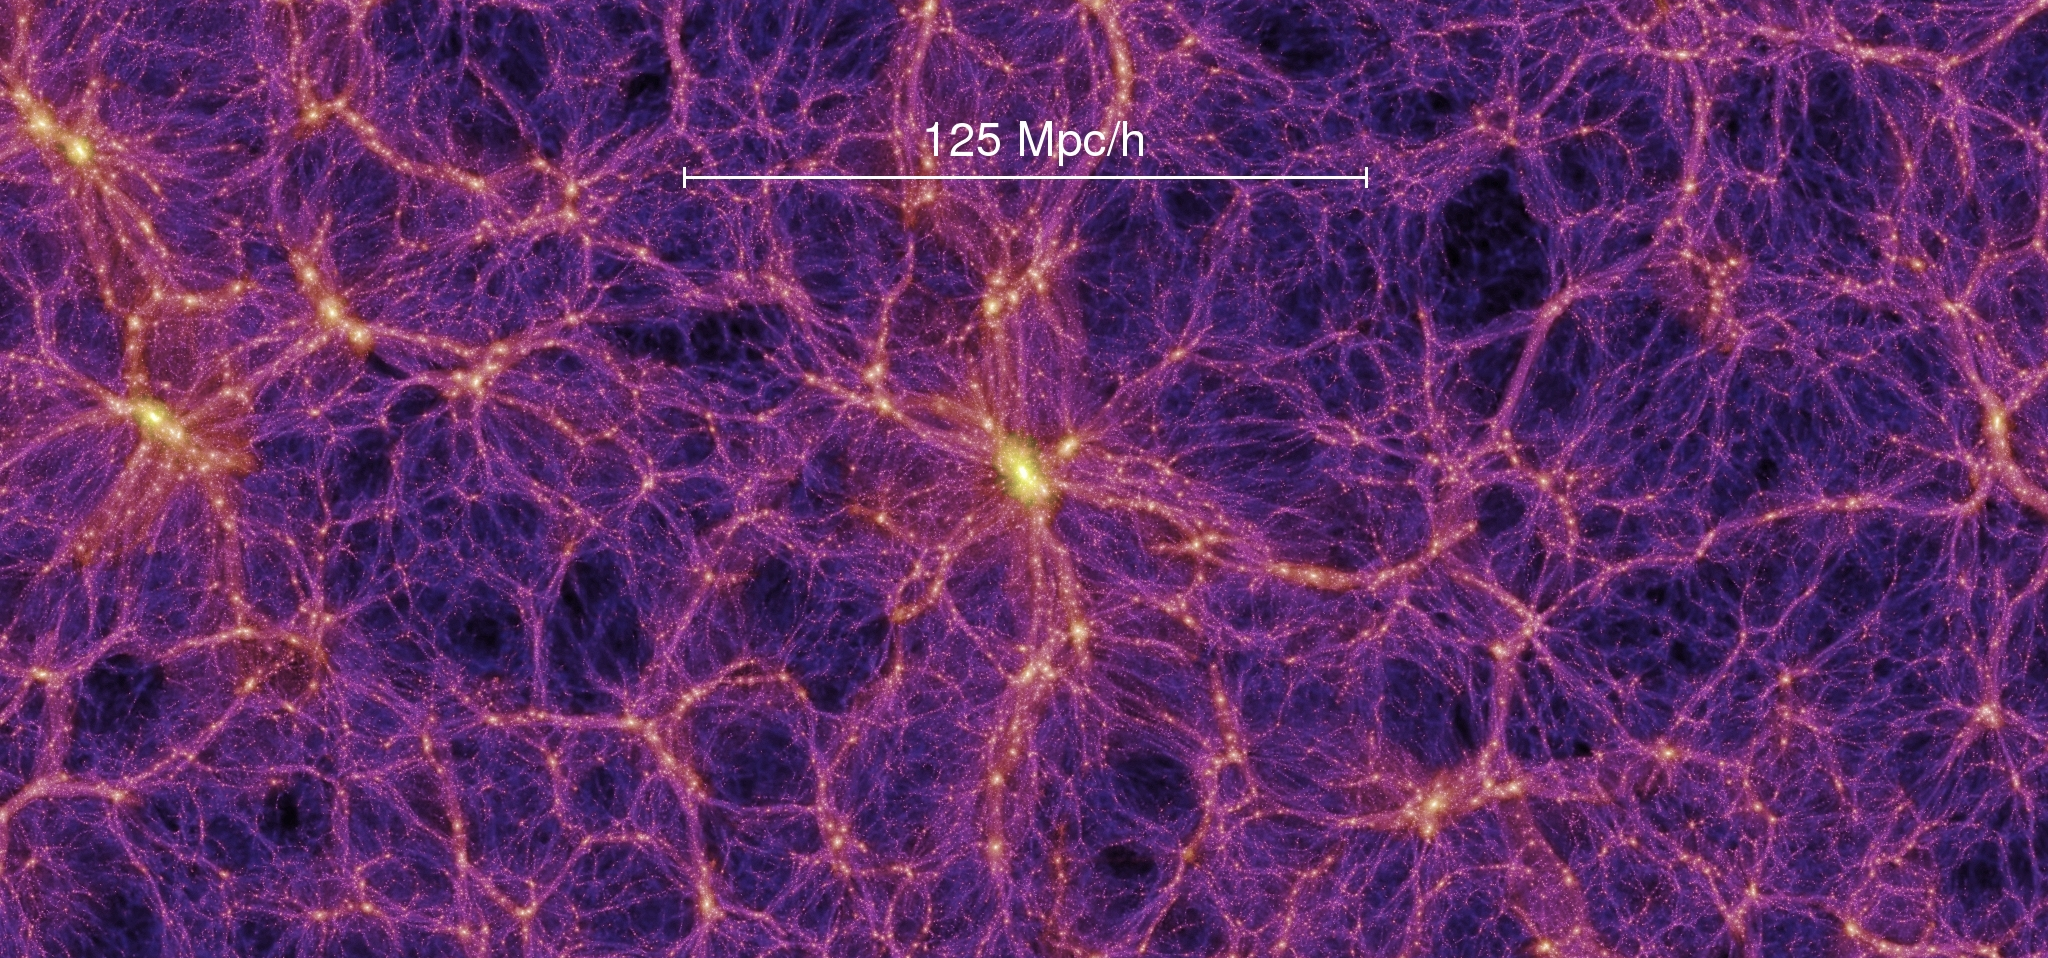
\includegraphics[height=5cm]{script/images/millenium.png}
%         \caption{Adaptado de \url{https://wwwmpa.mpa-garching.mpg.de/galform/virgo/millennium/}.}
%     \end{figure}

%     % \begin{columns}
%     %     \begin{column}{0.32\linewidth}
%     %         \begin{splusbox}{Filamentos}
                
%     %         \end{splusbox}
%     %     \end{column}
%     %     %
%     %     \begin{column}{0.32\linewidth}
%     %         \begin{splusbox}{Aglomerados}
                
%     %         \end{splusbox}
%     %     \end{column}
%     %     %
%     %     \begin{column}{0.32\linewidth}
%     %         \begin{splusbox}{Vazios}
                
%     %         \end{splusbox}
%     %     \end{column}
%     % \end{columns}
% \end{frame}

% \begin{frame}[c]{Estrutura em larga escala}
%     \begin{figure}
%         \centering
%         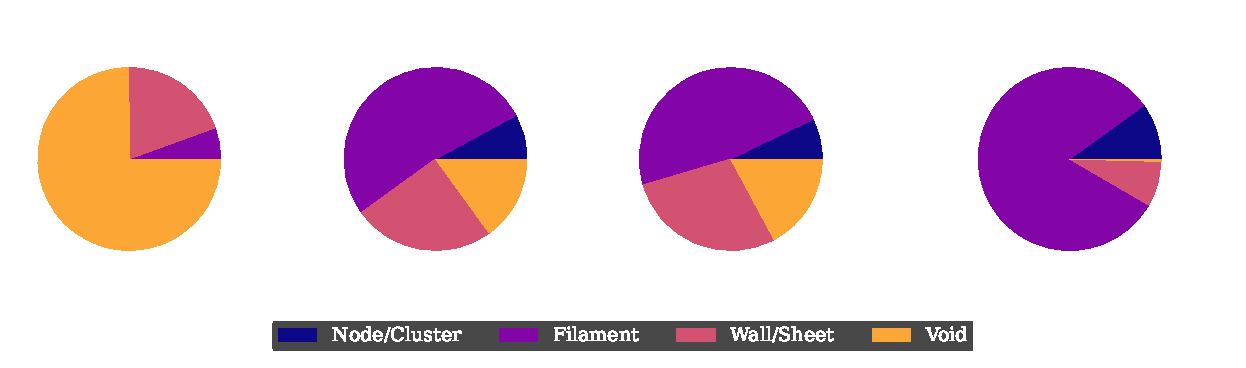
\includegraphics[width=\linewidth]{script/images/lss_distribution.pdf}
%         \caption{Adaptado de: Ganeshaiah Veena et al. (2019).}
%     \end{figure}
% \end{frame}

% \begin{frame}[c]{Estrutura em larga escala}
%     \begin{columns}[c]
%         \begin{column}{0.56\textwidth}
%             \begin{figure}
%                 \centering
%                 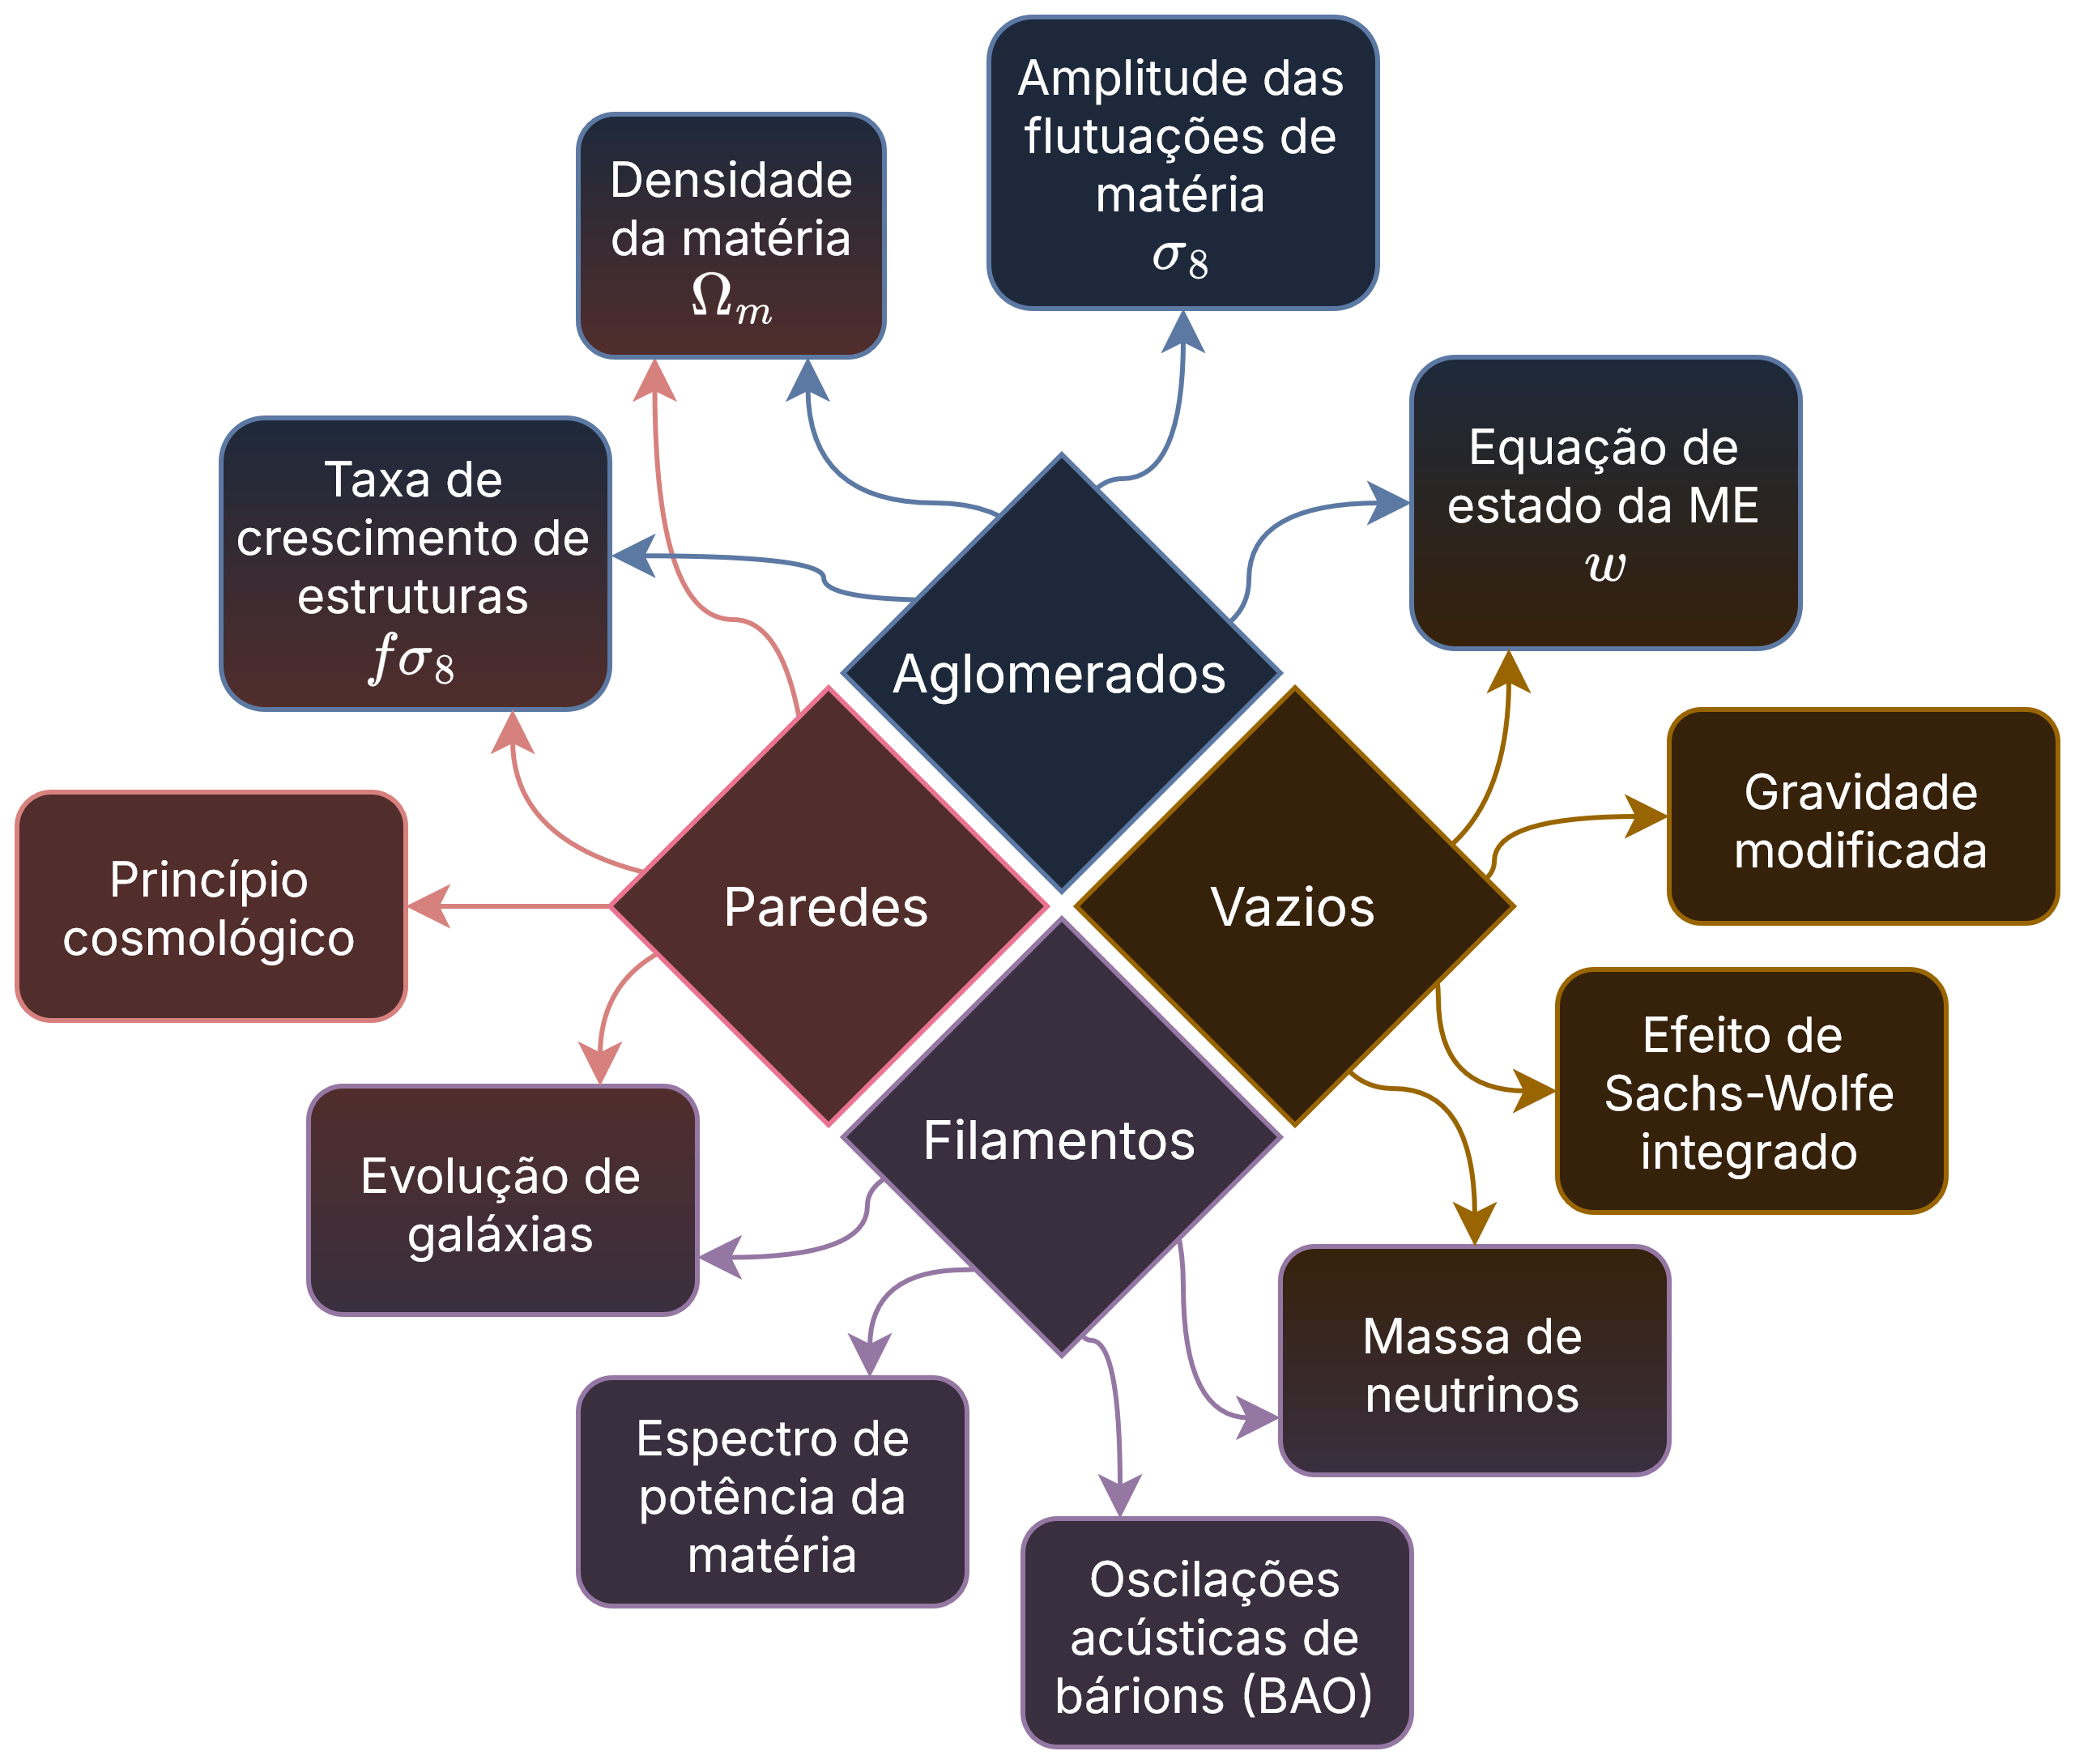
\includegraphics[height=7cm]{images/LSS.png}
%             \end{figure}
%         \end{column}
%         %
%         \begin{column}{0.36\textwidth}
%             \begin{splusbox}{}
%                 O problema é que estas estruturas são tridimensionais, mas nossas observações são projetadas (bidimensionais)
%             \end{splusbox}
%         \end{column}
%     \end{columns}
% \end{frame}


\begin{frame}[c]{Redshifts espectroscópicos e suas limitações}
    Uma forma de determinar a distância de objetos celestes vêm da lei de Hubble Lemaître (válida para objetos próximos):
    \vspace*{-0.5cm}
    \begin{figure}
        \centering
        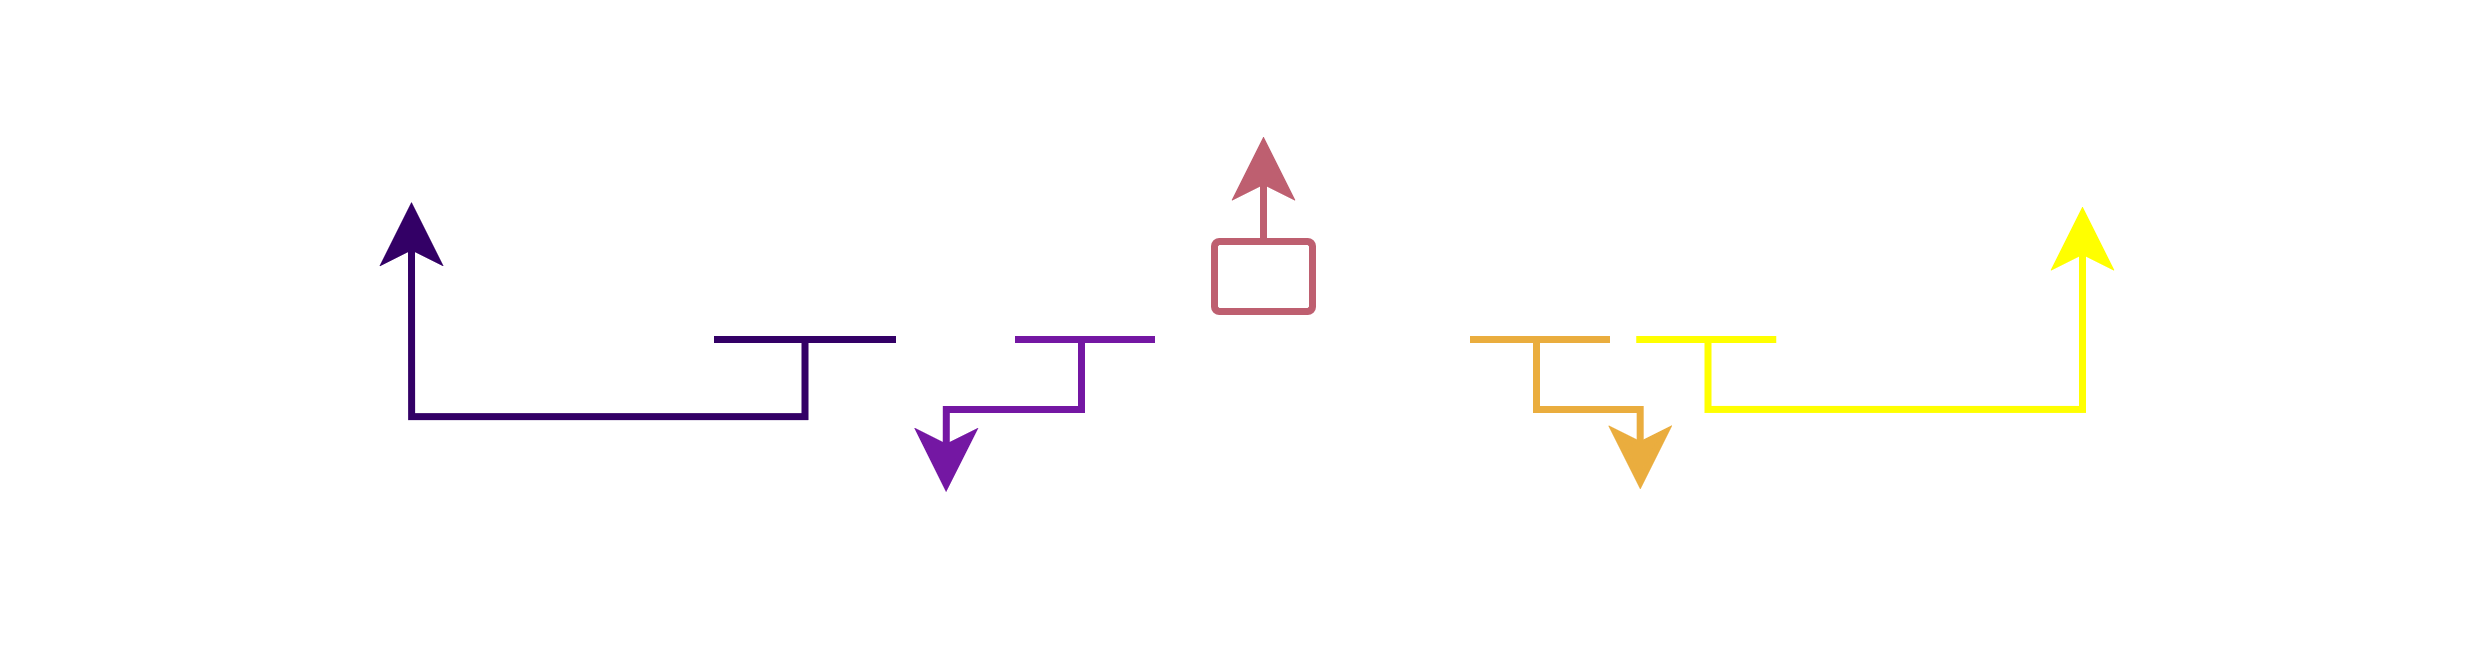
\includegraphics[width=0.8\linewidth]{script/images/hubble_law.png}
    \end{figure}
    \vspace*{-0.5cm}
    \begin{splusbox}{}
        \centering
        A observação de um espectro com alto sinal ruído demanda bastante tempo de observação, ainda mais para objetos fracos

        \vspace{0.3cm}
        É necessário encontrar uma alternativa
    \end{splusbox}
\end{frame}

\begin{frame}[c]{A alternativa: redshifts fotométricos}
    %\hspace*{1cm}
    \begin{columns}[c]
        \begin{column}{0.46\linewidth}
            \justifying
            Existem uma série de projetos que se baseiam em fotometria para produzir ciência.
            \begin{itemize}
                \justifying
                \item Pode ser considerada uma "aproximação" do espectro
                \item É obtida de forma muito mais rápida
                \item Pode alcançar magnitudes mais fracas
                \item É capaz de gerar dados para muitos objetos e grandes áreas
            \end{itemize}
        \end{column}
        \hspace*{-0.5cm}
        \begin{column}{0.46\linewidth}
            \begin{figure}
                \centering
                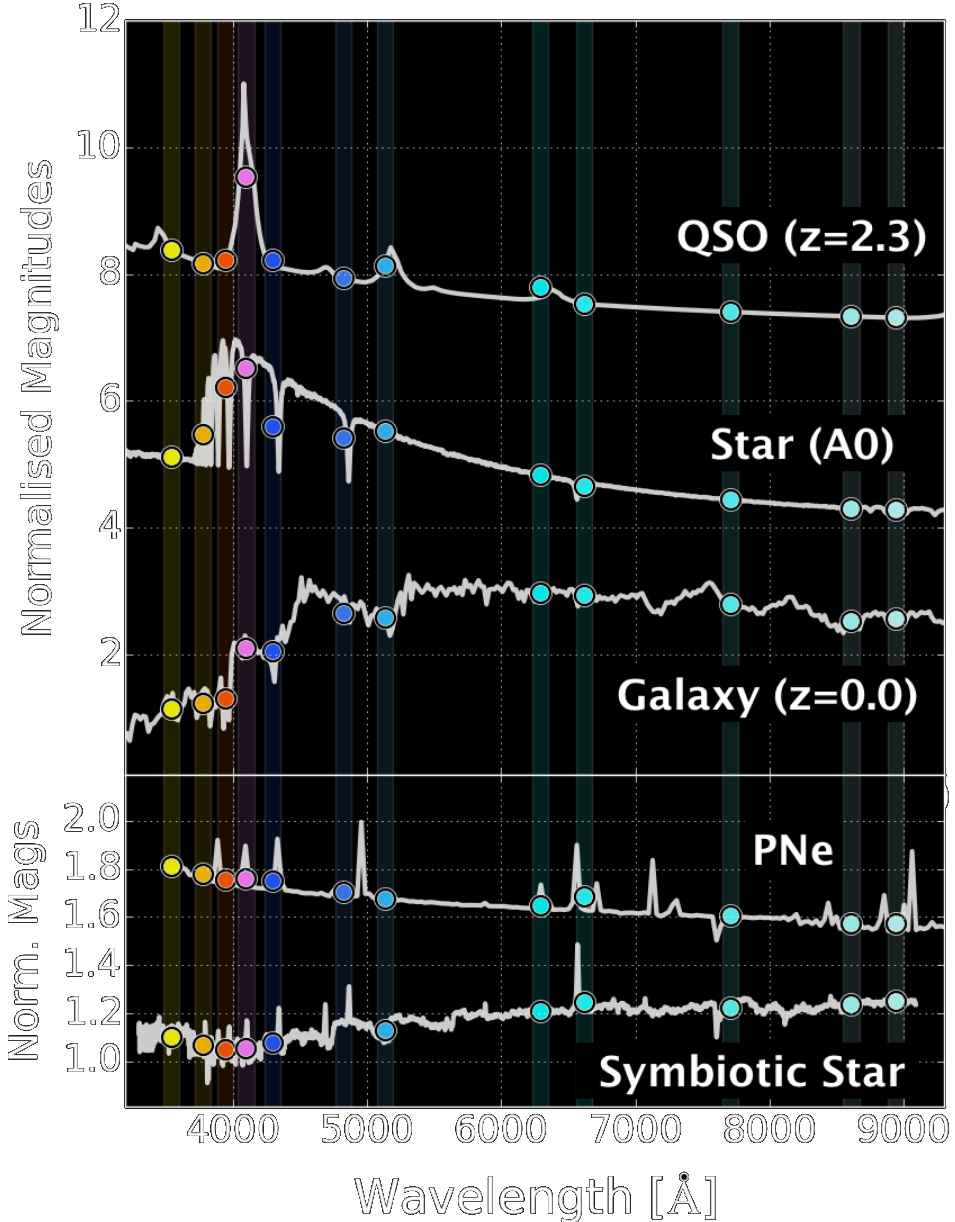
\includegraphics[height=5.5cm]{script/images/splus_spectra_sed.png}
                \caption{Mendes de Oliveira et al. (2019).}
            \end{figure}
        \end{column}
    \end{columns}
\end{frame}

\begin{frame}[c]{A alternativa: redshifts fotométricos}
    Redshifts fotométricos são estimados por três tipos de algoritmos: aprendizado de máquina, ajuste de templates e códigos híbridos.

    \begin{columns}[c]
        \footnotesize
        \begin{column}{0.46\textwidth}
            \begin{splusbox}{Aprendizado de máquina (ML)}
                \begin{itemize}
                    \justifying
                    \item[$\checkmark$] Se baseiam no uso de uma amostra de treinamento
                    \item[$\checkmark$] Flexível em relação a modelos (RFs, KNNs, SVMs)
                    \item[$\checkmark$] Podem ser mais precisos e rápidos que modelos de ajuste de template
                    \item[$\times$] Não fornecem uma classificação do objeto (exceto caso seja configurado para isso)
                    \item[$\times$] Sujeito à vieses devido aos dados
                \end{itemize}
            \end{splusbox}
        \end{column}

        \begin{column}{0.46\textwidth}
            \begin{splusbox}{Ajuste de templates (TF)}
                \begin{itemize}
                    \justifying
                    \item[$\checkmark$] Fazem uma comparação entre a fotometria de um objeto e uma biblioteca de templates
                    \item[$\checkmark$] Fornecem uma classificação do objeto junto ao $z_\text{phot}$
                    \item[$\checkmark$] Maior capacidade de extrapolação
                    \item[$\times$] Menos precisos, mais lentos
                    \item[$\times$] Sujeito à vieses devido à escolha dos templates
                \end{itemize}
            \end{splusbox}
        \end{column}

        % \begin{column}{0.33\linewidth}
        %     \begin{splusbox}{Híbridos}
        %         \footnotesize
        %         \begin{itemize}
        %             \item Combinam características de ML e TF
        %             \item Alguns códigos usam ML para gerar templates para um código de TF, outros usam templates para criar dados a serem usados num modelo de ML
        %         \end{itemize}
        %     \end{splusbox}
        % \end{column}
    \end{columns}
\end{frame}

\section{O objetivo}
\begin{frame}[c]{O objetivo}
    \begin{columns}[c]
        \begin{column}{0.46\linewidth}
            \begin{splusbox}{Redshifts fotométricos}
                \begin{itemize}
                    \justifying
                    \item Determinação de redshifts fotométricos de alta precisão
                    \item Funções de densidade de probabilidade bem calibradas
                    \item Galáxias até $z=0.8$ e magnitude 21 na banda \texttt{r}
                \end{itemize}
            \end{splusbox}
        \end{column}
        \begin{column}{0.46\linewidth}
            \begin{splusbox}{Estrutura em larga escala}
                \begin{itemize}
                    \justifying
                    \item Utilizar dados fotométricos para a reconstrução da LSS
                    \item Obter um mapeamento similar ao visto usando $z_\text{spec}$
                    %\item Possibilitar estudos que abrangem diferentes áreas da cosmologia
                \end{itemize}
                %Recuperação das estrutura da LSS, tal como vemos usando $z_\text{spec}$, a partir de estimativas fotométricas
            \end{splusbox}
        \end{column}
    \end{columns}

    \centering
    \begin{splusbox}{}
        Expandir o conjunto de dados que podemos usar para estudos em diferentes áreas da astronomia
    \end{splusbox}
\end{frame}

\section{Dados}
\begin{frame}[c]{Dados fotométricos}
    \begin{figure}
        \centering
        \begin{minipage}{0.48\textwidth}
            \centering
            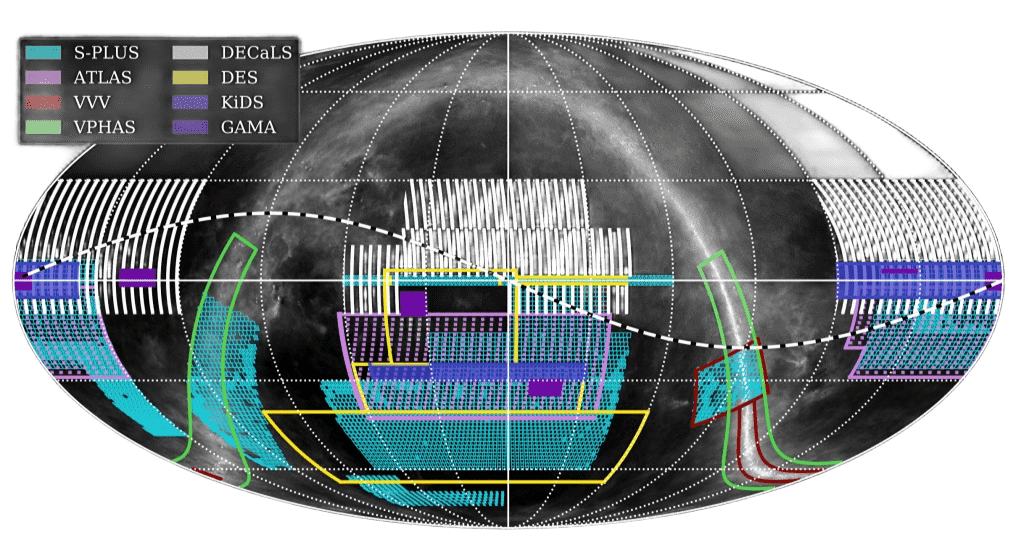
\includegraphics[width=\textwidth]{images/splus_survey_area.png}
            % \caption{}
        \end{minipage}
        \hfill
        \begin{minipage}{0.48\textwidth}
            \centering
            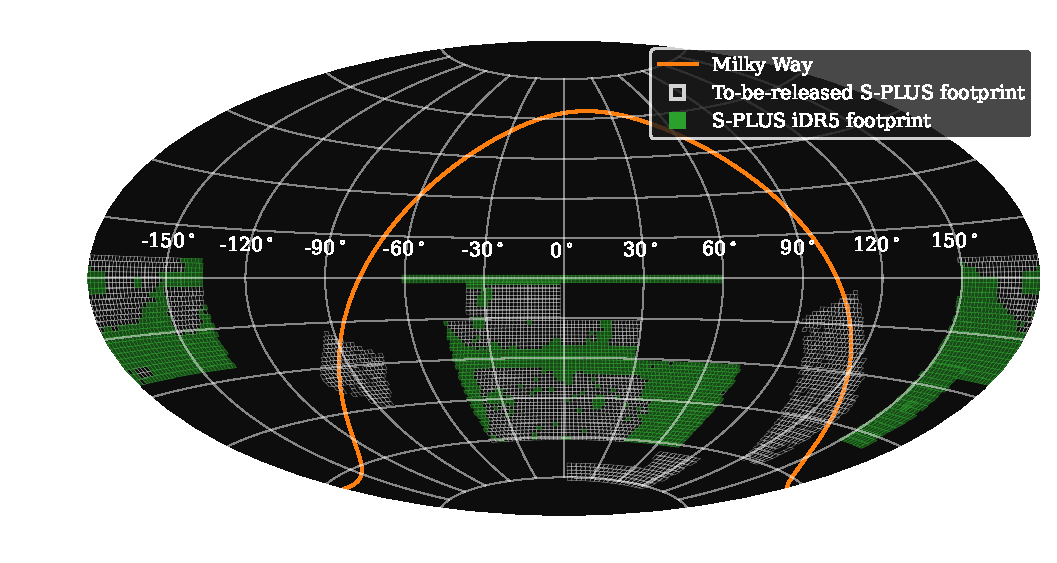
\includegraphics[width=\textwidth]{script/images/splus_footprint_idr5.pdf}
            % \caption{}
        \end{minipage}
    \end{figure}
\end{frame}

\begin{frame}[c]{Dados fotométricos}%[label=current]
    \textbf{DR4}: 3022,7 square degrees,\\
    \textbf{1629} Fields (each $\sim$2 square degrees)\\
    \textbf{Filters}
    \begin{figure}
        \centering
        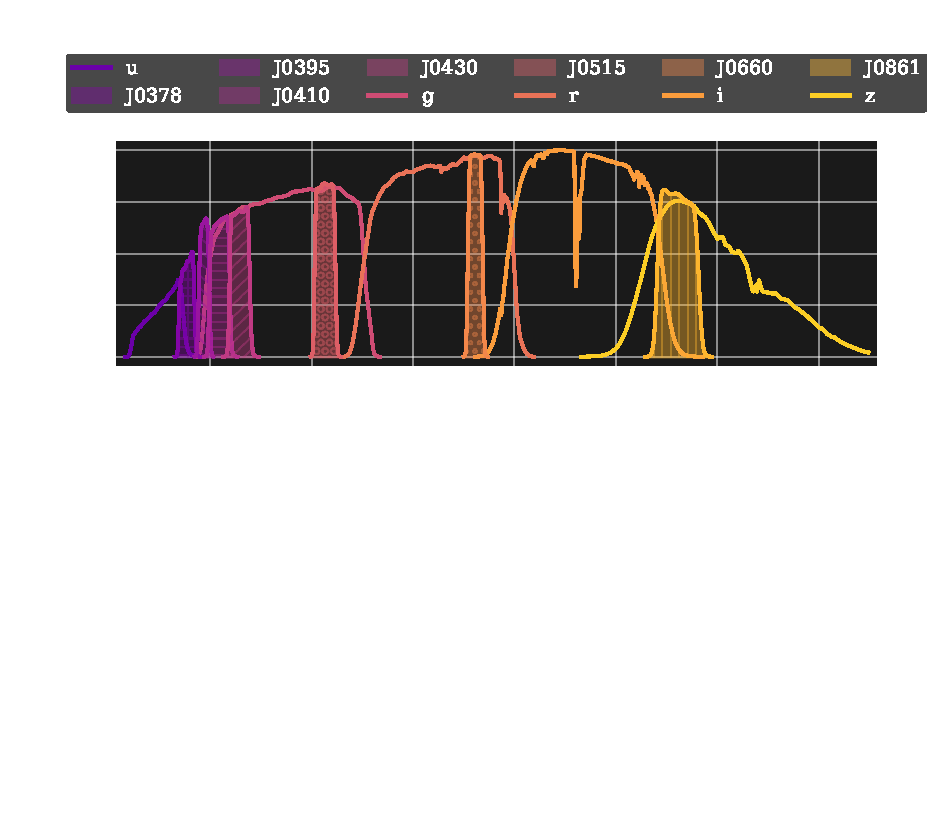
\includegraphics[width=\linewidth]{script/images/transmission_curves.pdf}
    \end{figure}
\end{frame}

\begin{frame}[c]{Dados fotométricos}
    \textbf{Fornax}\\
    \textbf{Run 1}: Faint objects detected near bright galaxies at Fornax distance\\
    \textbf{Run 2}: Better characterizes larger and brighter galaxies
    \begin{columns}[c]
        \begin{column}{0.48\linewidth}
                    \begin{figure}
                        \centering
                        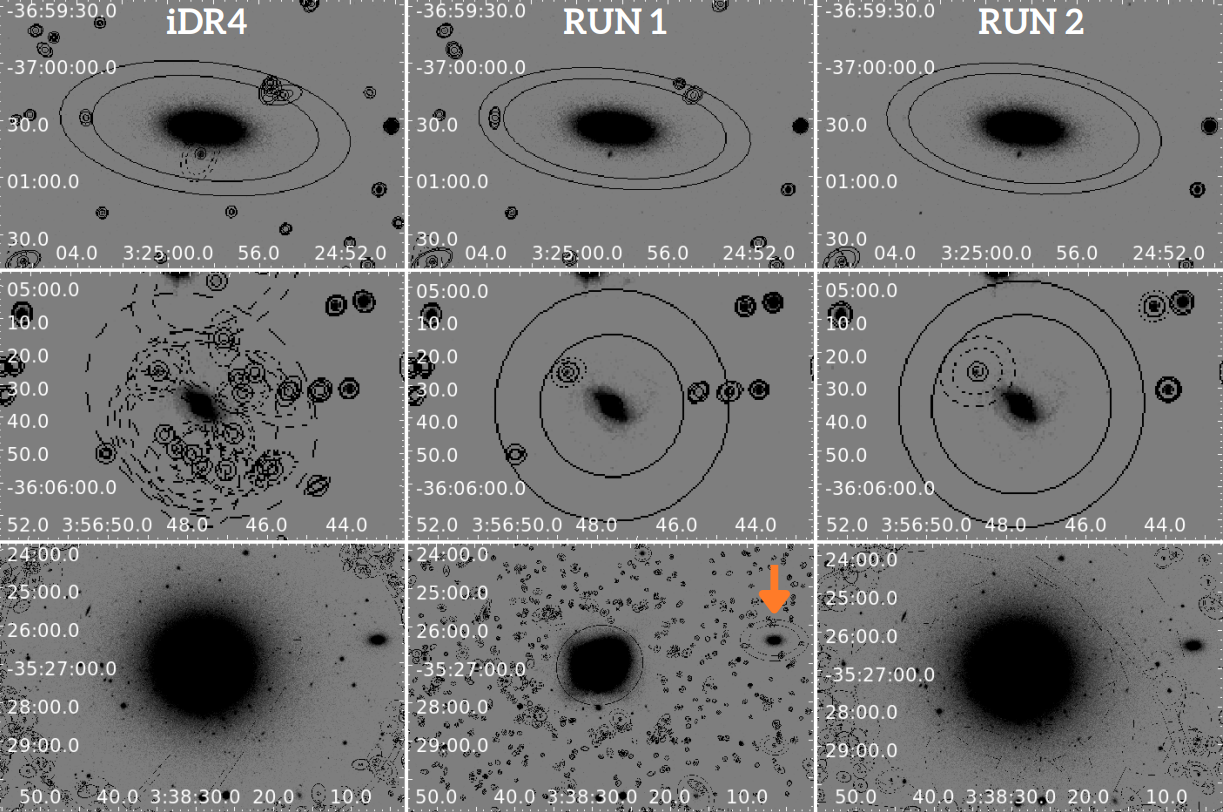
\includegraphics[width=\linewidth]{images/run1.png}
                        \caption{Haack,R.F.(2024)-https://arxiv.org/pdf/2404.10847}
                    \end{figure}
                \end{column}
        \begin{column}{0.48\linewidth}
                    \textbf{Extinction correction}
                    \begin{itemize}
                        \item Galaxy dust affects photometric measurements. Python dustmaps (Green, 2018)
                        \item Calculation of Extinction Coefficients. Python extinction (Barbary 2016)
                    \end{itemize}
                \end{column}
    \end{columns}
\end{frame}

\begin{frame}[c]{Cortes de qualidade na fotometria}
    \begin{splusbox}{Critérios de seleção}
        \begin{itemize}
            \item Magnitudes maiores que 30 foram descartadas (baixa qualidade e erros altos).
            \item Objetos com \texttt{flag0<3} também foram descartados.
            \item Banda \texttt{g\_APER\_6} como referência principal:
            \begin{itemize}
                \item Corte inferior: \texttt{g\_APER\_6} $>$ 13 (evitar saturação).
                \item Corte superior: \texttt{g\_APER\_6} $<$ 21 (minimizar contaminação por aglomerados globulares).
            \end{itemize}
        \end{itemize}
    \end{splusbox}

    \begin{splusbox}{Resultados}
        \begin{itemize}
            \item Total inicial: 2.9 milhões de objetos.
            \item Após cortes: 619.630 objetos restantes.
        \end{itemize}
    \end{splusbox}

\end{frame}

\begin{frame}[c]{Cortes de qualidade na fotometria}
    \begin{figure}
        \centering
            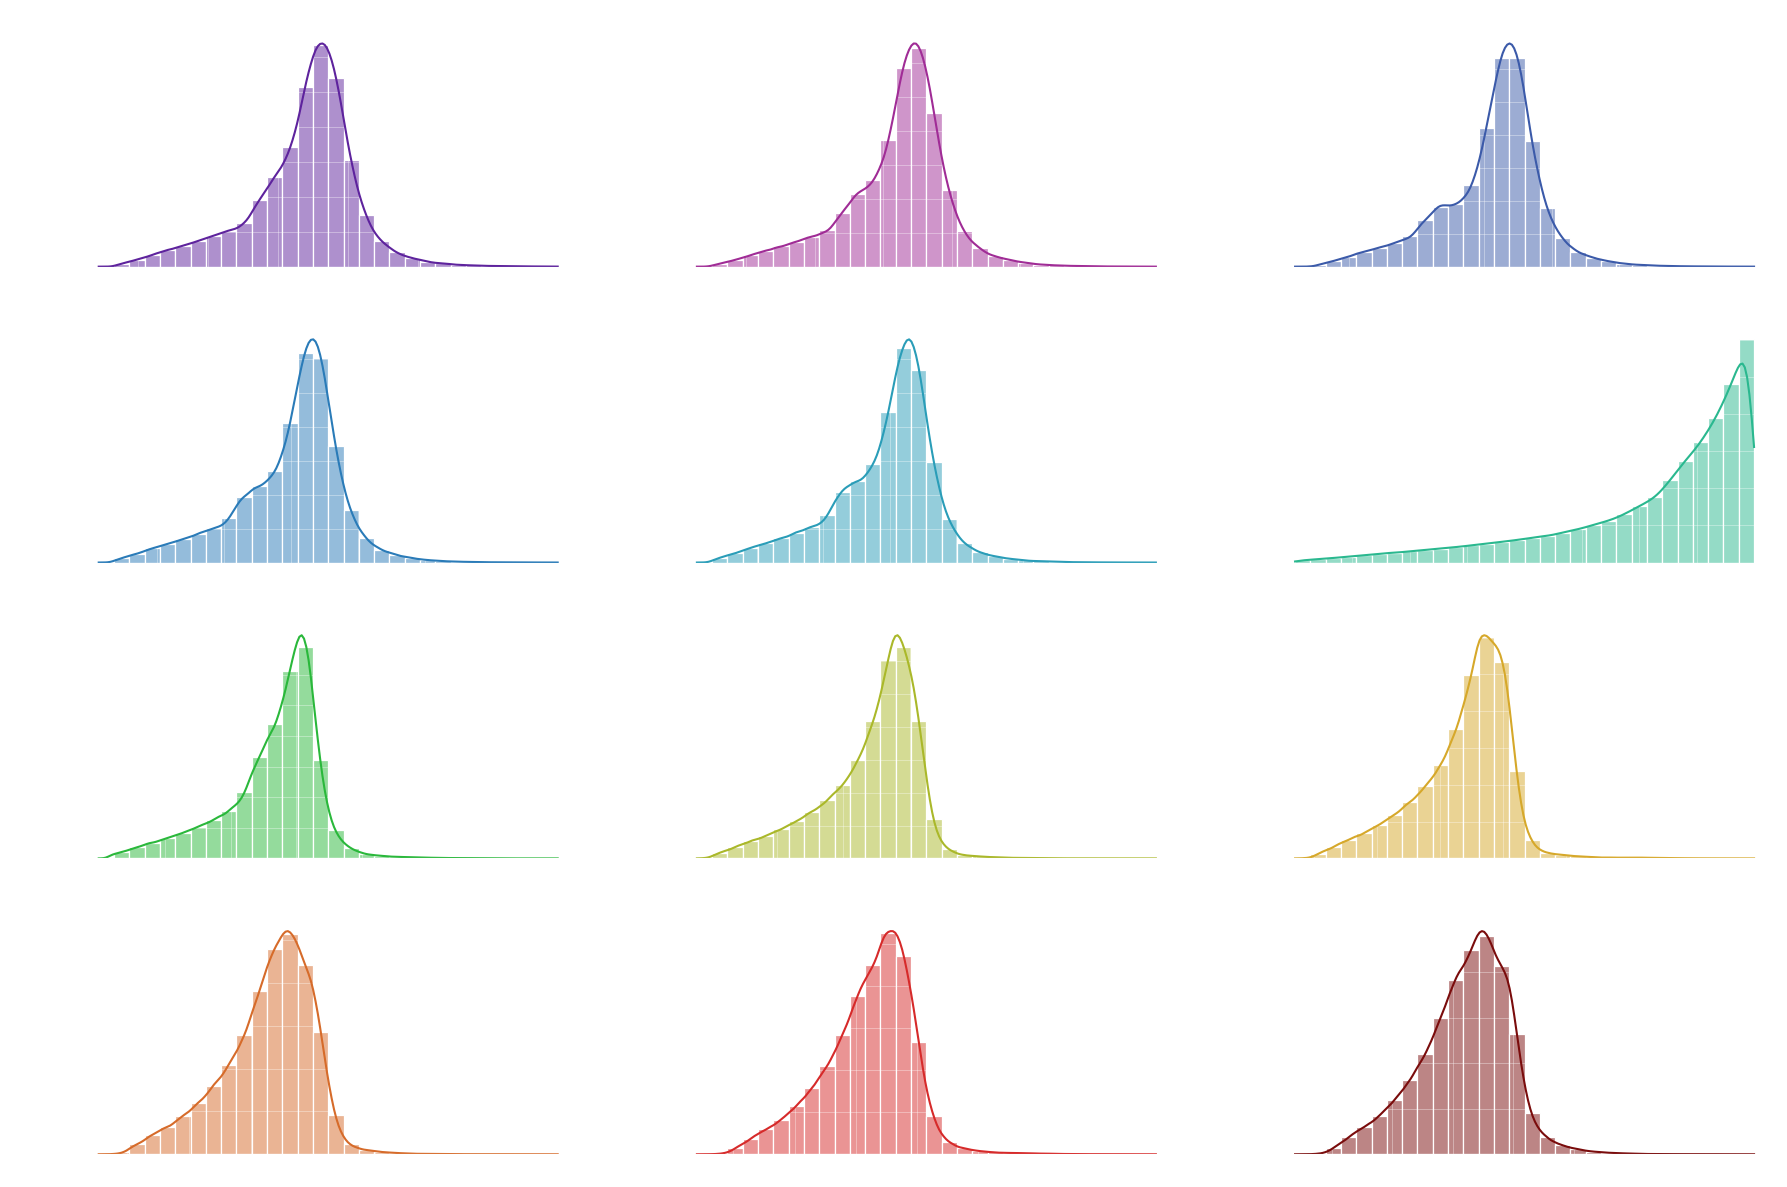
\includegraphics[width=\linewidth, height=6.5cm, keepaspectratio]{images/hist_distri_mags_data.png}
    \end{figure}
\end{frame}

\begin{frame}{Dados espectroscópicos {\small \textcolor{gray}{\url{(https://github.com/ErikVini/specz_compilation)}}}}
    \begin{columns}[c]
        \hspace{0.5cm}
        \begin{column}{0.40\textwidth}
            \begin{splusbox}{Informações do compilado}
                \begin{itemize}
                    \item Total de catálogos: 5097
                    \item Catálogos usados: 1872
                    \item Total de objetos: \mbox{8 437 460}
                    \item \underline{Pré era GPT!}
                \end{itemize}
            \end{splusbox}
        \end{column}
        %\hspace{-0.5cm}
        \begin{column}{0.50\textwidth}
            \begin{figure}
                \centering
                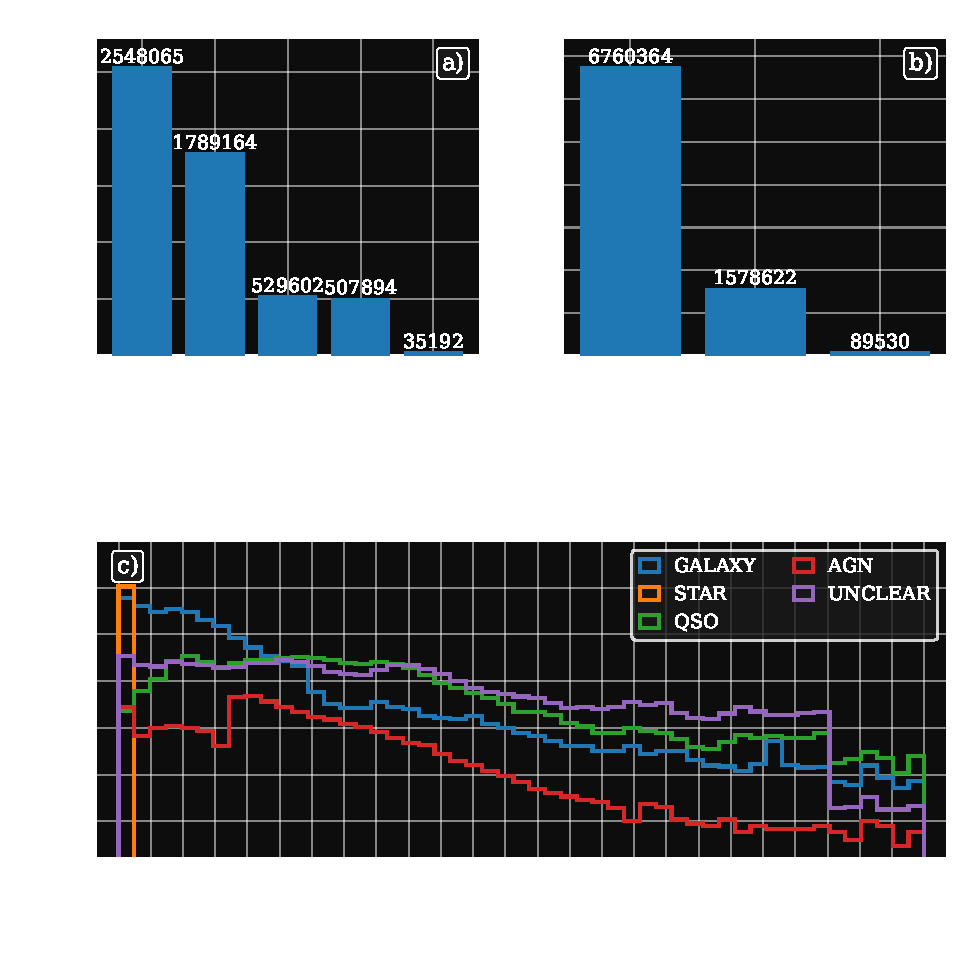
\includegraphics[height=7cm]{script/images/specz_distributions.pdf}
            \end{figure}
        \end{column}
    \end{columns}
\end{frame}

%%%%%%%%%%%%%%%%%%%%%%%%%%%%%%%%%%%%%%%%%%%%%%%%%%%%%%%%%%%%%%%%%%%%%%
\begin{frame}[c]{Distribuição das UCDs em Fornax}
    \begin{figure}
        \centering
        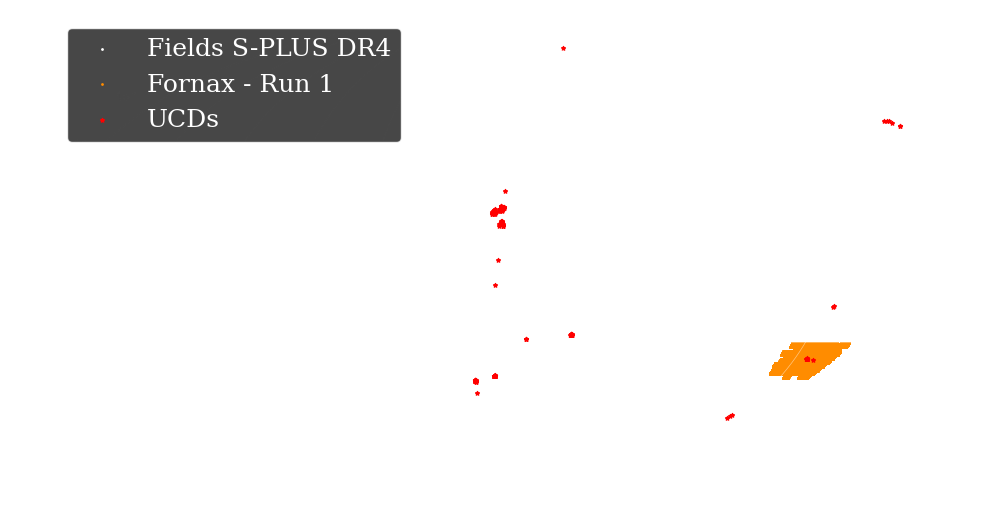
\includegraphics[width=0.8\linewidth, keepaspectratio]{images/ucds_sky.png}
    \end{figure}
\end{frame}

\begin{frame}[c]{Distribuição das UCDs em Fornax}
    \begin{figure}
        \centering
        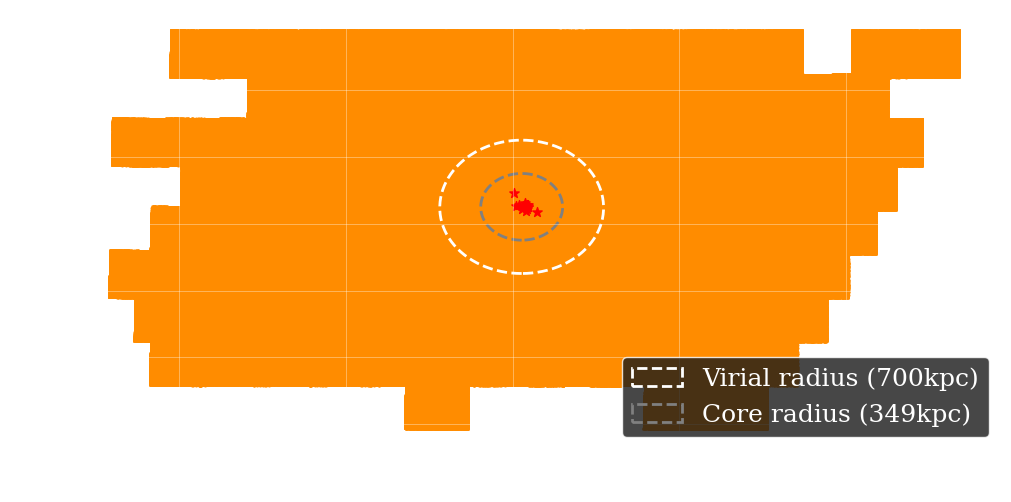
\includegraphics[width=0.8\linewidth, keepaspectratio]{images/zoom_fornax.png}
    \end{figure}
\end{frame}

\begin{frame}[c]{Distribuição das UCDs em Fornax}
    \begin{columns}[c]
        \begin{column}{0.48\textwidth}
            \centering
            \begin{table}[!ht]
                \centering
                \footnotesize
                \begin{tabular}{lc}
                    \toprule
                    \textbf{Parâmetro} & \textbf{Valor} \\ 
                    \midrule
                    Massa ($M_\odot$)$^1$ & $7 \pm 2 \times 10^{13}$ \\ 
                    Raio Virial ($Mpc$)$^1$ & 0.7 \\ 
                    Raio Virial ($graus$)$^1$ & 2 \\ 
                    Raio interno ($Mpc$)$^4$ & 0.349 \\ 
                    Raio interno ($graus$)$^4$ & 1 \\ 
                    $\sigma_v$ ($km \, s^{-1}$)$^3$ & 318 \\ 
                    Módulo de distância ($mag$)$^2$ & 31.51 \\ 
                    \bottomrule
                \end{tabular}
            \end{table}
        \end{column}
        \begin{column}{0.48\textwidth}
            \centering
            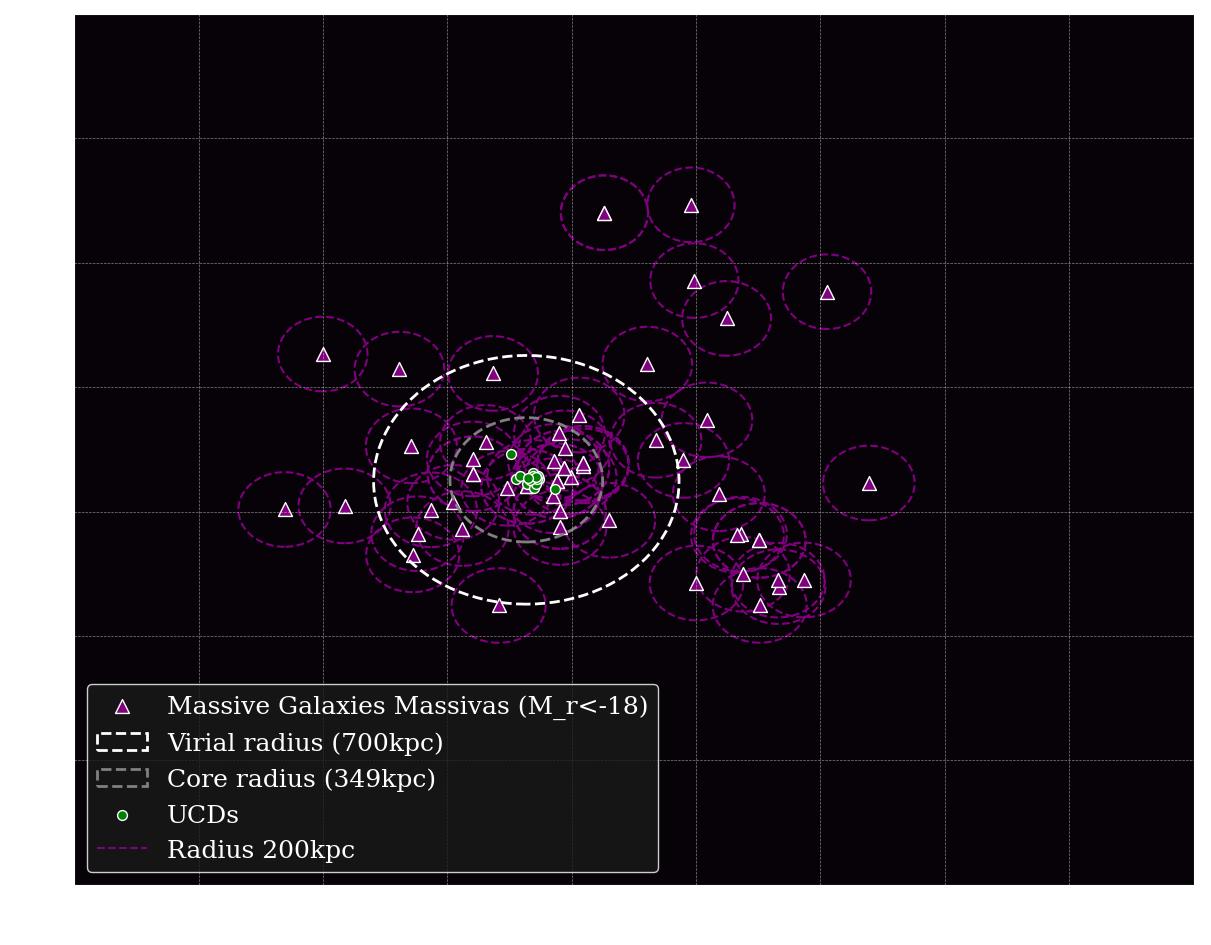
\includegraphics[width=\textwidth, height=0.48\textheight, keepaspectratio]{images/distribuicao_galaxias_massivas.png}
            \vspace{0.5cm}
            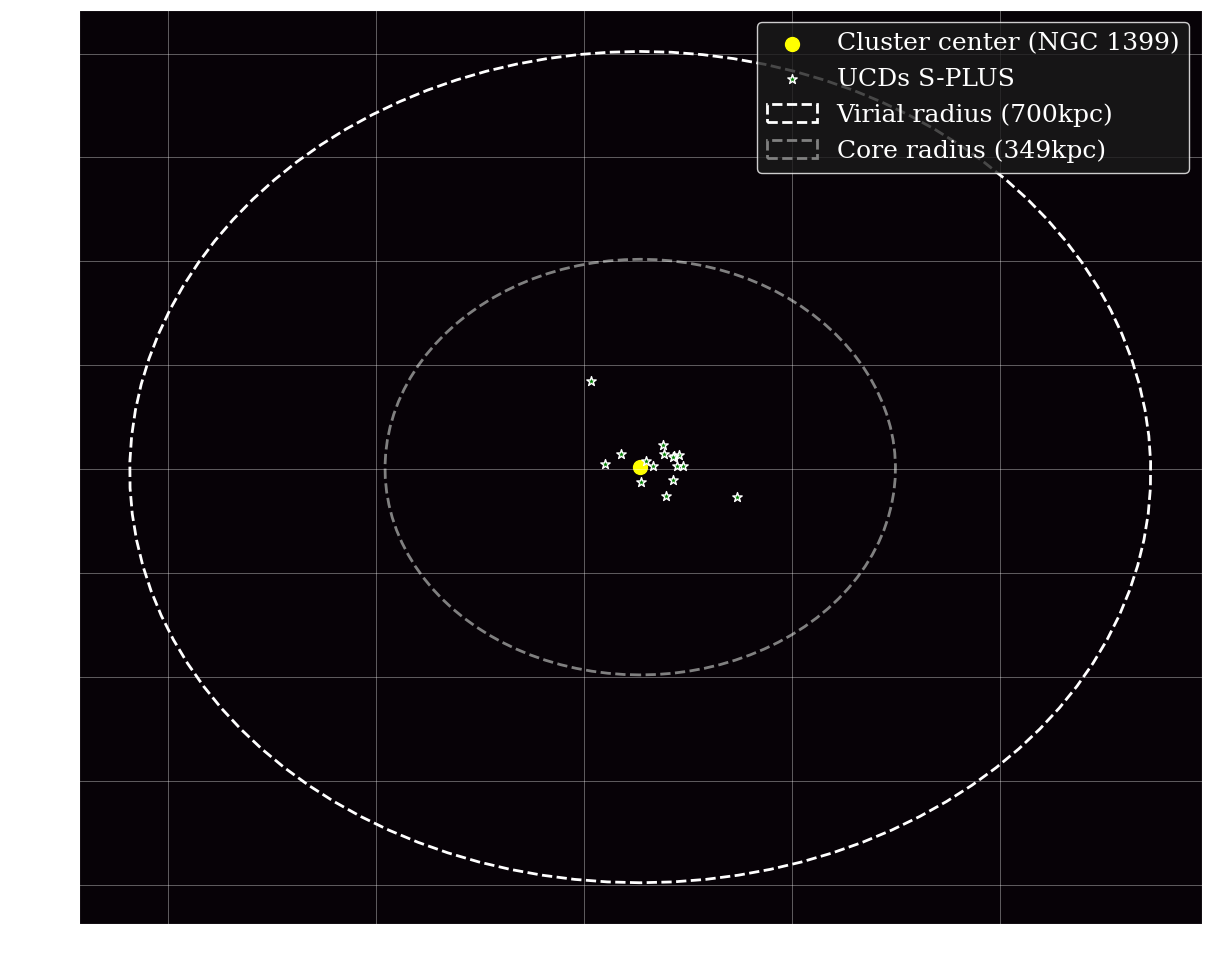
\includegraphics[width=\textwidth, height=0.48\textheight, keepaspectratio]{images/distribuicao_ucds_center.png}
        \end{column}
    \end{columns}
\end{frame}

\begin{frame}[c]{Propriedades das UCDs}
    \begin{table}[!ht]
        \centering
        \scriptsize
        \caption{Propriedades das UCDs de Mieske et al.(2008).}
        \begin{tabular}{lccccccc}
        \toprule
        Nome & Massa Total & $M/L_V$ & [Fe/H] & $r_h$ & $\sigma$ \\
        & ($10^6 \, M_\odot$) & & (dex) & (pc) & (km/s)\\
        \midrule
        UCD3, F-19 & $93.6 \pm 14.0$ & $4.69 \pm 0.70$ & -0.4 & 89.7 & 22.8 \\
        UCD1       & $32.1 \pm 3.9$  & $4.99 \pm 0.60$ & -0.7 & 22.4 & 27.1 \\
        F-24       & $24.5 \pm 7.8$  & $3.44 \pm 1.10$ & -0.4 & 29.5 & 21.4 \\
        UCD5       & $18.0 \pm 4.5$  & $3.37 \pm 0.85$ & -1.2 & 31.2 & 18.7 \\
        F-1a       & $16.2 \pm 3.8$  & $2.45 \pm 0.58$ & 0.0  & 23.1 & 18.7 \\
        F-9        & $14.1 \pm 3.6$  & $4.72 \pm 1.20$ & -0.8 & 9.1  & 25.7 \\
        F-5        & $13.7 \pm 2.4$  & $3.16 \pm 0.55$ & -0.3 & 5.0  & 34.5 \\
        F-6        & $12.5 \pm 2.4$  & $5.32 \pm 1.00$ & 0.2  & 7.3  & 27.3 \\
        F-7        & $10.5 \pm 1.4$  & $4.21 \pm 0.57$ & -1.3 & 14.9 & 20.1 \\
        F-12       & $8.3 \pm 2.9$   & $2.36 \pm 0.83$ & -0.4 & 10.3 & 22.9 \\
        F-11       & $5.7 \pm 3.7$   & $1.64 \pm 1.10$ & -0.9 & 3.6  & 26.2 \\
        F-34       & $5.5 \pm 1.3$   & $3.17 \pm 0.74$ & -0.9 & 4.0  & 24.6 \\
        F-22       & $5.3 \pm 1.0$   & $2.13 \pm 0.39$ & -0.4 & 10.0 & 22.8 \\
        F-53       & $3.9 \pm 1.0$   & $2.66 \pm 0.69$ & -0.9 & 4.4  & 19.6 \\
        F-51       & $3.5 \pm 0.9$   & $2.38 \pm 0.62$ & -0.8 & 4.2  & 20.1 \\
        F-59       & $1.3 \pm 0.6$   & $0.94 \pm 0.43$ & -2.1 & 5.7  & 9.8  \\
        \bottomrule
        \end{tabular}
        \label{ucds_fornax_propriedades}
    \end{table}
\end{frame}

\begin{frame}[c]{Propriedades das UCDs}
    \begin{columns}[c]
        \begin{column}{0.48\textwidth}
            \begin{table}[!ht]
                \centering
                \scriptsize
                \begin{tabular}{lccc}
                    \toprule
                    Nome & spec-$z$ & $g$ & zml \\
                    \midrule
                    UCD3 & 0.0053 & 18.47 & 0.03 \\
                    UCD1 & 0.0052 & 19.75 & 0.08 \\
                    F-24 & 0.0063 & 19.66 & 0.04 \\
                    UCD5 & 0.0045 & 19.71 & 0.04 \\
                    F-1a & 0.0042 & 19.66 & -    \\
                    F-9  & 0.0058 & 20.85 & 0.07 \\
                    F-5  & 0.0057 & 20.54 & -    \\
                    F-6  & 0.0037 & 20.48 & -    \\
                    F-7  & 0.0050 & 20.89 & 0.16 \\
                    F-12 & 0.0055 & 20.37 & -    \\
                    F-11 & 0.0059 & 20.40 & -    \\
                    F-34 & 0.0054 & 20.79 & -    \\
                    F-22 & 0.0034 & 20.69 & 0.06 \\
                    F-53 & 0.0020 & 21.57 & -    \\
                    F-51 & 0.0041 & 22.23 & -    \\
                    F-59 & 0.0061 & 21.47 & -    \\
                    \bottomrule
                \end{tabular}
                \label{tab:ucds_know_z_gmag}
            \end{table}
        \end{column}
        \begin{column}{0.48\textwidth}
            \centering
            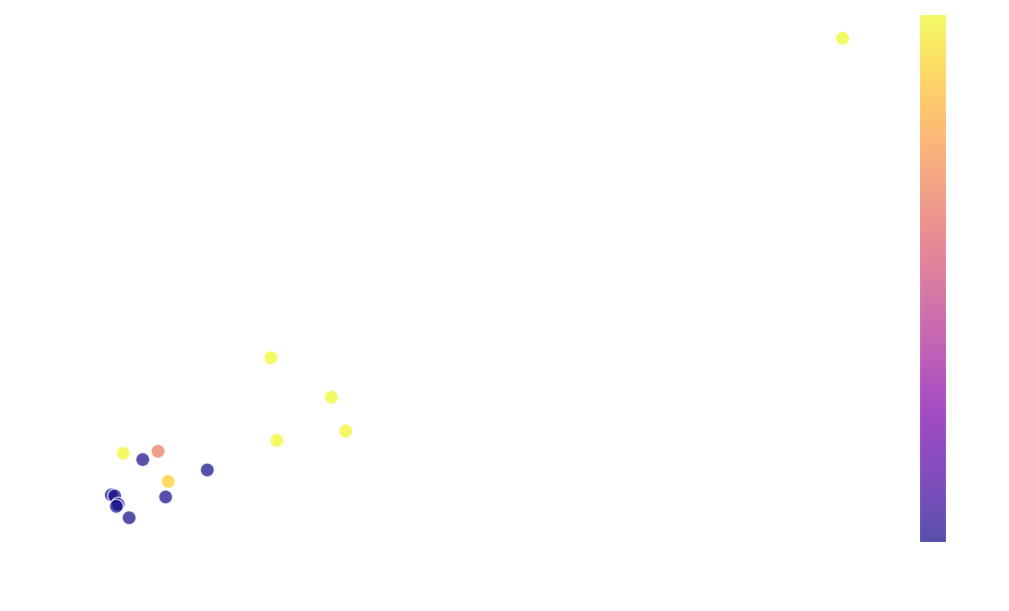
\includegraphics[width=\textwidth, height=0.48\textheight]{images/r_h_M_ucds.png}
            \vspace{0.5cm}
            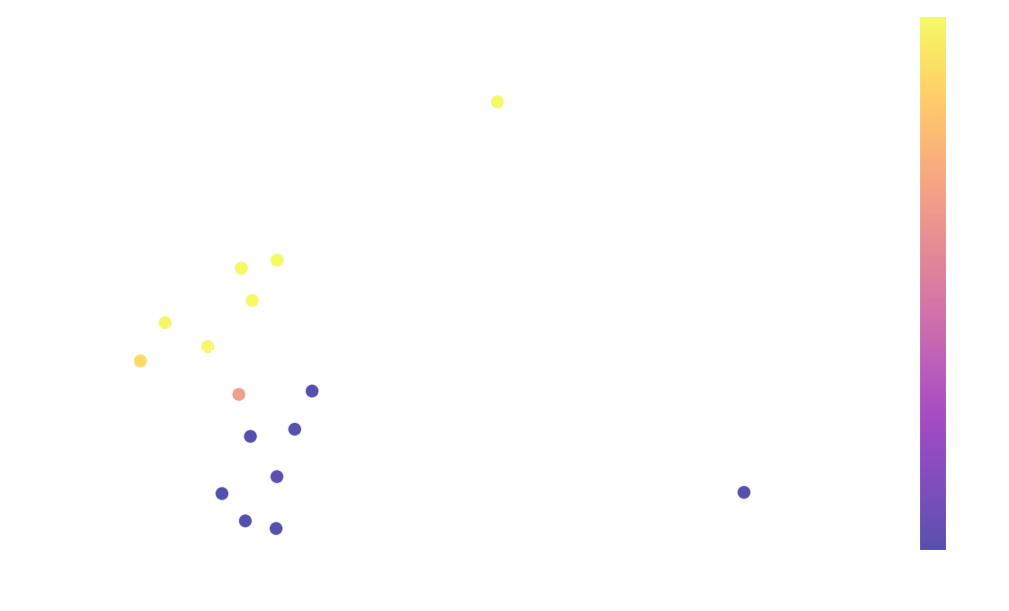
\includegraphics[width=\textwidth, height=0.48\textheight]{images/distribuicao_fwhm_image_r_r_aper6_ucds_fornax.png}
        \end{column}
    \end{columns}
\end{frame}

\section{Aprendizado de máquina}
\begin{frame}[c]{Procura de UCDs com Aprendizado de Máquina}
    \begin{splusbox}{Objetivo}
        \begin{itemize}
            \item Identificar candidatas a galáxias ultra-compactas no aglomerado de Fornax.
            \item Classificar objetos em duas categorias principais:
            \begin{itemize}
                \item Compactos.
                \item Extensos.
            \end{itemize}
            \item Separar objetos com base em suas características morfológicas e fotométricas.
        \end{itemize}
    \end{splusbox}
    \textbf{Identificar dentro do grupo de objetos compactos, aqueles que possuem características fotométricas semelhantes às de galáxias extensas.}
\end{frame}

\begin{frame}[c]{Amostra de Treino e Valores Faltantes}
    \begin{columns}[c]
        \begin{column}{0.48\textwidth}
            \begin{splusbox}{Amostra de Treino}
                \begin{itemize}
                    \item Divisão em classes:
                    \begin{itemize}
                        \item Classe 0: Compactos.
                        \item Classe 1: Extensos.
                    \end{itemize}
                    \item Total de objetos: 545.267.
                    \item Treinamento: 80\% dos dados.
                    \item Teste: 20\% dos dados.
                \end{itemize}
            \end{splusbox}
        \end{column}
        \begin{column}{0.48\textwidth}
            \begin{splusbox}{Valores Faltantes}
                \begin{itemize}
                    \item Imputação com MICE (Método de Imputação Múltipla).
                    \item 27\% dos objetos possuem pelo menos 1 valor faltante.
                    \item Dados faltantes tratados para garantir consistência.
                \end{itemize}
            \end{splusbox}
        \end{column}
    \end{columns}
\end{frame}

\begin{frame}[c]{Distribuição de Valores Faltantes}
    \vspace{0.5cm}
    \begin{figure}
        \centering
        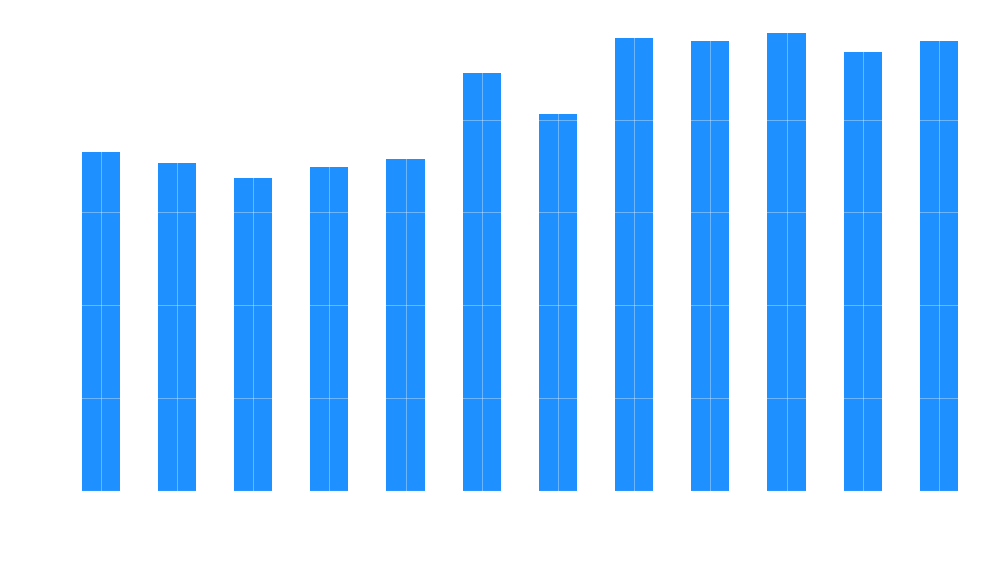
\includegraphics[width=0.8\linewidth, height=6cm, keepaspectratio]{images/missing_values_hist.png}
        \caption{Distribuição de valores faltantes.}
    \end{figure}
\end{frame}

\begin{frame}[c]{Amostra de treino}
    \begin{columns}[c]
        \begin{column}{0.48\textwidth}
            \vspace{0.5cm} % Adiciona espaço acima dos gráficos
            \hspace{0.5cm} % Adiciona espaço horizontal para afastar os gráficos do título
            \begin{figure}
                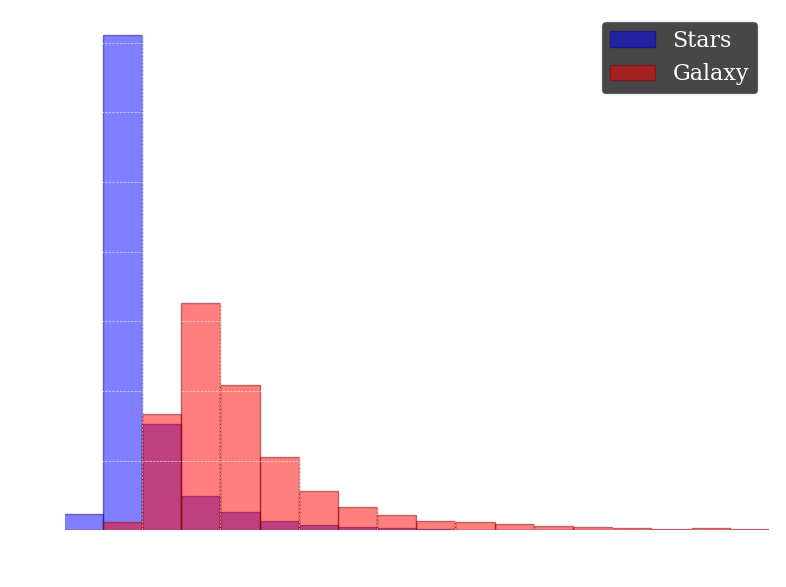
\includegraphics[width=\linewidth, height=0.44\textheight, keepaspectratio]{images/distribution_of_stars_and_galaxies.png}
                \vspace{0.5cm}
                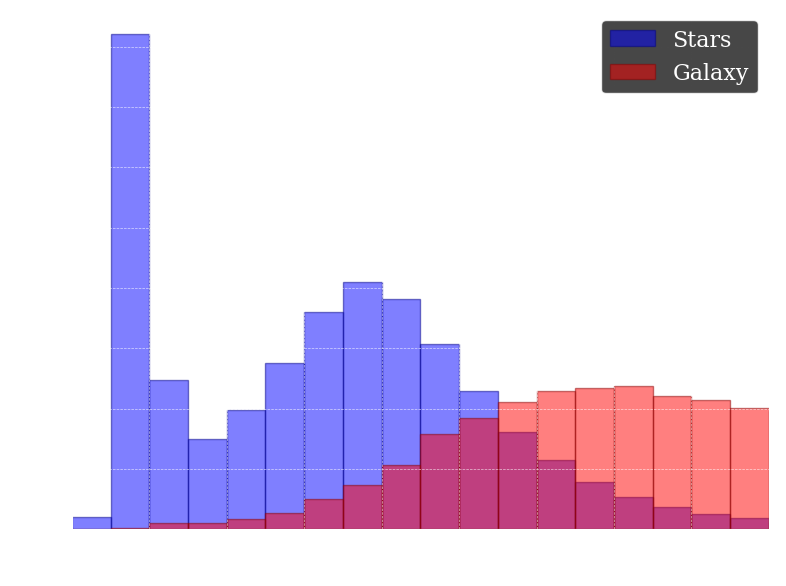
\includegraphics[width=\linewidth, height=0.44\textheight, keepaspectratio]{images/distribution_of_stars_and_galaxies_u.png}
            \end{figure}
        \end{column}
        \begin{column}{0.48\textwidth}
            \footnotesize
            \begin{itemize}
                \item \textbf{Precisão:} $\frac{\text{TP}}{\text{TP} + \text{FP}}$
                \item \textbf{Completeness:} $\frac{\text{TP}}{\text{TP} + \text{FN}}$
                \item \textbf{F1-Score:} $2 \cdot \frac{\text{Precisão} \cdot \text{Completeness}}{\text{Precisão} + \text{Completeness}}$
            \end{itemize}
            \begin{figure}
                \centering
                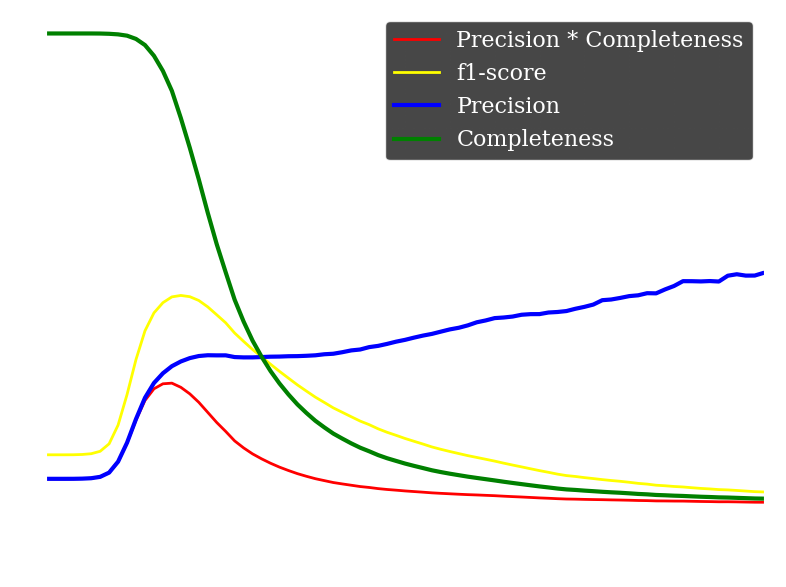
\includegraphics[width=\linewidth, height=0.5\textheight, keepaspectratio]{images/purity_completeness.png}
            \end{figure}
        \end{column}
    \end{columns}
\end{frame}

\begin{frame}[c]{Amostra de treino}
    \begin{columns}[c]
        \begin{column}{0.3\textwidth}
            \begin{splusbox}{\scriptsize Critérios de Classificação}
                \scriptsize
                \begin{itemize}
                    \item Compactos: FWHM $<$ 2 pixels.
                    \item Extensos: FWHM $>$ 2.5 pixels.
                    \item Dados entre 2 e 2.5 pixels não usados no treinamento.
                \end{itemize}
            \end{splusbox}
        \end{column}
        \begin{column}{0.7\textwidth}
            \centering
            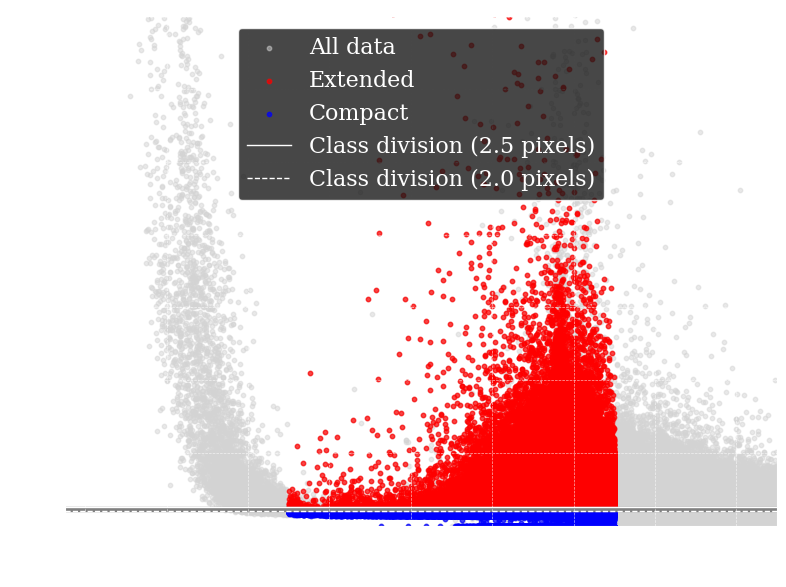
\includegraphics[width=\linewidth]{images/amostra_treino.png}
        \end{column}
    \end{columns}
\end{frame}

\begin{frame}[c]{Amostra de Treino}
    \begin{columns}[c]
        \begin{column}{0.48\textwidth}
            \begin{splusbox}{Divisão da Amostra}
                \begin{itemize}
                    \item Total de objetos: 545.267.
                    \item Treinamento: 80\% (436.213 objetos).
                    \item Teste: 20\% (109.054 objetos).
                    \item Classe 0 (compactos): 242.085 no treino, 60.522 no teste.
                    \item Classe 1 (extensos): 194.128 no treino, 48.532 no teste.
                \end{itemize}
            \end{splusbox}
        \end{column}
        \begin{column}{0.48\textwidth}
            \begin{splusbox}{Parâmetros Utilizados}
                \begin{itemize}
                    \item 12 magnitudes corrigidas pela extinção (\texttt{APER\_6}).
                    \item 66 combinações possíveis de cores.
                    \item Dados entre 2 e 2.5 pixels (FWHM) não usados no treinamento.
                \end{itemize}
            \end{splusbox}
        \end{column}
    \end{columns}
\end{frame}

\begin{frame}[c]{Classificador KNN}
    K-Nearest Neighbors (KNN) 
    \begin{columns}[c]
        \begin{column}{0.48\linewidth}
            \vspace{-1.5cm} % Ajusta o espaço vertical para começar mais acima
            \begin{itemize}
                \item Algoritmo supervisionado que classifica objetos com base nos vizinhos mais próximos.
                \item Simples e eficiente para conjuntos de dados menores.
                \item Utiliza a distância entre objetos no espaço de parâmetros para classificação.
            \end{itemize}
        \end{column}
        \begin{column}{0.48\linewidth}
            \vspace{-1cm} % Ajusta o espaço vertical para começar mais acima
            \begin{figure}
                \centering
                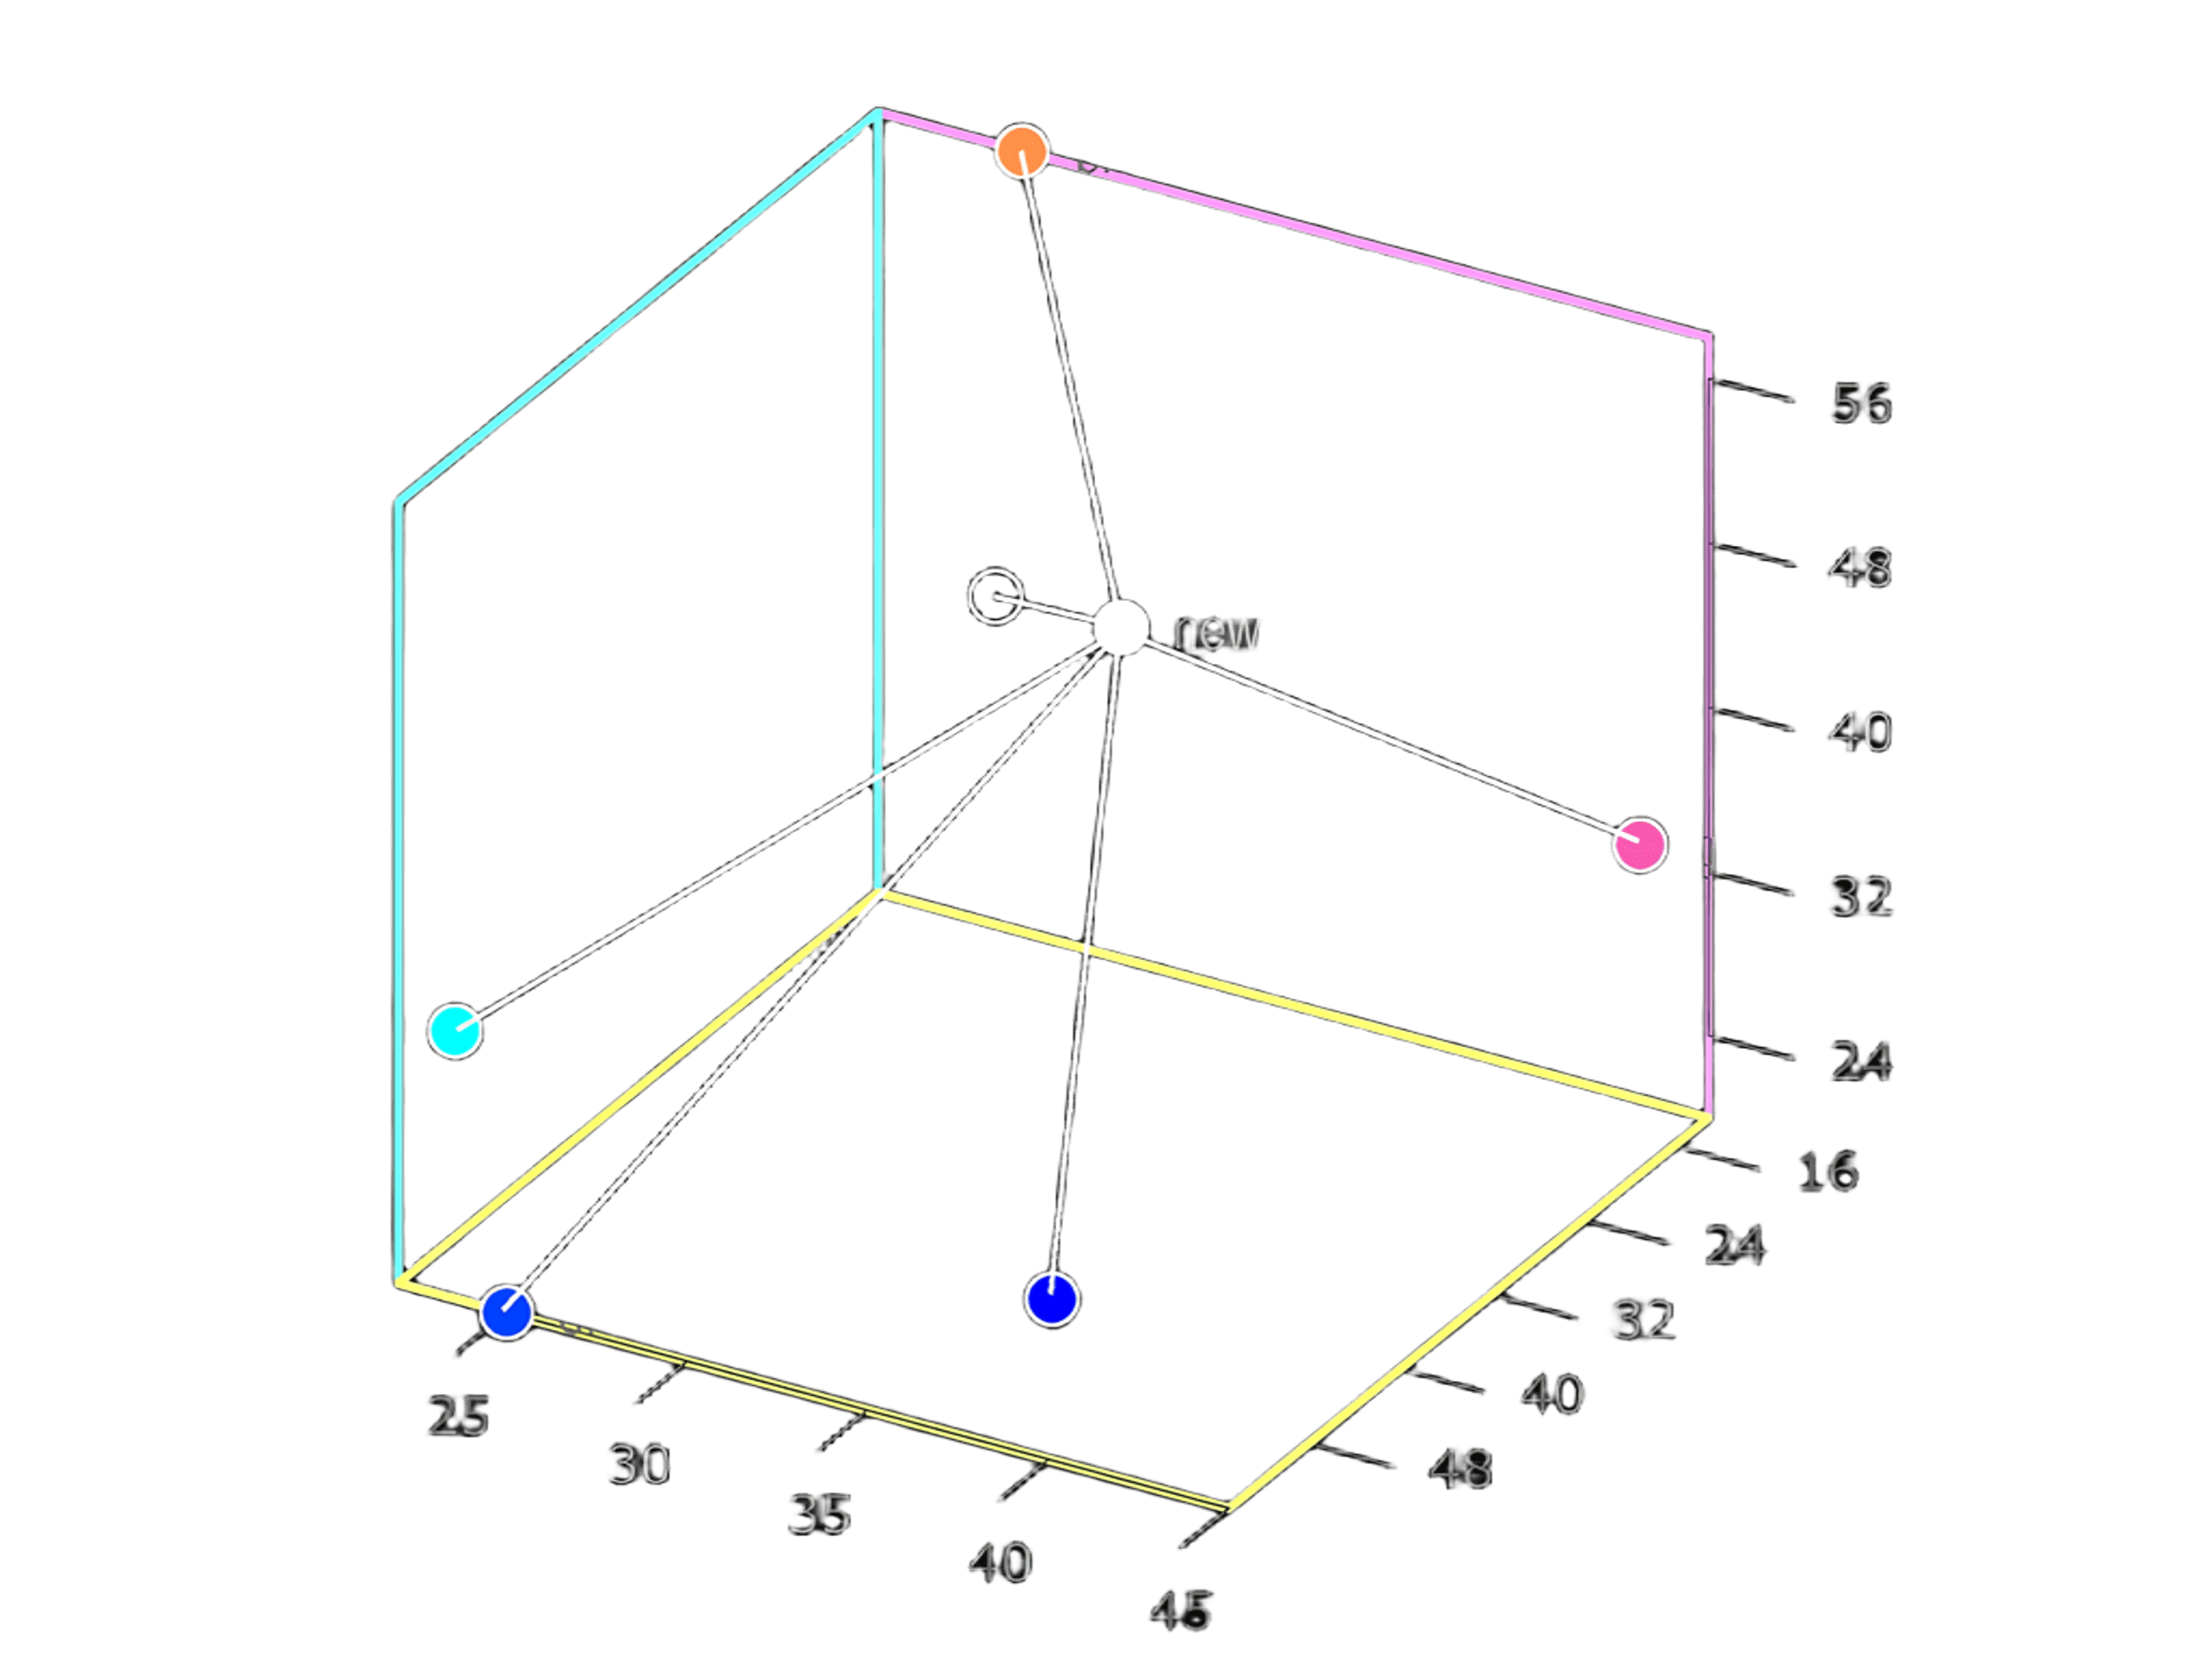
\includegraphics[height=4cm]{images/knn_example1.png}
                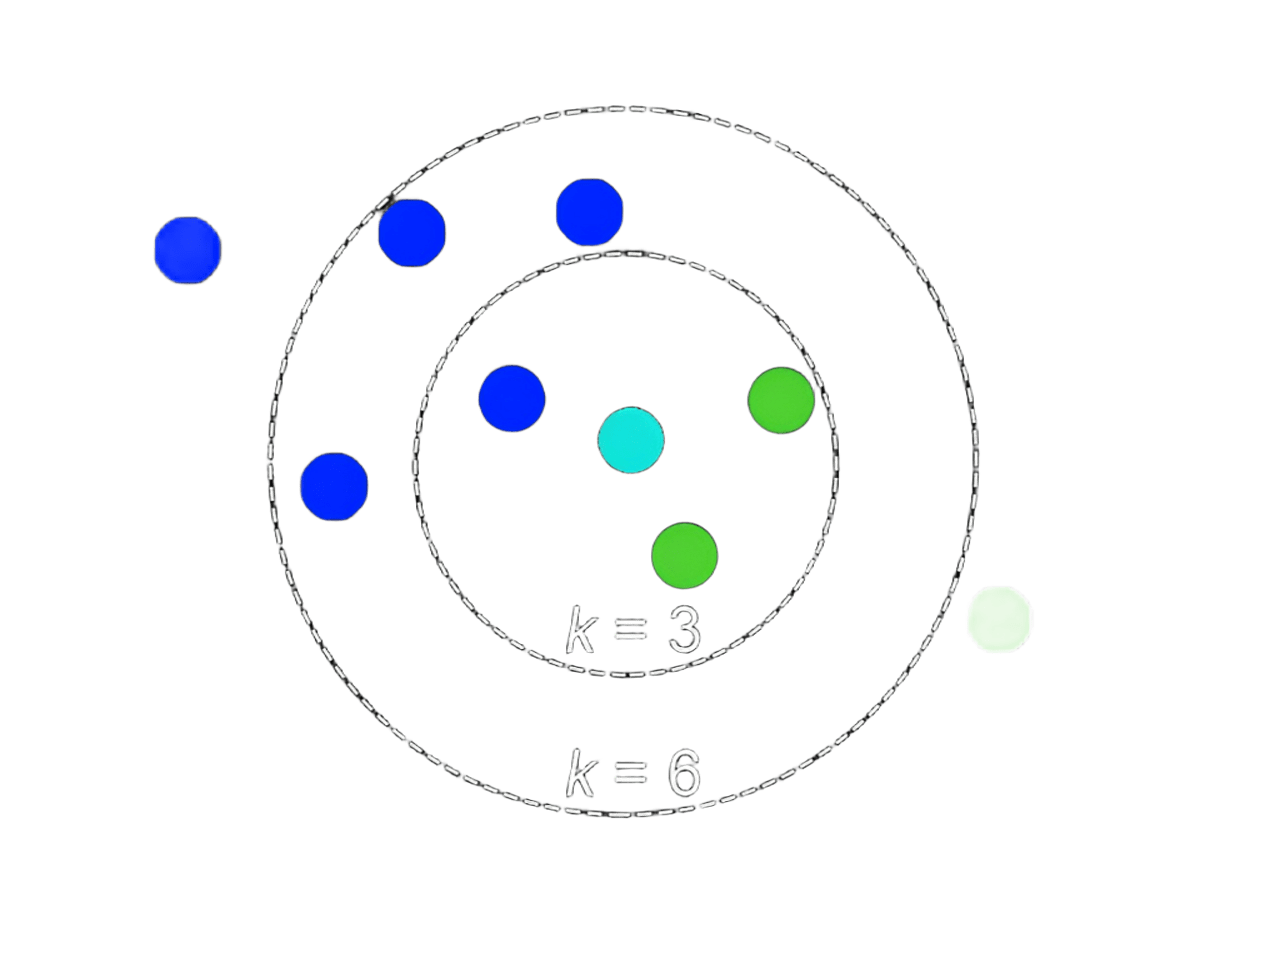
\includegraphics[height=4cm]{images/knn_example2.png}
            \end{figure}
        \end{column}
    \end{columns}
\end{frame}

\begin{frame}[c]{Classificador RF}
    Random Forest (RF)
    \begin{columns}[c]
        \begin{column}{0.48\linewidth}
            \vspace{-1.5cm} % Ajusta o espaço vertical para começar mais acima
            \begin{itemize}
                \item Algoritmo supervisionado baseado em múltiplas árvores de decisão.
                \item Combina os resultados de várias árvores para melhorar a precisão.
                \item Robusto contra overfitting em muitos casos.
                \item Eficiente para conjuntos de dados grandes e com muitas features.
            \end{itemize}
        \end{column}
        \begin{column}{0.48\linewidth}
            \vspace{-1cm} % Ajusta o espaço vertical para começar mais acima
            \begin{figure}
                \centering
                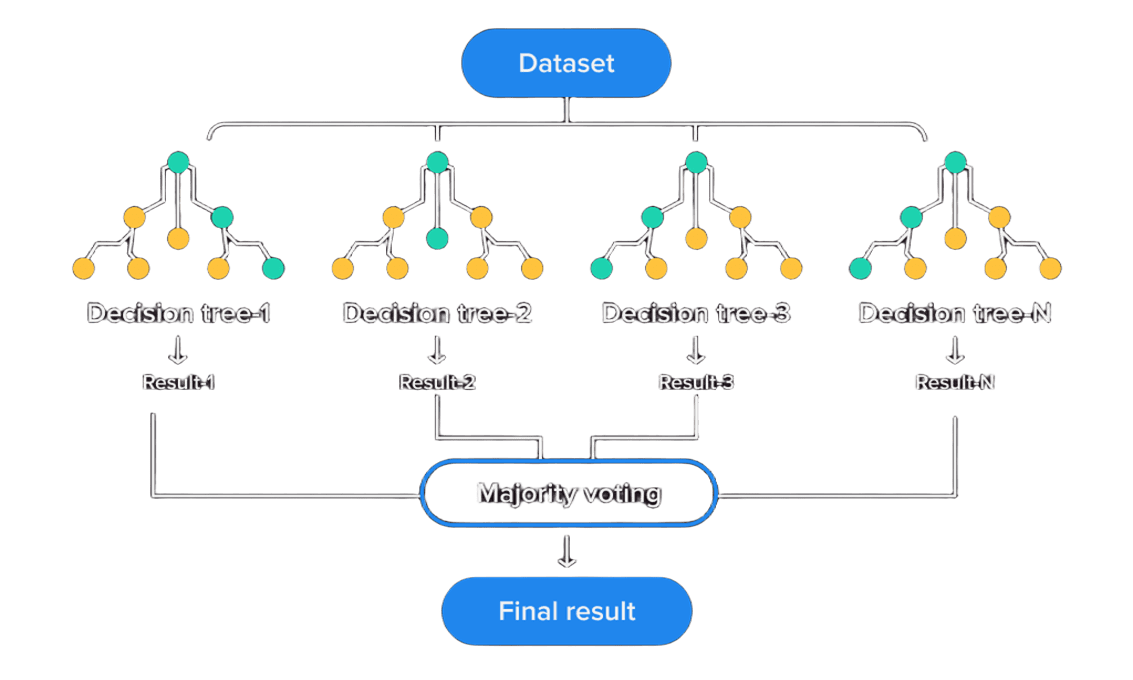
\includegraphics[height=4cm]{images/rf_example1.png}
                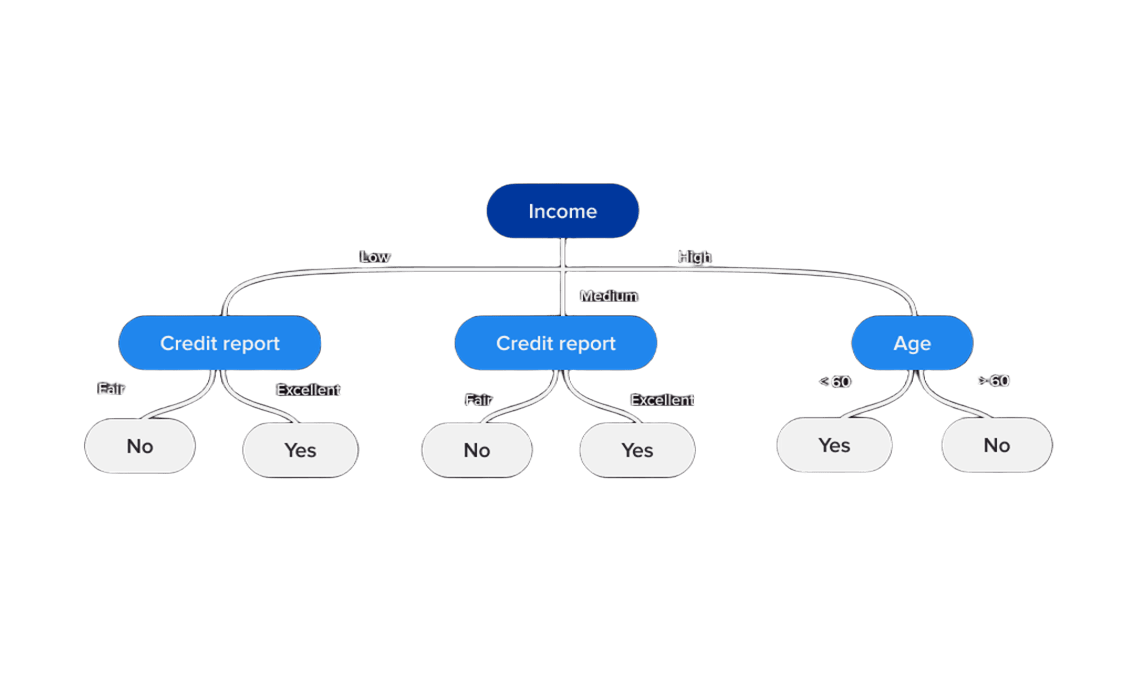
\includegraphics[height=4cm]{images/rf_example2.png}
            \end{figure}
        \end{column}
    \end{columns}
\end{frame}

\begin{frame}[c]{Análise dos Classificadores}
    \begin{columns}[c]
        \begin{column}{0.48\textwidth}
            \vspace{0.4cm}
            \begin{itemize}
                \item \textbf{Acurácia:} 
                \[
                \frac{\text{TP} + \text{TN}}{\text{TP} + \text{TN} + \text{FP} + \text{FN}}
                \]
                \item \textbf{Precisão:} 
                \[
                \frac{\text{TP}}{\text{TP} + \text{FP}}
                \]
                \item \textbf{Completeness:} 
                \[
                \frac{\text{TP}}{\text{TP} + \text{FN}}
                \]
            \end{itemize}
        \end{column}
        \begin{column}{0.48\textwidth}
            \vspace{0.4cm}
            \begin{itemize}
                \item \textbf{F1-Score:} 
                \[
                2 \cdot \frac{\text{Precisão} \cdot \text{Completeness}}{\text{Precisão} + \text{Completeness}}
                \]
                \item \textbf{AUC-ROC:} Mede sensibilidade vs. taxa de falsos positivos.
                \item \textbf{MCC:} 
                \[
                \frac{\text{TP} \cdot \text{TN} - \text{FP} \cdot \text{FN}}{\sqrt{(\text{TP} + \text{FP})(\text{TP} + \text{FN})(\text{TN} + \text{FP})(\text{TN} + \text{FN})}}
                \]
            \end{itemize}
        \end{column}
    \end{columns}
    \vspace{0.5cm}
    \begin{table}[!ht]
        \centering
        \scriptsize
        \begin{tabular}{|c|c|c|}
            \hline
            \textbf{Real} & \textbf{Sim (Detectada)} & \textbf{Não (Detectada)} \\ \hline
            Sim           & Verdadeiro Positivo (TP) & Falso Negativo (FN)      \\ \hline
            Não           & Falso Positivo (FP)      & Verdadeiro Negativo (TN) \\ \hline
        \end{tabular}
        \caption{Matriz de Confusão.}
    \end{table}
\end{frame}

\begin{frame}[c]{Análise dos Classificadores}
    \begin{columns}[c]
        \begin{column}{0.48\textwidth}
            \vspace{-0.8cm} % Ajusta o espaço vertical para começar mais acima
            \scriptsize
            \begin{table}[!ht]
                \centering
                \caption{Classificação binária - Métricas modelo KNN}
                \begin{tabular}{lccc}
                    \toprule
                    Classe & Precisão & Completeza & F1-Score \\
                    \midrule
                    0 & 0.92 & 0.88 & 0.90 \\
                    1 & 0.86 & 0.91 & 0.88 \\
                    \midrule
                    \multicolumn{3}{l}{AUC-ROC} & 0.95 \\
                    \multicolumn{3}{l}{Coeficiente de Correlação de Matthews (MCC)} & 0.78 \\
                    \bottomrule
                \end{tabular}
            \end{table}
            % \vspace{0.2cm}
            \begin{table}[!ht]
                \centering
                \caption{Classificação binária - Métricas modelo RF}
                \begin{tabular}{lccc}
                    \toprule
                    Classe & Precisão & Completeza & F1-Score \\
                    \midrule
                    0 & 0.95 & 0.90 & 0.92 \\
                    1 & 0.89 & 0.94 & 0.91 \\
                    \midrule
                    \multicolumn{3}{l}{AUC-ROC} & 0.97 \\
                    \multicolumn{3}{l}{Coeficiente de Correlação de Matthews (MCC)} & 0.84 \\
                    \bottomrule
                \end{tabular}
            \end{table}
        \end{column}
        % Coluna da direita com as imagens
        \begin{column}{0.48\textwidth}
            \centering
            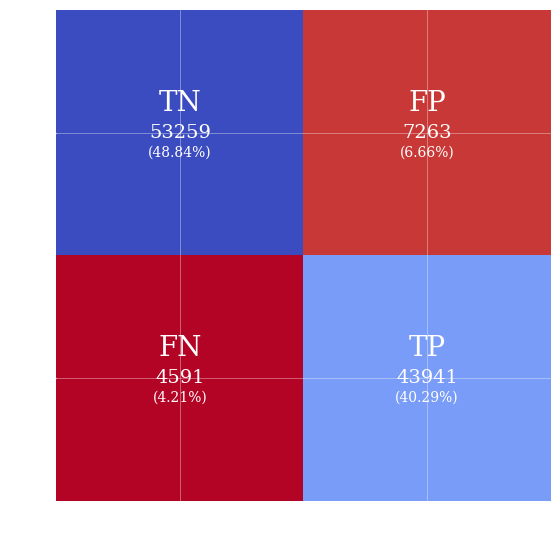
\includegraphics[width=\linewidth, height=4.2cm, keepaspectratio]{images/confusion_matrix_knn.png}
            \vspace{0.5cm}
            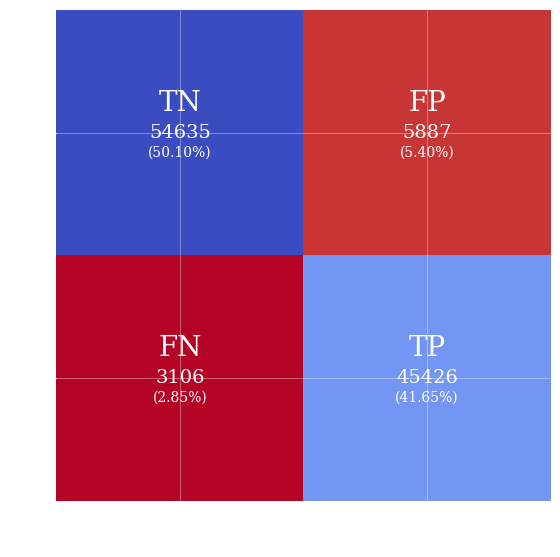
\includegraphics[width=\linewidth, height=4.2cm, keepaspectratio]{images/confusion_matrix_rf.png}
        \end{column}
    \end{columns}
\end{frame}

\begin{frame}[c]{Análise dos Classificadores}
    \begin{columns}[c]
        \begin{column}{0.42\textwidth} % Aumenta a largura da coluna da primeira imagem
            \centering
            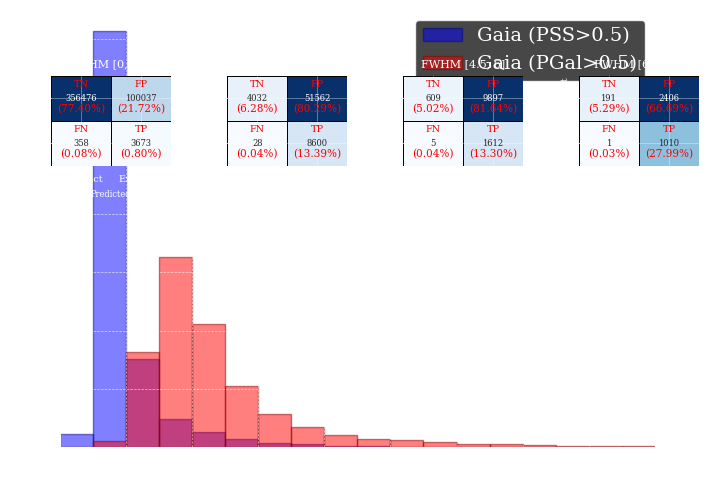
\includegraphics[width=\linewidth, height=0.5\textheight, keepaspectratio]{images/distribution_of_stars_and_galaxies_with_cm.png}
        \end{column}
        \begin{column}{0.4\textwidth} % Aumenta a largura da coluna da segunda imagem
            % \centering
            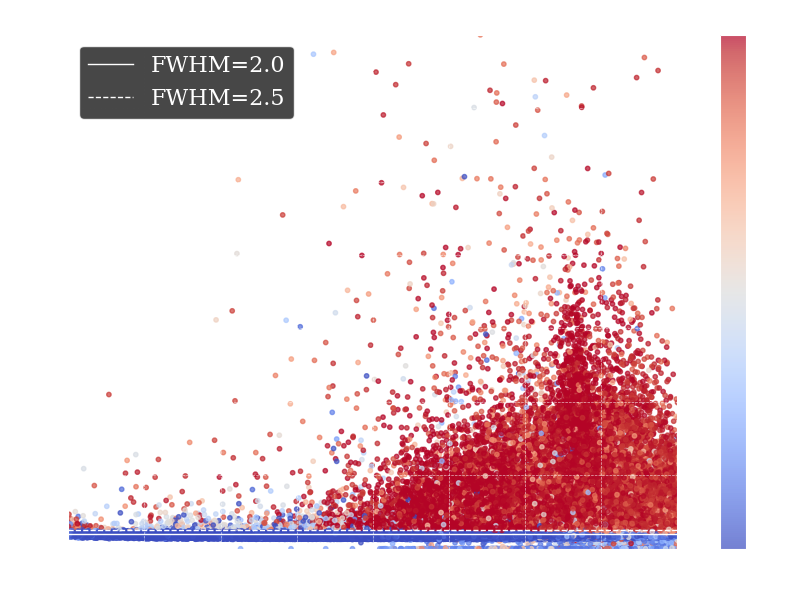
\includegraphics[width=\linewidth, height=0.5\textheight, keepaspectratio]{images/predic_colored.png}
        \end{column}
        \begin{column}{0.2\textwidth} % Reduz a largura da coluna da tabela
            \tiny
            \begin{table}[H]
                \centering
                \begin{tabular}{lc}
                    \toprule
                    Nome & RF Predição \\
                    \midrule
                    UCD3 & 0.36 \\
                    UCD1 & 0.98 \\
                    F-24 & 0.99 \\
                    UCD5 & 0.38 \\
                    F-1a & 0.11 \\
                    F-9 & 0.87 \\
                    F-5 & 0.53 \\
                    F-6 & 0.89 \\
                    F-7 & 0.70 \\
                    F-12 & 0.73 \\
                    F-11 & 0.97 \\
                    F-34 & 0.98 \\
                    F-22 & 0.93 \\
                    F-53 & 0.96 \\
                    F-51 & 0.96 \\
                    F-59 & 0.92 \\
                    \bottomrule
                \end{tabular}
            \end{table}
        \end{column}
    \end{columns}
    % \vspace{0.1cm}
        \begin{splusbox}{\scriptsize}
            \scriptsize
            \begin{itemize}
                \item \textbf{Total de objetos:} 1.803.561.
                \item \textbf{Extensos:} 1.411.803 (78,28\%). Deles 311.846 (17,29\%) com $FWHM < 2.5$ pixels.
            \end{itemize}
        \end{splusbox}
\end{frame}

\begin{frame}[c]{Redshifts Fotométricos}
    Redshifts fotométricos são estimativas baseadas em fotometria multibanda. 
    \begin{equation}
        v_\text{res} = c \cdot z = H_0 \cdot D,
    \end{equation}

    \begin{columns}
        \begin{column}{0.46\linewidth}
            \centering
            \scriptsize
            \textbf{Modelo Treinado}
            \begin{itemize}
                \item Photo-z de \textit{Lima et al. 2022}. 
                \item De 29000926, \textbf{290637} sem estimativa.
                \item $0.002 \leq z \leq 0.5$ ; $15 \leq r_{APER\_6} \leq 21$.
                \item Amostra final: 12.296 objetos.
                \item Treinamento com 66 cores (\texttt{APER\_6}).
                \item Divisão da amostra: 80\% treino, 20\% teste.
                \item Regressão com Random Forest (RF).
            \end{itemize}
        \end{column}
        \begin{column}{0.46\linewidth}
            \begin{figure}
                \centering
                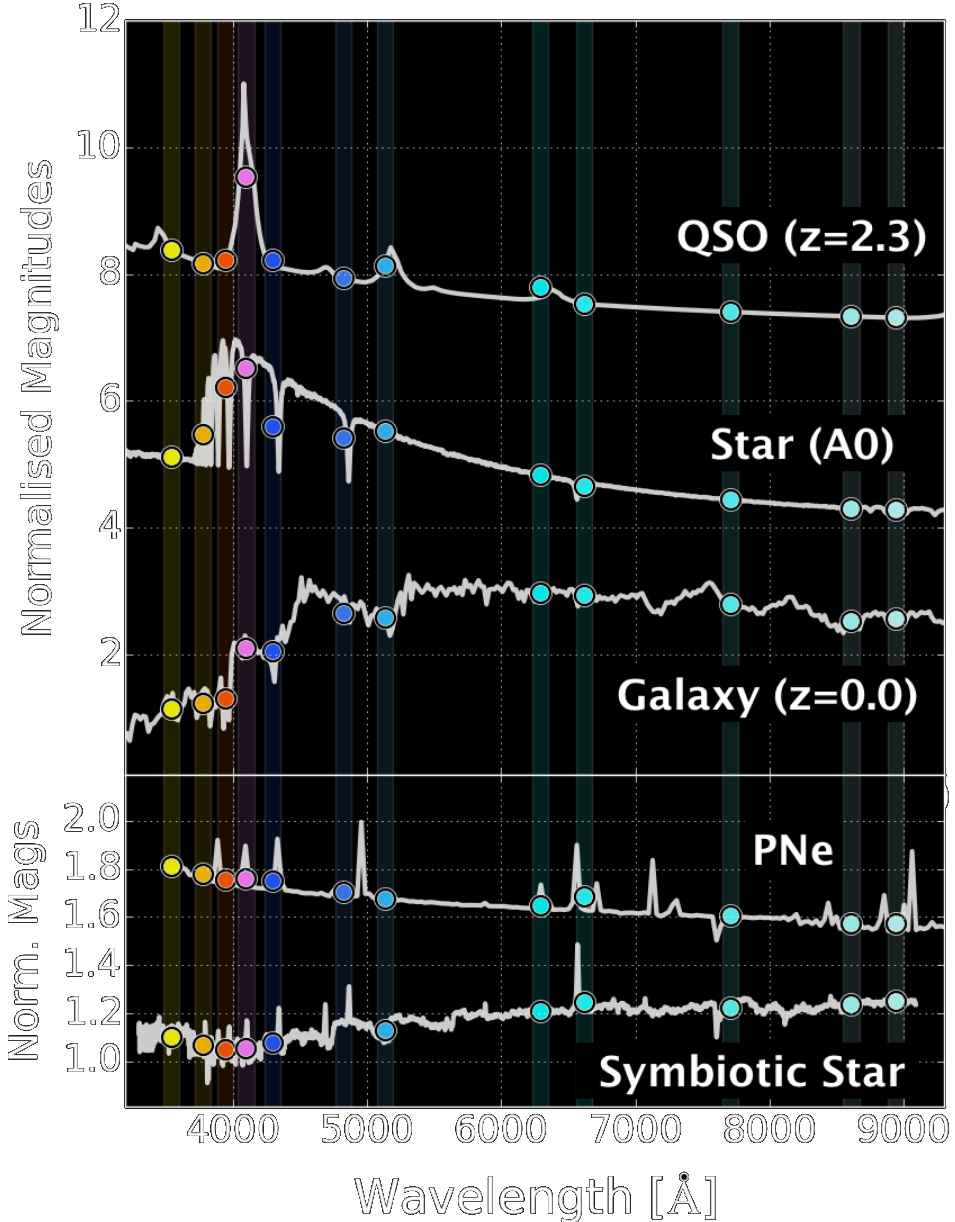
\includegraphics[height=4.5cm]{script/images/splus_spectra_sed.png}
                \caption{Adaptado de Mendes de Oliveira et al. (2019).}
            \end{figure}
        \end{column}
    \end{columns}
\end{frame}

\begin{frame}[c]{Redshifts Fotométricos}
    \vspace{0.5cm}
    \begin{figure}
        \centering
        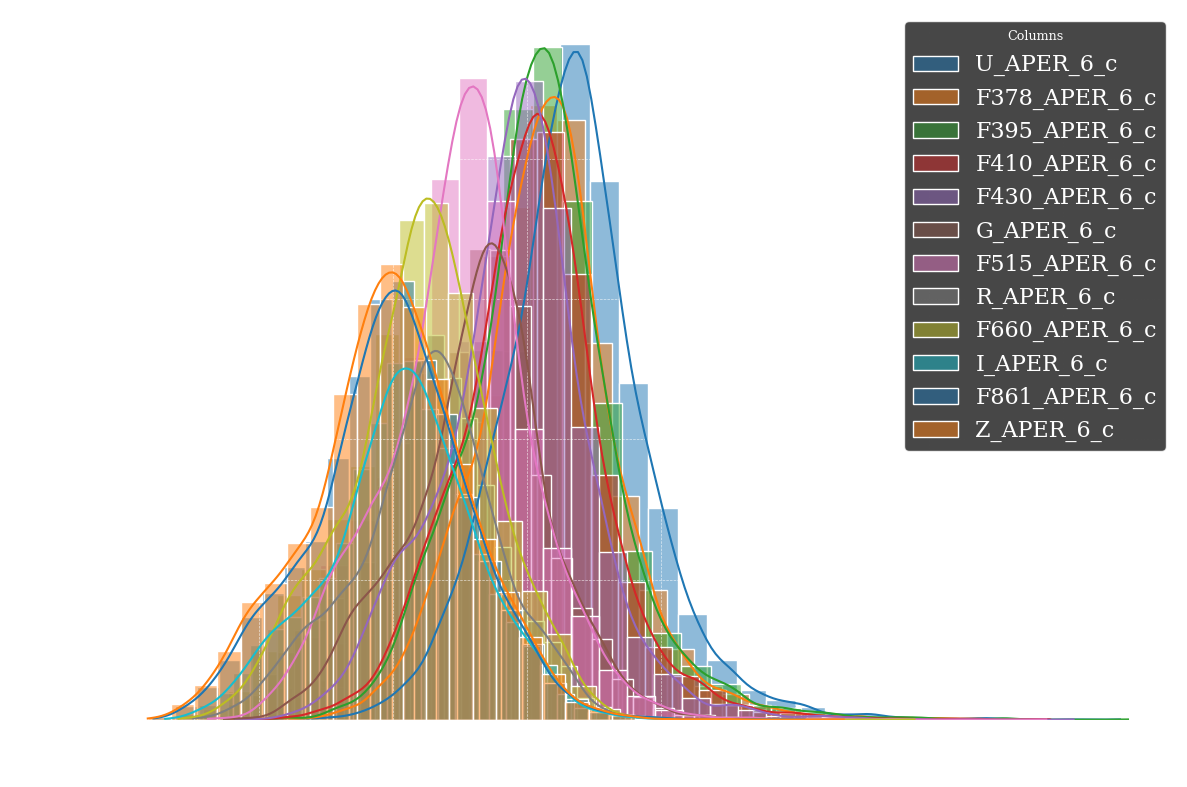
\includegraphics[width=0.8\linewidth, height=6cm, keepaspectratio]{images/overlaid_histogram_mags_aper_6_c.png}
        \caption{Distribuição magnitudes na amostra de treino \textit{photo\_z}.}
    \end{figure}
\end{frame}

\begin{frame}[c]{Redshifts Fotométricos}
    \begin{columns}[c]
        \begin{column}{0.32\linewidth}
            \begin{figure}
                \centering
                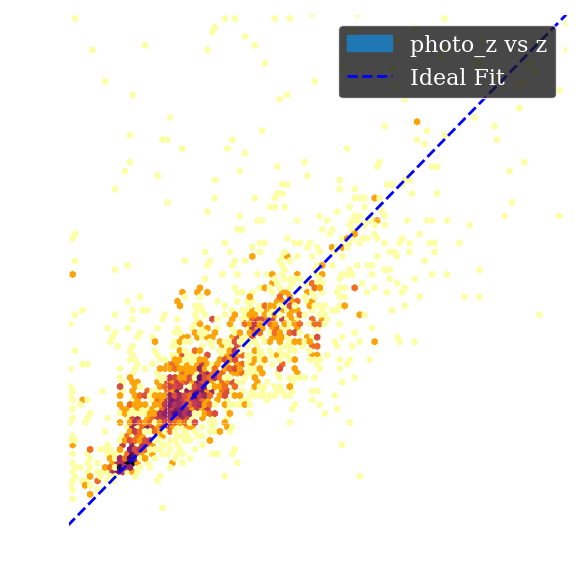
\includegraphics[width=\linewidth]{images/photo_z_test.png}
            \end{figure}
        \end{column}
        \begin{column}{0.32\linewidth}
            \begin{figure}
                \centering
                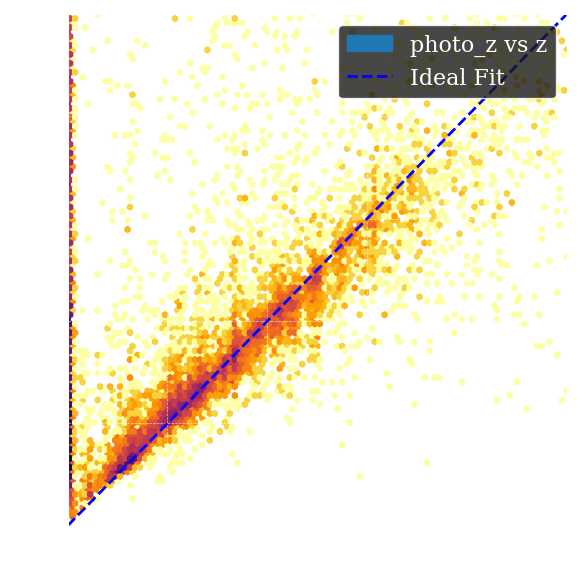
\includegraphics[width=\linewidth]{images/photo_z.png}
            \end{figure}
        \end{column}
        \begin{column}{0.32\linewidth}
            \begin{figure}
                \centering
                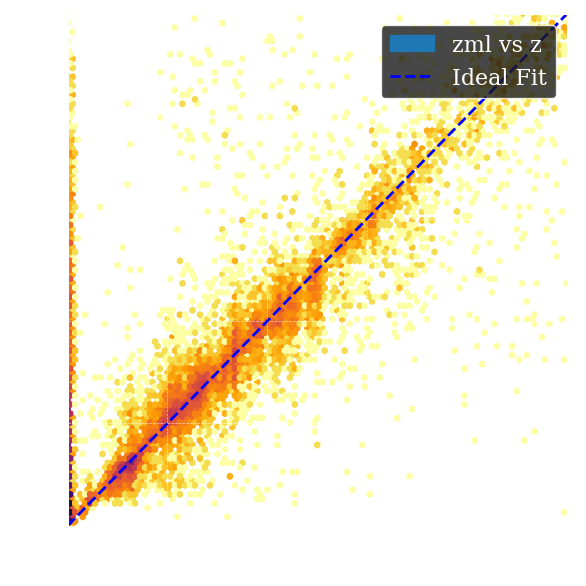
\includegraphics[width=\linewidth]{images/zml.png}
            \end{figure}
        \end{column}
    \end{columns}
    % \vspace{0.5cm}
    \begin{splusbox}{}
        \tiny
        \begin{itemize}
            \item \textbf{EQR =} 0.05
            \item \textbf{$R^2$ =} 0.6
            \item \textbf{$\sigma_{NMAD}$ =} 0.03
        \end{itemize}
    \end{splusbox}
\end{frame}

\begin{frame}[c]{Redshifts Fotométricos}
    \begin{columns}[c]
        \begin{column}{0.7\linewidth}
            \begin{figure}
                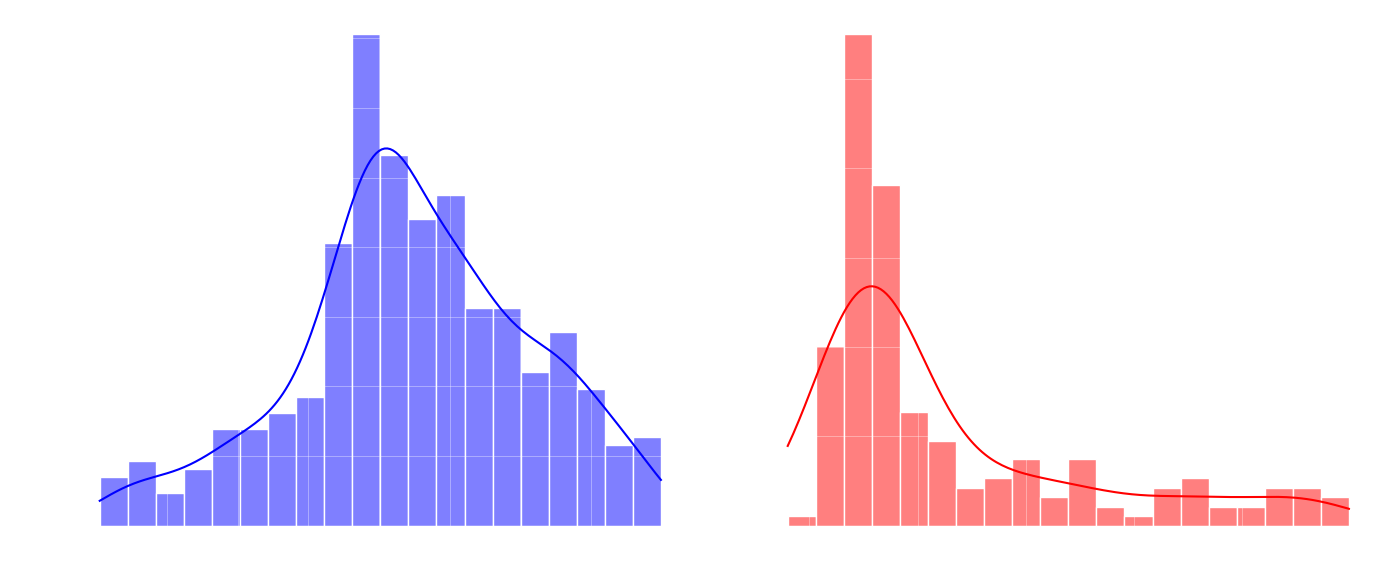
\includegraphics[width=\linewidth]{images/z_zml_distribution.png}
            \end{figure}
        \end{column}
        \begin{column}{0.25\linewidth}
            \begin{table}[!ht]
                \centering
                \scriptsize
                \begin{tabular}{lccc}
                    \toprule
                    Nome & \textit{$z_{phot}$} & \textit{zml} & \textit{$z_{spec}$}\\
                    \midrule
                    UCD3 & 0.07 & 0.03 & 0.0053\\
                    UCD1 & 0.09 & 0.08 & 0.0052\\
                    F-24 & 0.08 & 0.04 & 0.0062\\
                    UCD5 & 0.03 & 0.04 & 0.0045\\
                    F-1a & 0.21 & -- & 0.0042\\
                    F-9 & 0.09 & 0.07 & 0.0058\\
                    F-5 & 0.06 & -- & 0.0057\\
                    F-6 & 0.10 & -- & 0.0037\\
                    F-7 & 0.19 & 0.16 & 0.0050\\
                    F-12 & 0.07 & -- & 0.0055\\
                    F-11 & 0.10 & -- & 0.0059\\
                    F-34 & 0.07 & -- & 0.0054\\ 
                    F-22 & 0.09 & 0.06 & 0.0034\\
                    F-53 & 0.31 & -- & 0.0020\\
                    F-51 & 0.10 & -- & 0.0041\\
                    F-59 & 0.06 & -- & 0.0060\\
                    \midrule
                \end{tabular}
            \end{table}
        \end{column}
    \end{columns}
\end{frame}




% \begin{frame}[c]{Redshifts Fotométricos}

% \begin{frame}[c]{Redshifts Fotométricos}
%     \begin{columns}[c]
%         \begin{column}{0.32\linewidth}
%             \begin{figure}
%                 \centering
%                 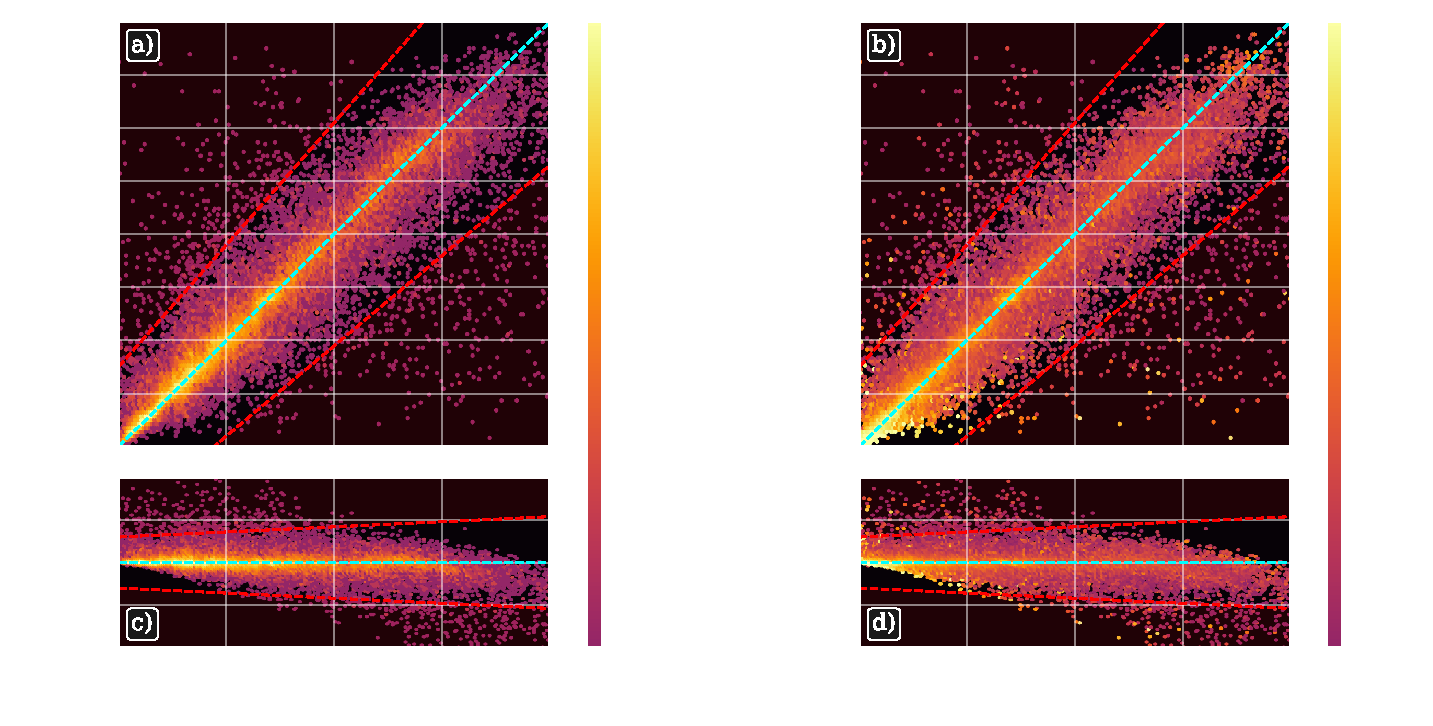
\includegraphics[width=\linewidth]{images/results_scatterplot_residuals.pdf}
%                 \caption{Resíduos entre $z_\text{phot}$ e $z_\text{spec}$.}
%             \end{figure}
%         \end{column}
%         \begin{column}{0.32\linewidth}
%             \begin{figure}
%                 \centering
%                 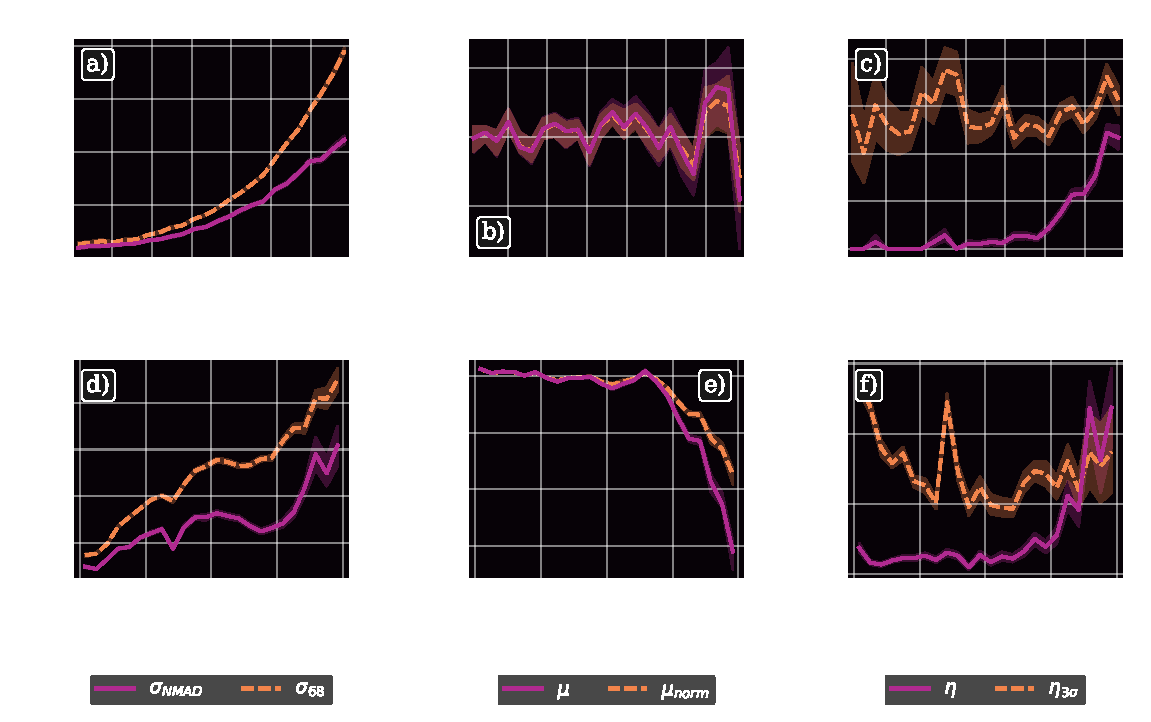
\includegraphics[width=\linewidth]{images/results_spe_metrics.pdf}
%                 \caption{Métricas de desempenho do modelo.}
%             \end{figure}
%         \end{column}
%         \begin{column}{0.32\linewidth}
%             \begin{figure}
%                 \centering
%                 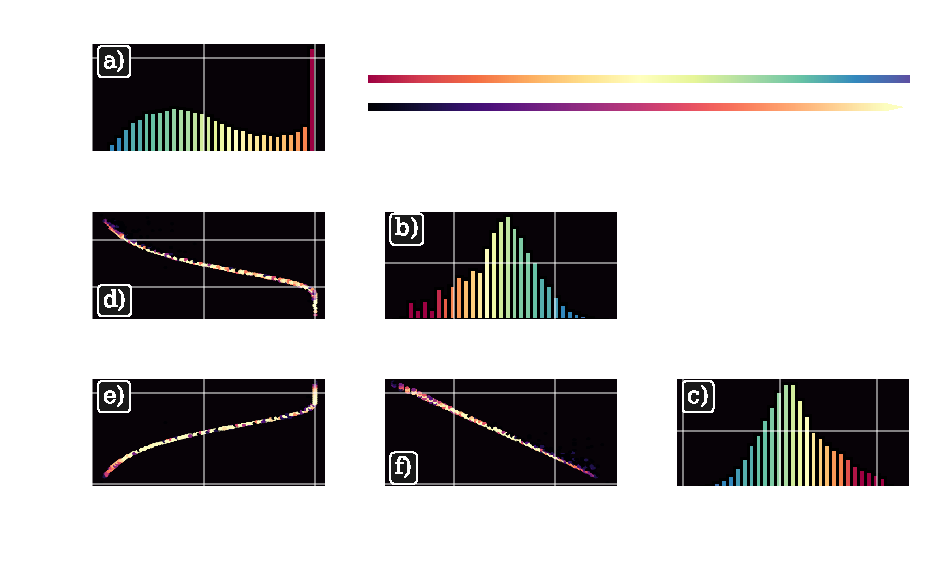
\includegraphics[width=\linewidth]{images/results_pdf_metrics_triangle.pdf}
%                 \caption{Distribuição das PDFs geradas.}
%             \end{figure}
%         \end{column}
%     \end{columns}
% \end{frame}


% % Slide 8: Conclusões
% \begin{frame}[c]{Conclusões}
%     \begin{splusbox}{Resumo}
%         \begin{itemize}
%             \item Modelo RF apresentou melhor desempenho em comparação ao KNN.
%             \item Classificação baseada em FWHM é eficiente para separar objetos compactos e extensos.
%             \item Tratamento de valores faltantes foi essencial para garantir consistência nos resultados.
%         \end{itemize}
%     \end{splusbox}
% \end{frame}




% \section{aaaa}
% \begin{frame}[c]{Criando o catálogo para treinamento}
%     \begin{splusbox}{Crossmatches espectroscópicos}
%         \small
%         Busca radial (RA, DEC) com raio de 2" em torno de cada objeto do SPLUS
%     \end{splusbox}
%     \begin{splusbox}{Crossmatches fotométricos}
%         \small
%         \begin{columns}[t]
%             \begin{column}{0.29\textwidth}
%                GALEX \textcolor{LightGray}{(II/335/galex\_ais)}:
%                \begin{itemize}
%                     \item Busca radial com raio de 2"
%                 \end{itemize}
%             \end{column}
%             \begin{column}{0.29\textwidth}
%                 VHS \textcolor{LightGray}{(II/367/vhs\_dr5)}:
%                 \begin{itemize}
%                     \justifying
%                     \item Busca radial com raio de 1"
%                     \item Conversão de magnitudes Vega para AB
%                 \end{itemize}
%             \end{column}
%             \begin{column}{0.29\textwidth}
%                 unWISE \textcolor{LightGray}{(II/363/unwise)}:
%                 \begin{itemize}
%                     \justifying
%                     \item Busca radial com raio de 1"
%                     \item Cálculo das magnitudes e erros
%                     \item Conversão de magnitudes Vega para AB
%                 \end{itemize}
%             \end{column}
%         \end{columns}
%     \end{splusbox}
% \end{frame}

% \begin{frame}[c]{Pré-processamento}
%     \begin{columns}[c]
%         \begin{column}{0.56\linewidth}
%             \vspace{0.2cm}
%             \begin{table}
%                 \centering
%                 \label{tab:constraints}
%                   \begin{tabular}{@{}ll@{}}
%                       \toprule
%                       \textbf{Variable}        & \textbf{Constraints}                              \\ \midrule
%                       \texttt{r\_auto}         & {[}14, 21{]}                                      \\
%                       \texttt{nDet\_PStotal}   & $\geqslant$ 1                                     \\
%                       \texttt{SEX\_FLAGS\_DET} & {[}0, 3{]}                                        \\ \midrule
%                       \texttt{z}               & {[}0.002, 0.8{]}                                    \\
%                       \texttt{e\_z}            & $\leqslant$ 0.002                                 \\
%                       \texttt{f\_z}            & not \ttt{REMOVE}                                  \\
%                       \texttt{class\_spec}     & \ttt{GALAXY}, \ttt{SUPERNOVAE} or \ttt{AGN}       \\
%                       Separation               & $\leqslant$ 1''                                   \\ \bottomrule
%                   \end{tabular}
%               \end{table}
%         \end{column}
%         %
%         %\hspace*{-2cm}
%         \begin{column}{0.36\linewidth}
%             \begin{splusbox}{}
%                 \begin{itemize}
%                     \justifying
%                     \item Galáxias
%                     \item Nem muito fracas, nem muito brilhantes
%                     \item Com boa fotometria
%                     \item Com redshifts de boa qualidade e entre 0.002 e 0.8
%                 \end{itemize}
%             \end{splusbox}
%         \end{column}
%     \end{columns}
% \end{frame}

% \begin{frame}[c]{Pré-processamento}
%     \begin{figure}
%         \centering
%         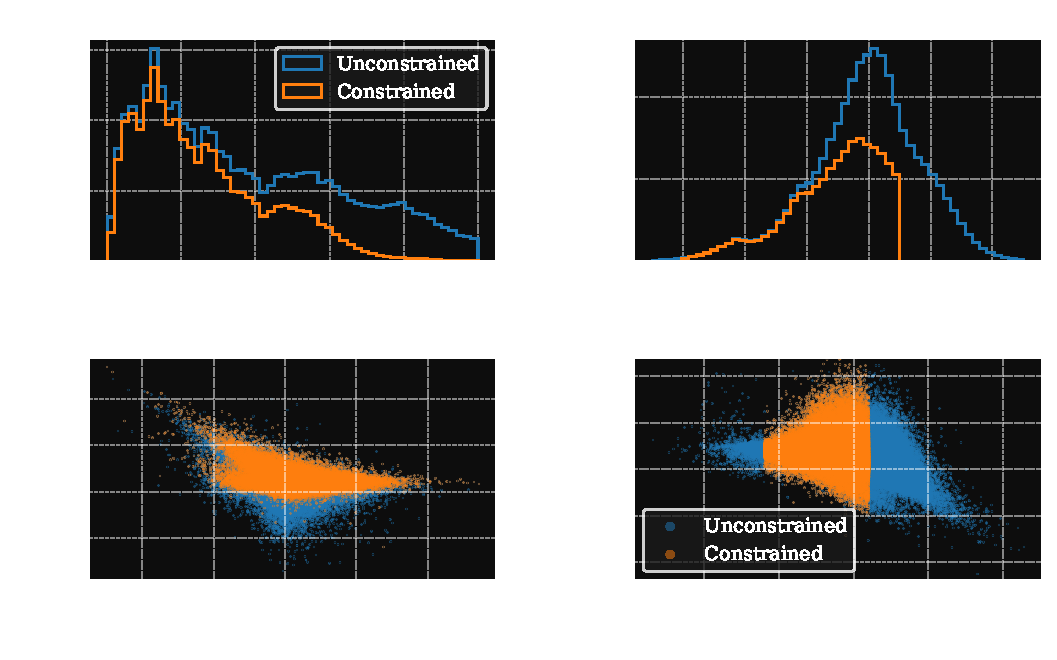
\includegraphics[height=7cm]{script/images/constraints_effect.pdf}
%     \end{figure}
% \end{frame}

% \begin{frame}[c]{Pesos por objeto}
%     A distribuição de spec-zs da amostra de treino é diferente da distribuição esperada no universo.
%     \begin{equation*}
%         P(y|\mathcal{D}) = \int P(y,\theta|\mathcal{D}) \text{d}\theta = \int P(y|\theta, \mathcal{D}) P(\theta|D) \text{d}\theta
%     \end{equation*}
%     % \hspace{0.5cm}
%     \begin{splusbox}{}
%         Os resultados para $y$ dependem dos dados $\mathcal{D}$, então o conjunto de treinamento pode introduzir viéses.
%     \end{splusbox}
% \end{frame}

% \begin{frame}[c]{Pesos por objeto}
%     Assumimos que a distribuição de $z_\text{spec}$ é conhecida para surveys limitados por fluxo, e modelamos esta distribuição como função da magnitude usando a amostra do COSMOS2020 (Weaver et al., 2022) e uma função Weibull de dois parâmetros $l$ e $k$.

%     \begin{figure}
%         \centering
%         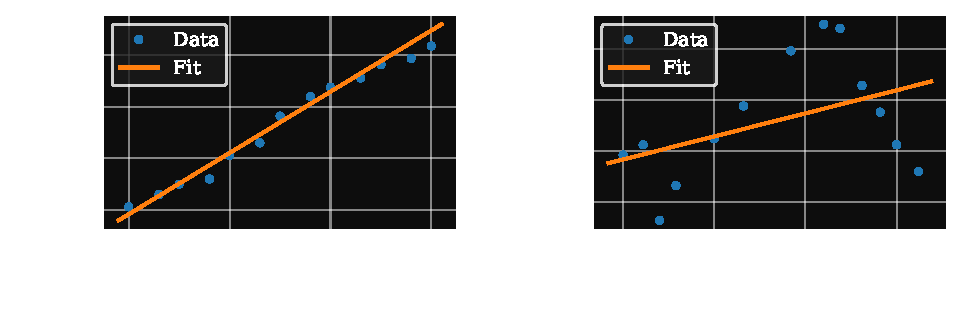
\includegraphics[width=\linewidth]{script/images/laerte_fit.pdf}
%     \end{figure}
% \end{frame}

% \begin{frame}[c]{Pesos por objeto}
%     \begin{figure}
%         \centering
%         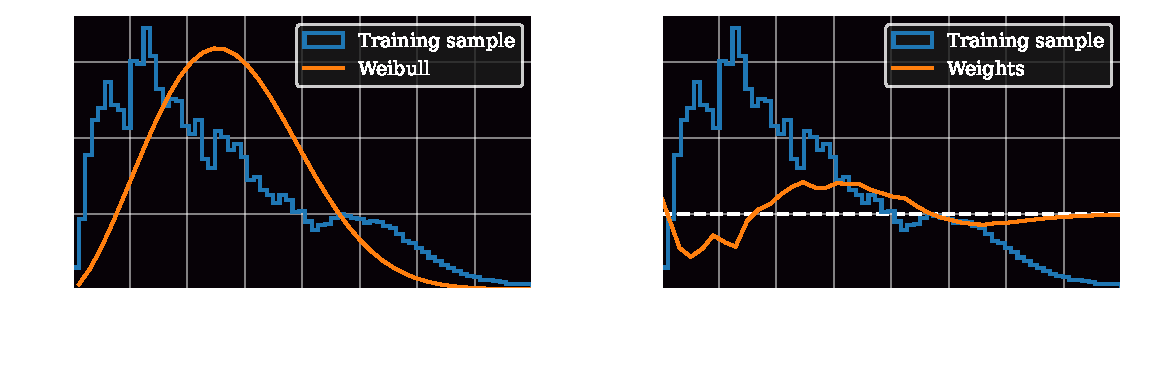
\includegraphics[width=\linewidth]{script/images/weights_vs_specz.pdf}
%     \end{figure}

%     Com essa abordagem, cada objeto contribui de forma diferente no treinamento do modelo
% \end{frame}

% \section{Metodologia}
%     % \begin{tikzpicture}[overlay, remember picture]
%     %     % Image 1 at specified position
%     %     \node at (3.75, 1.5) {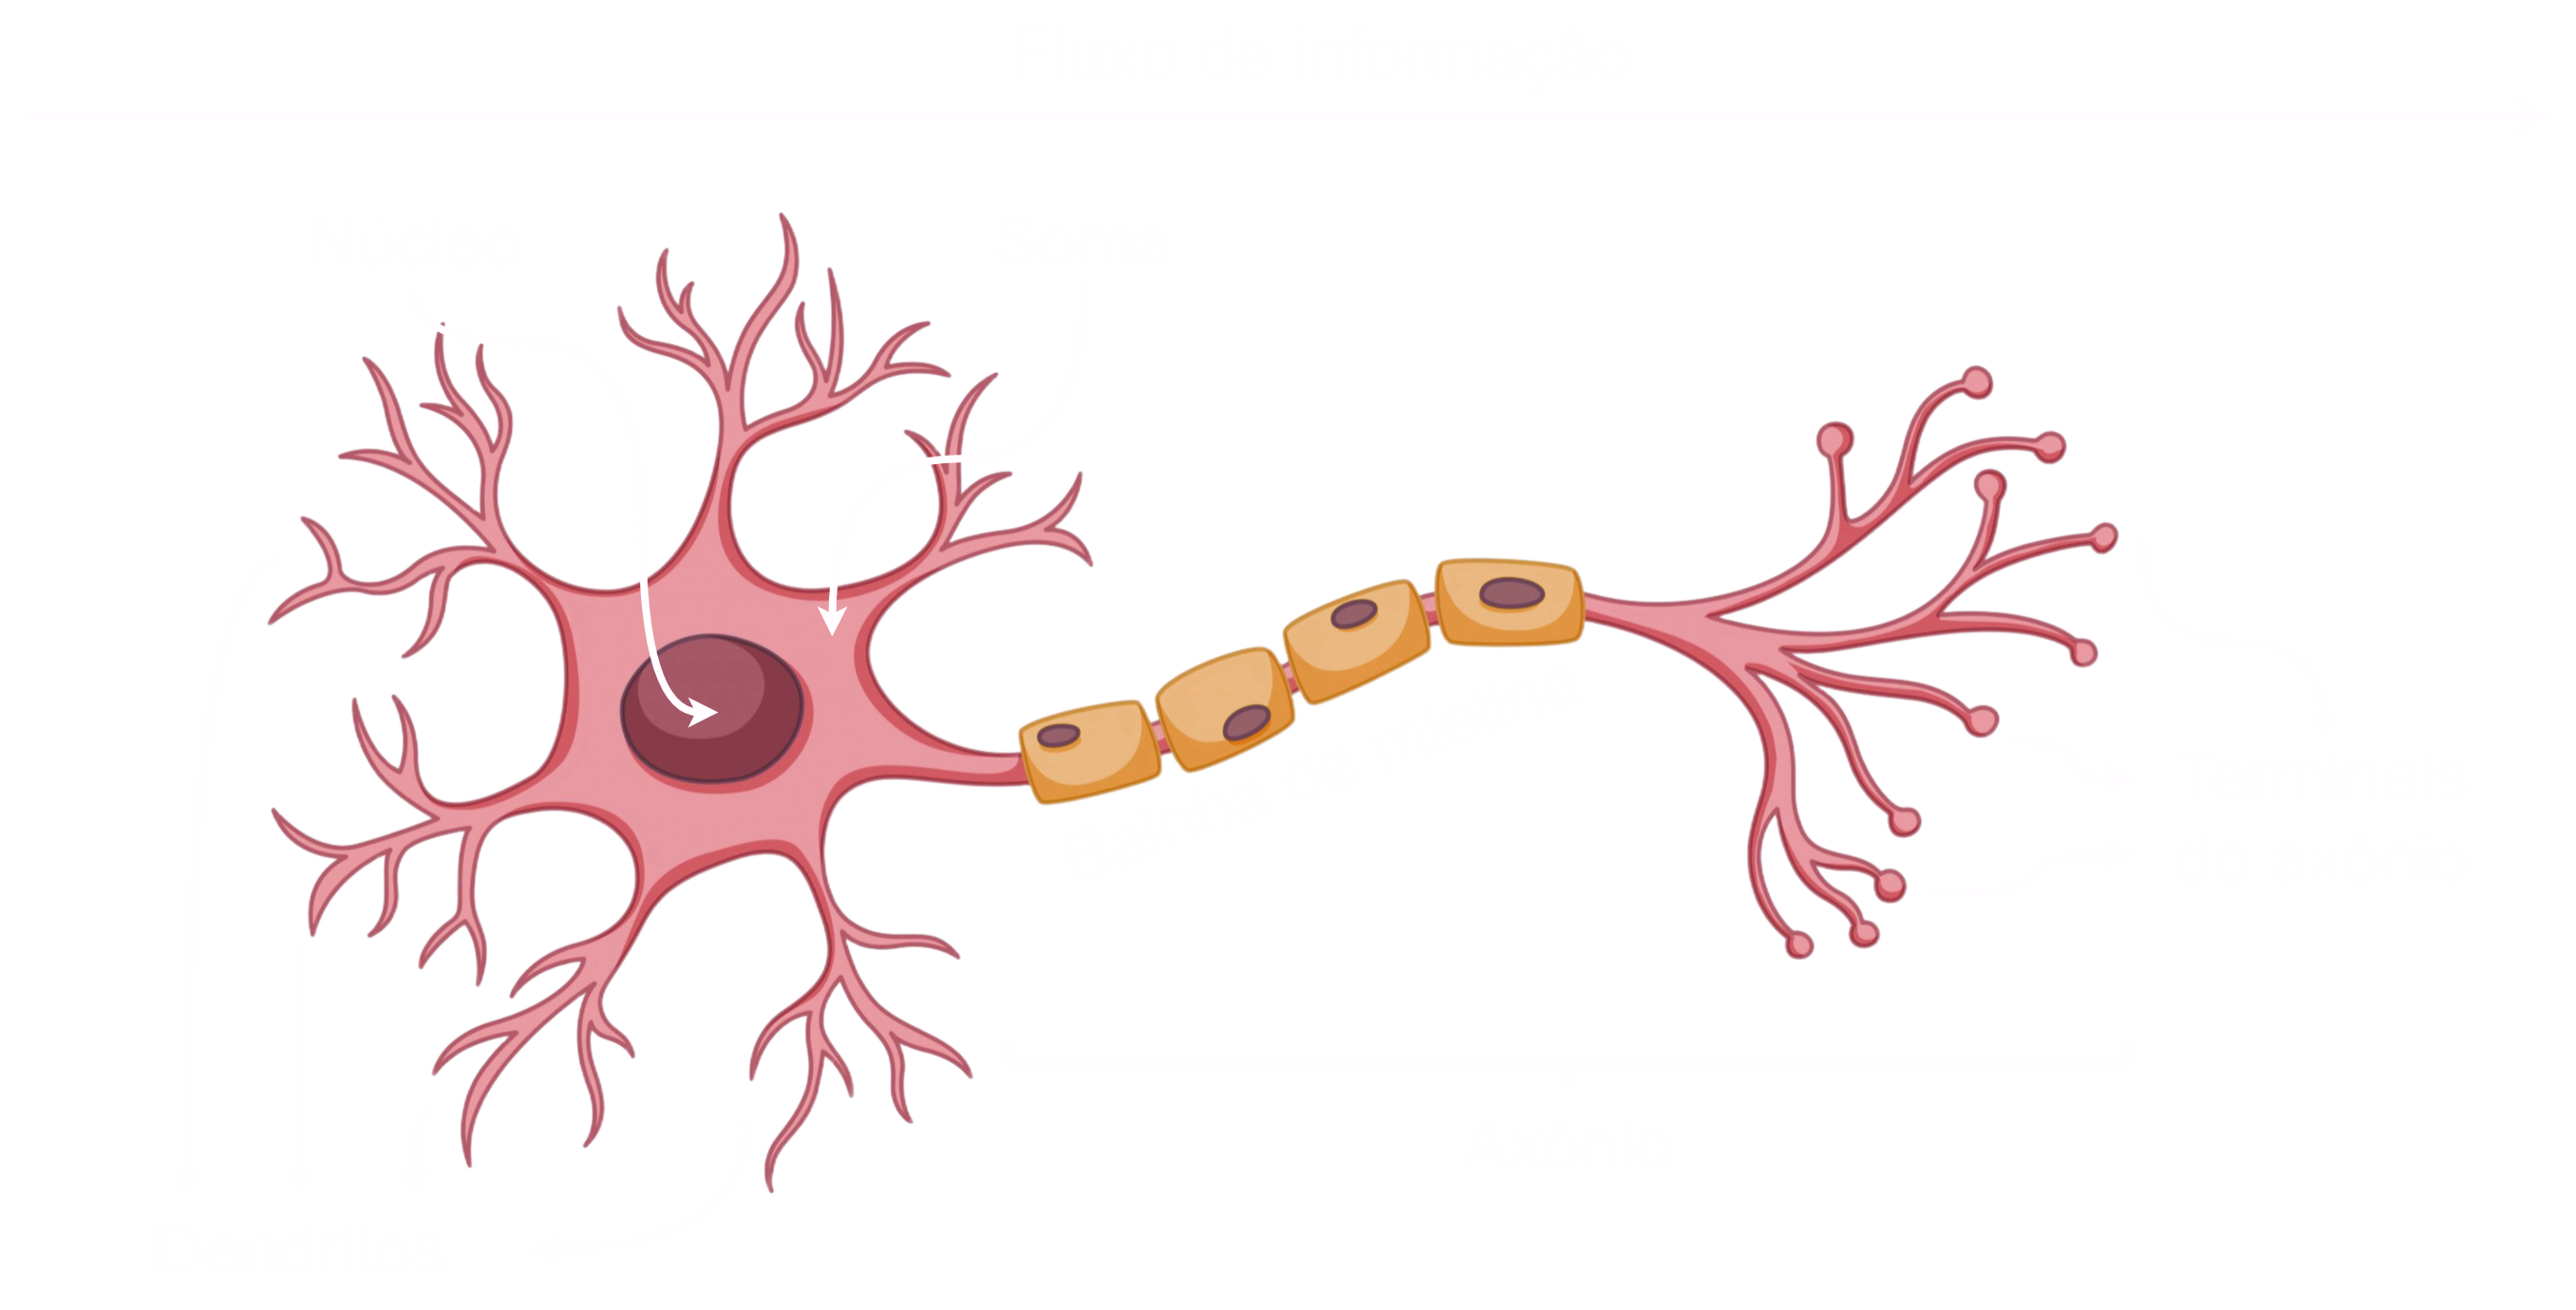
\includegraphics[height=4cm]{script/images/neuron_bio.png}};
        
%     %     % Image 2 at specified position
%     %     \node at (11, -1.5) {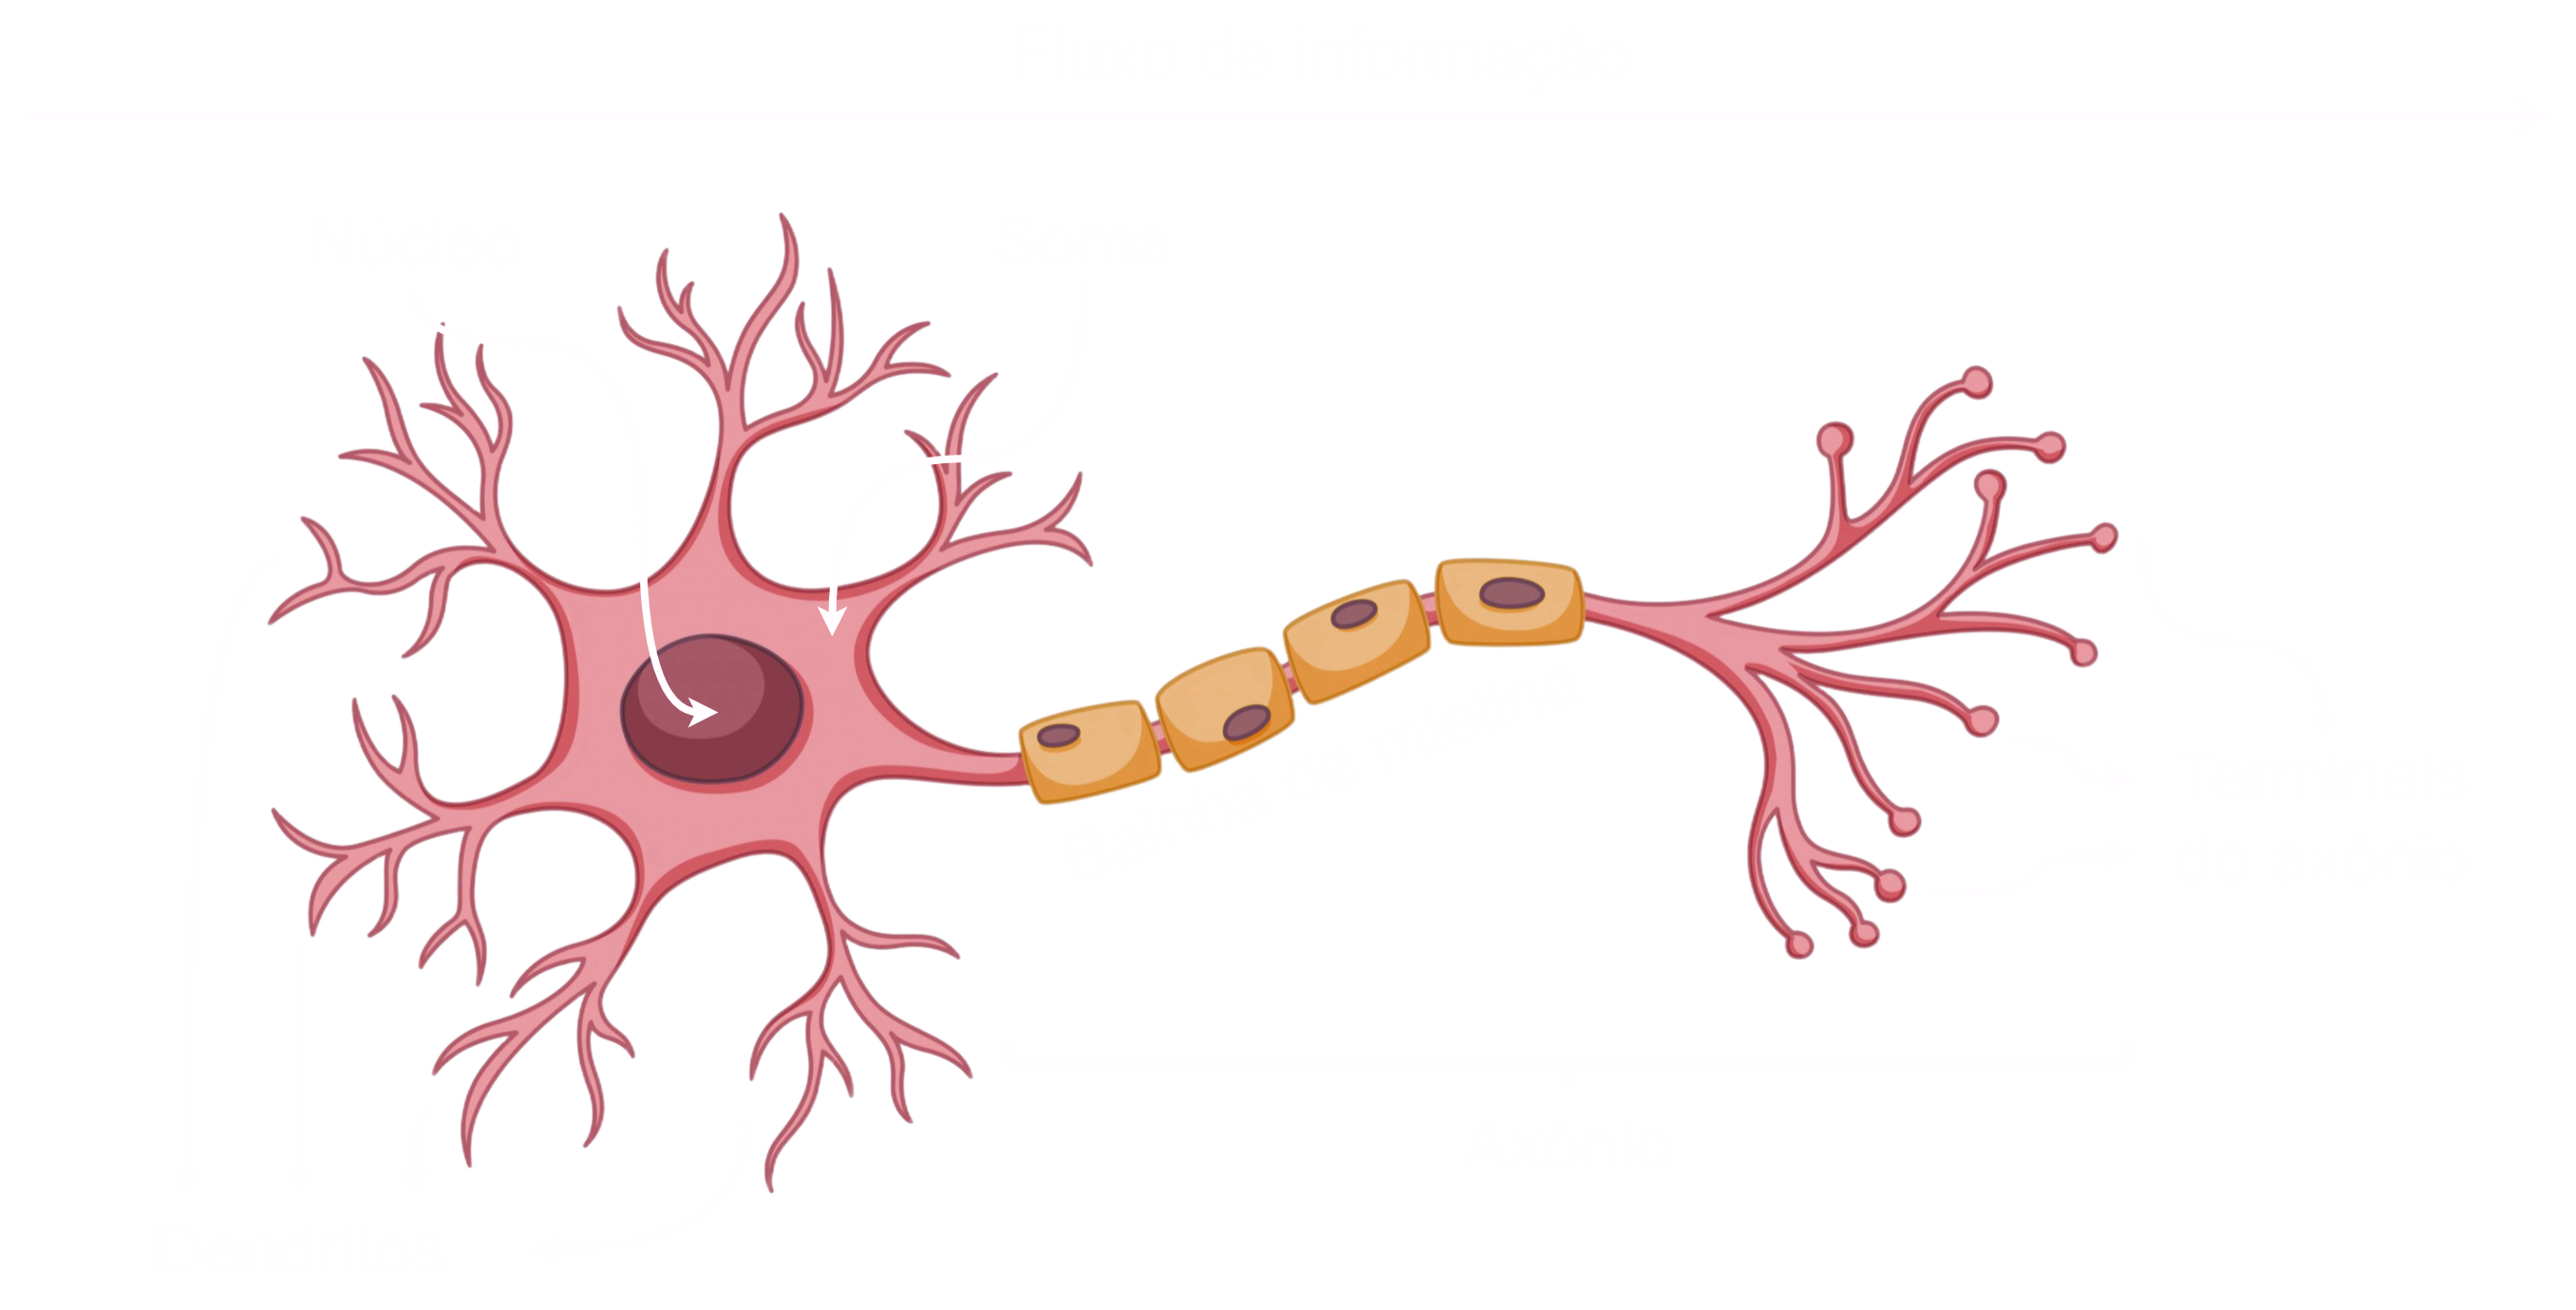
\includegraphics[height=4cm]{script/images/neuron_bio.png}};
%     % \end{tikzpicture}

% \begin{frame}[c]{Redes neurais}
%     \begin{figure}
%         \centering
%         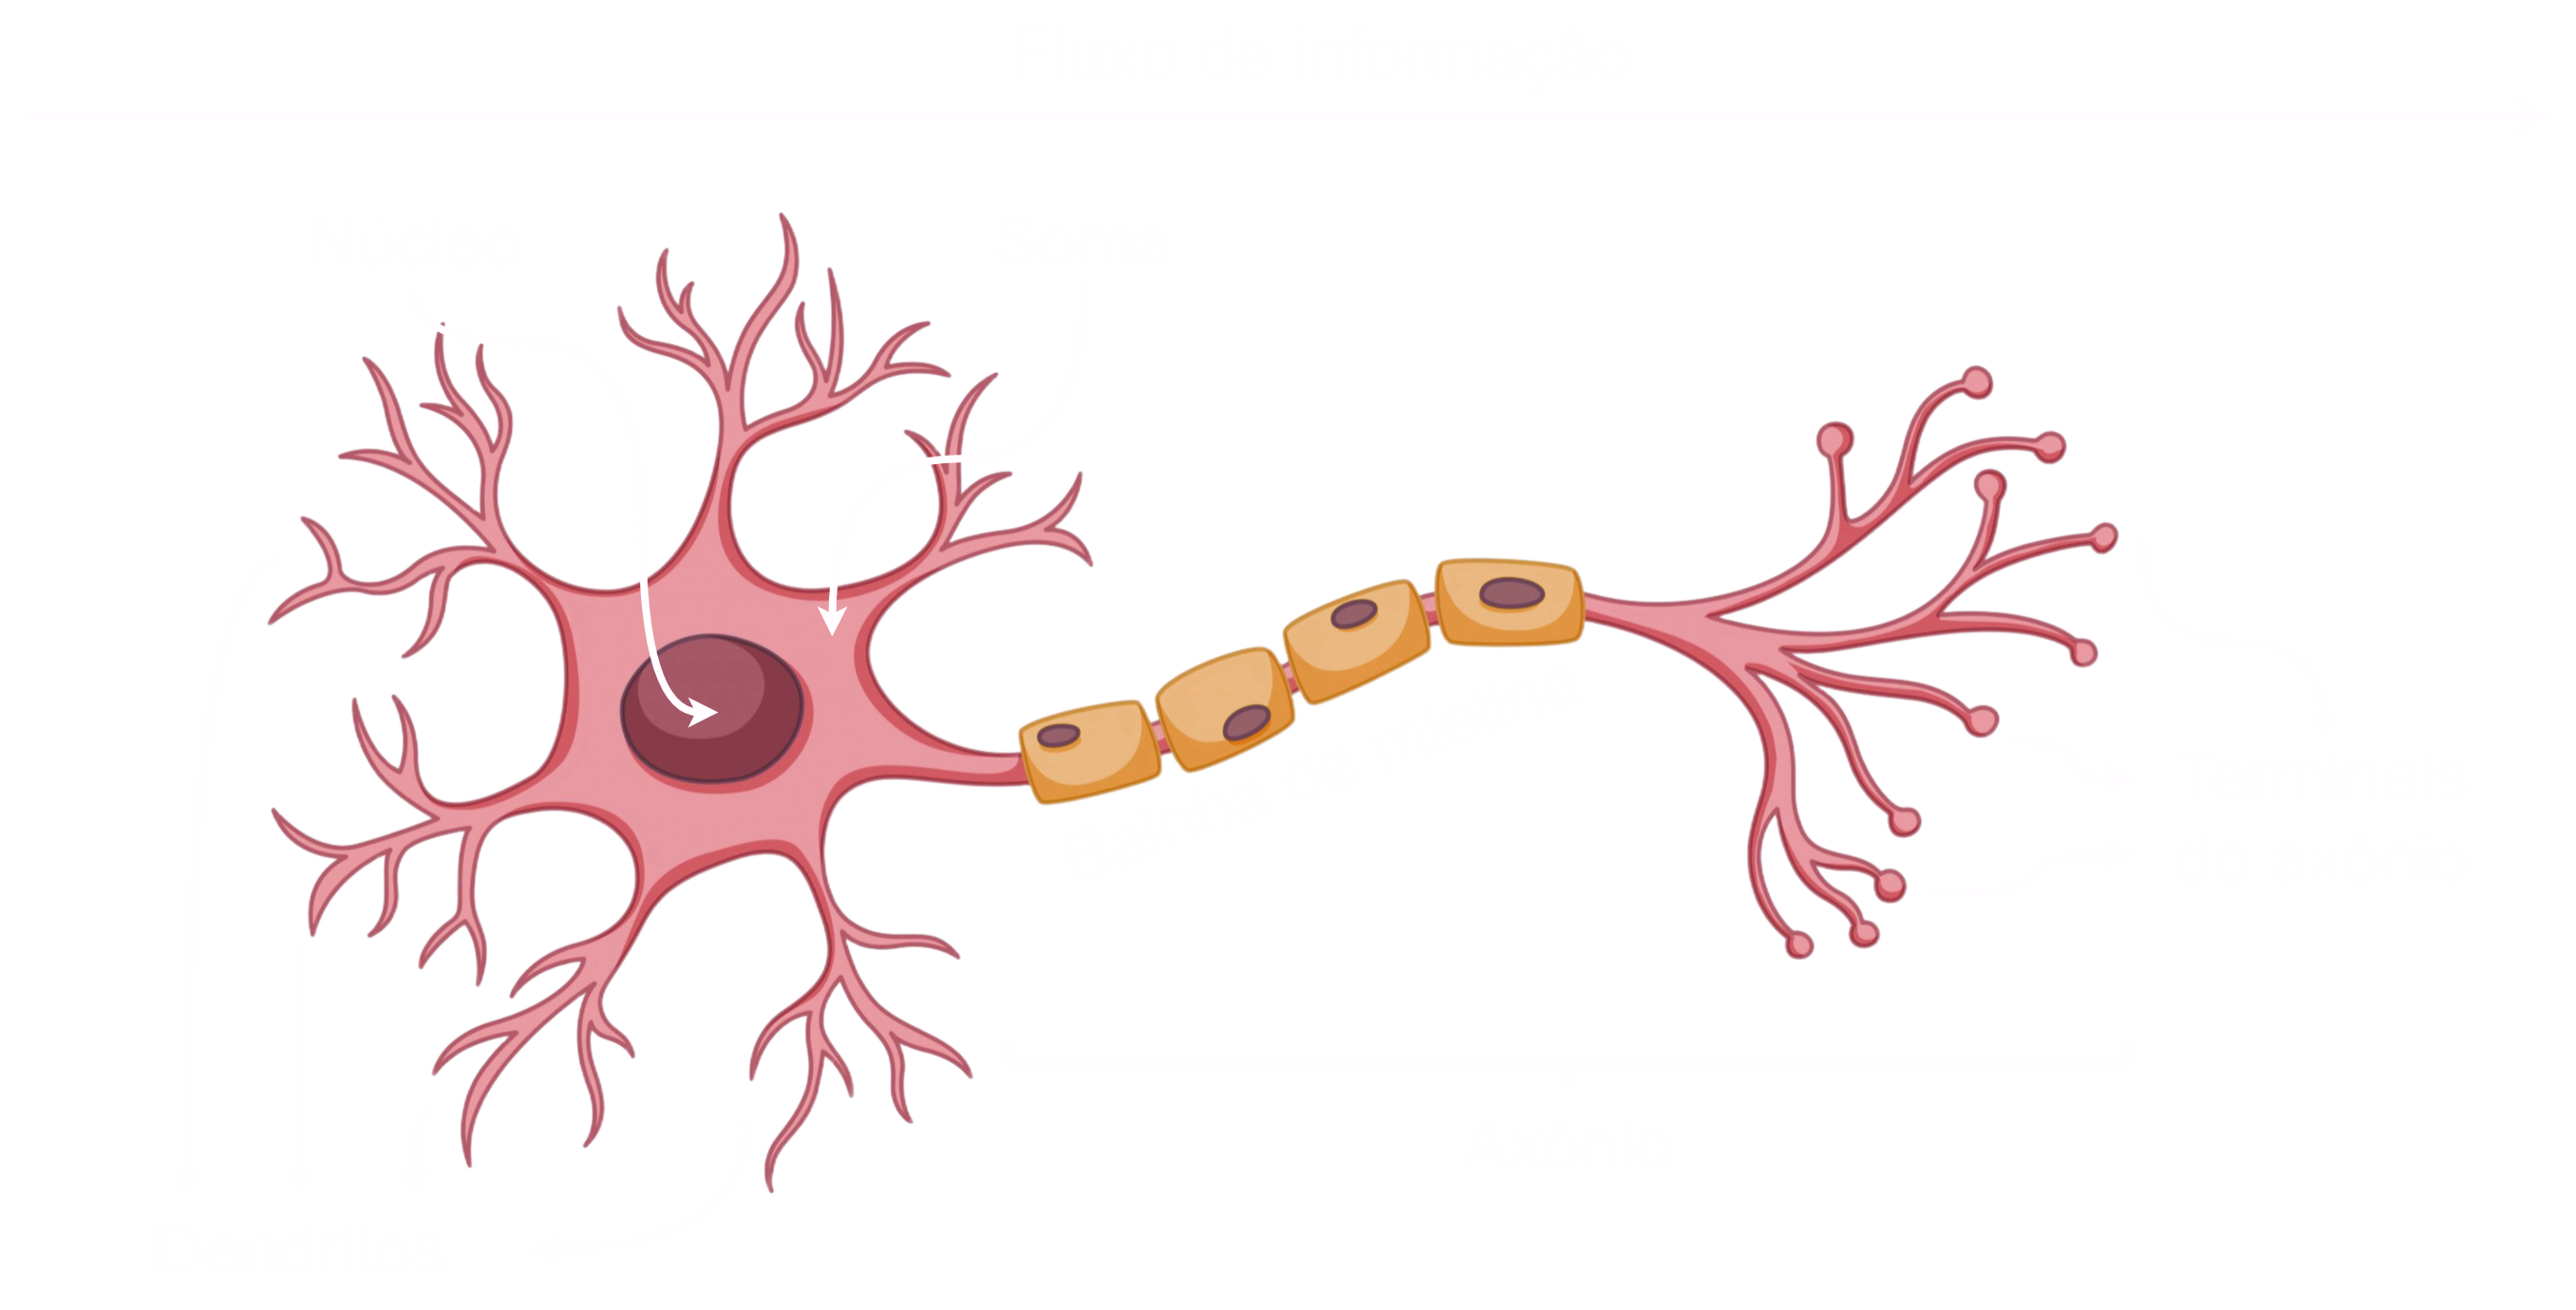
\includegraphics[height=6cm]{script/images/neuron_bio.png}
%     \end{figure}
% \end{frame}

% \begin{frame}[c]{Redes neurais}
%     \begin{figure}
%         \centering
%         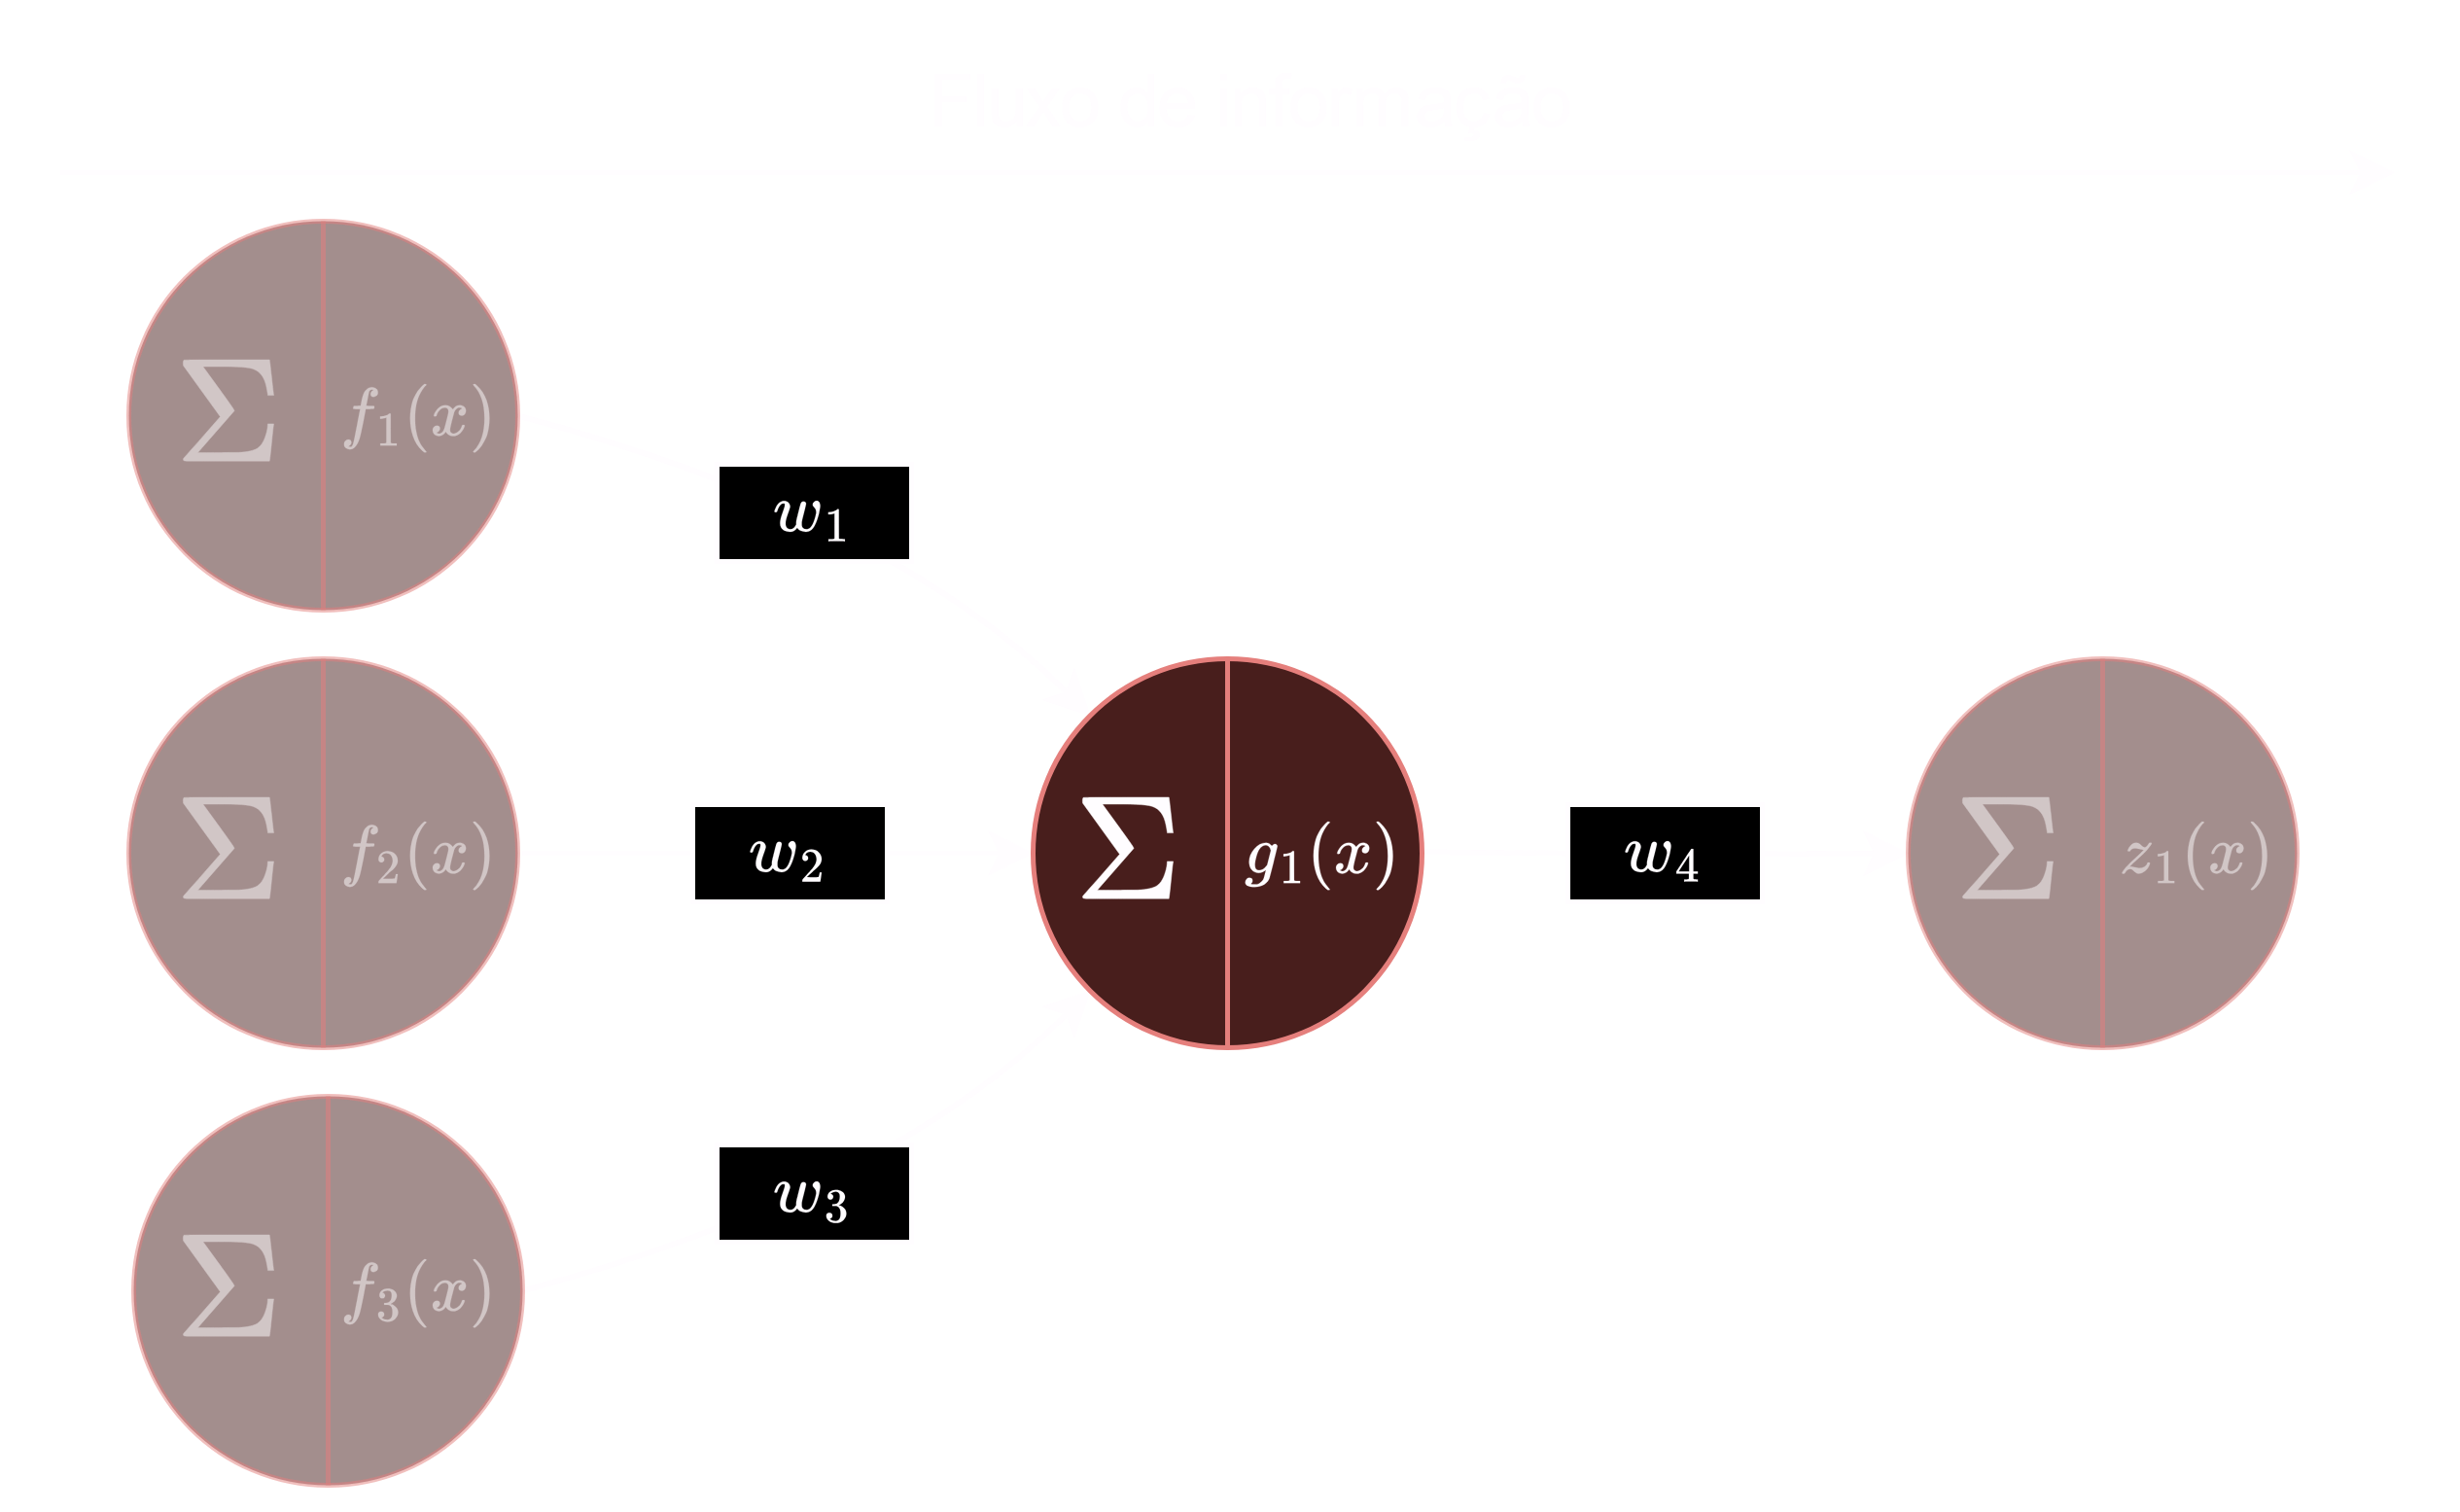
\includegraphics[height=6cm]{script/images/neuron_ml_pesos.png}
%     \end{figure}
% \end{frame}

% % \begin{frame}[c]{Redes neurais}
% %     \begin{figure}
% %         \centering
% %         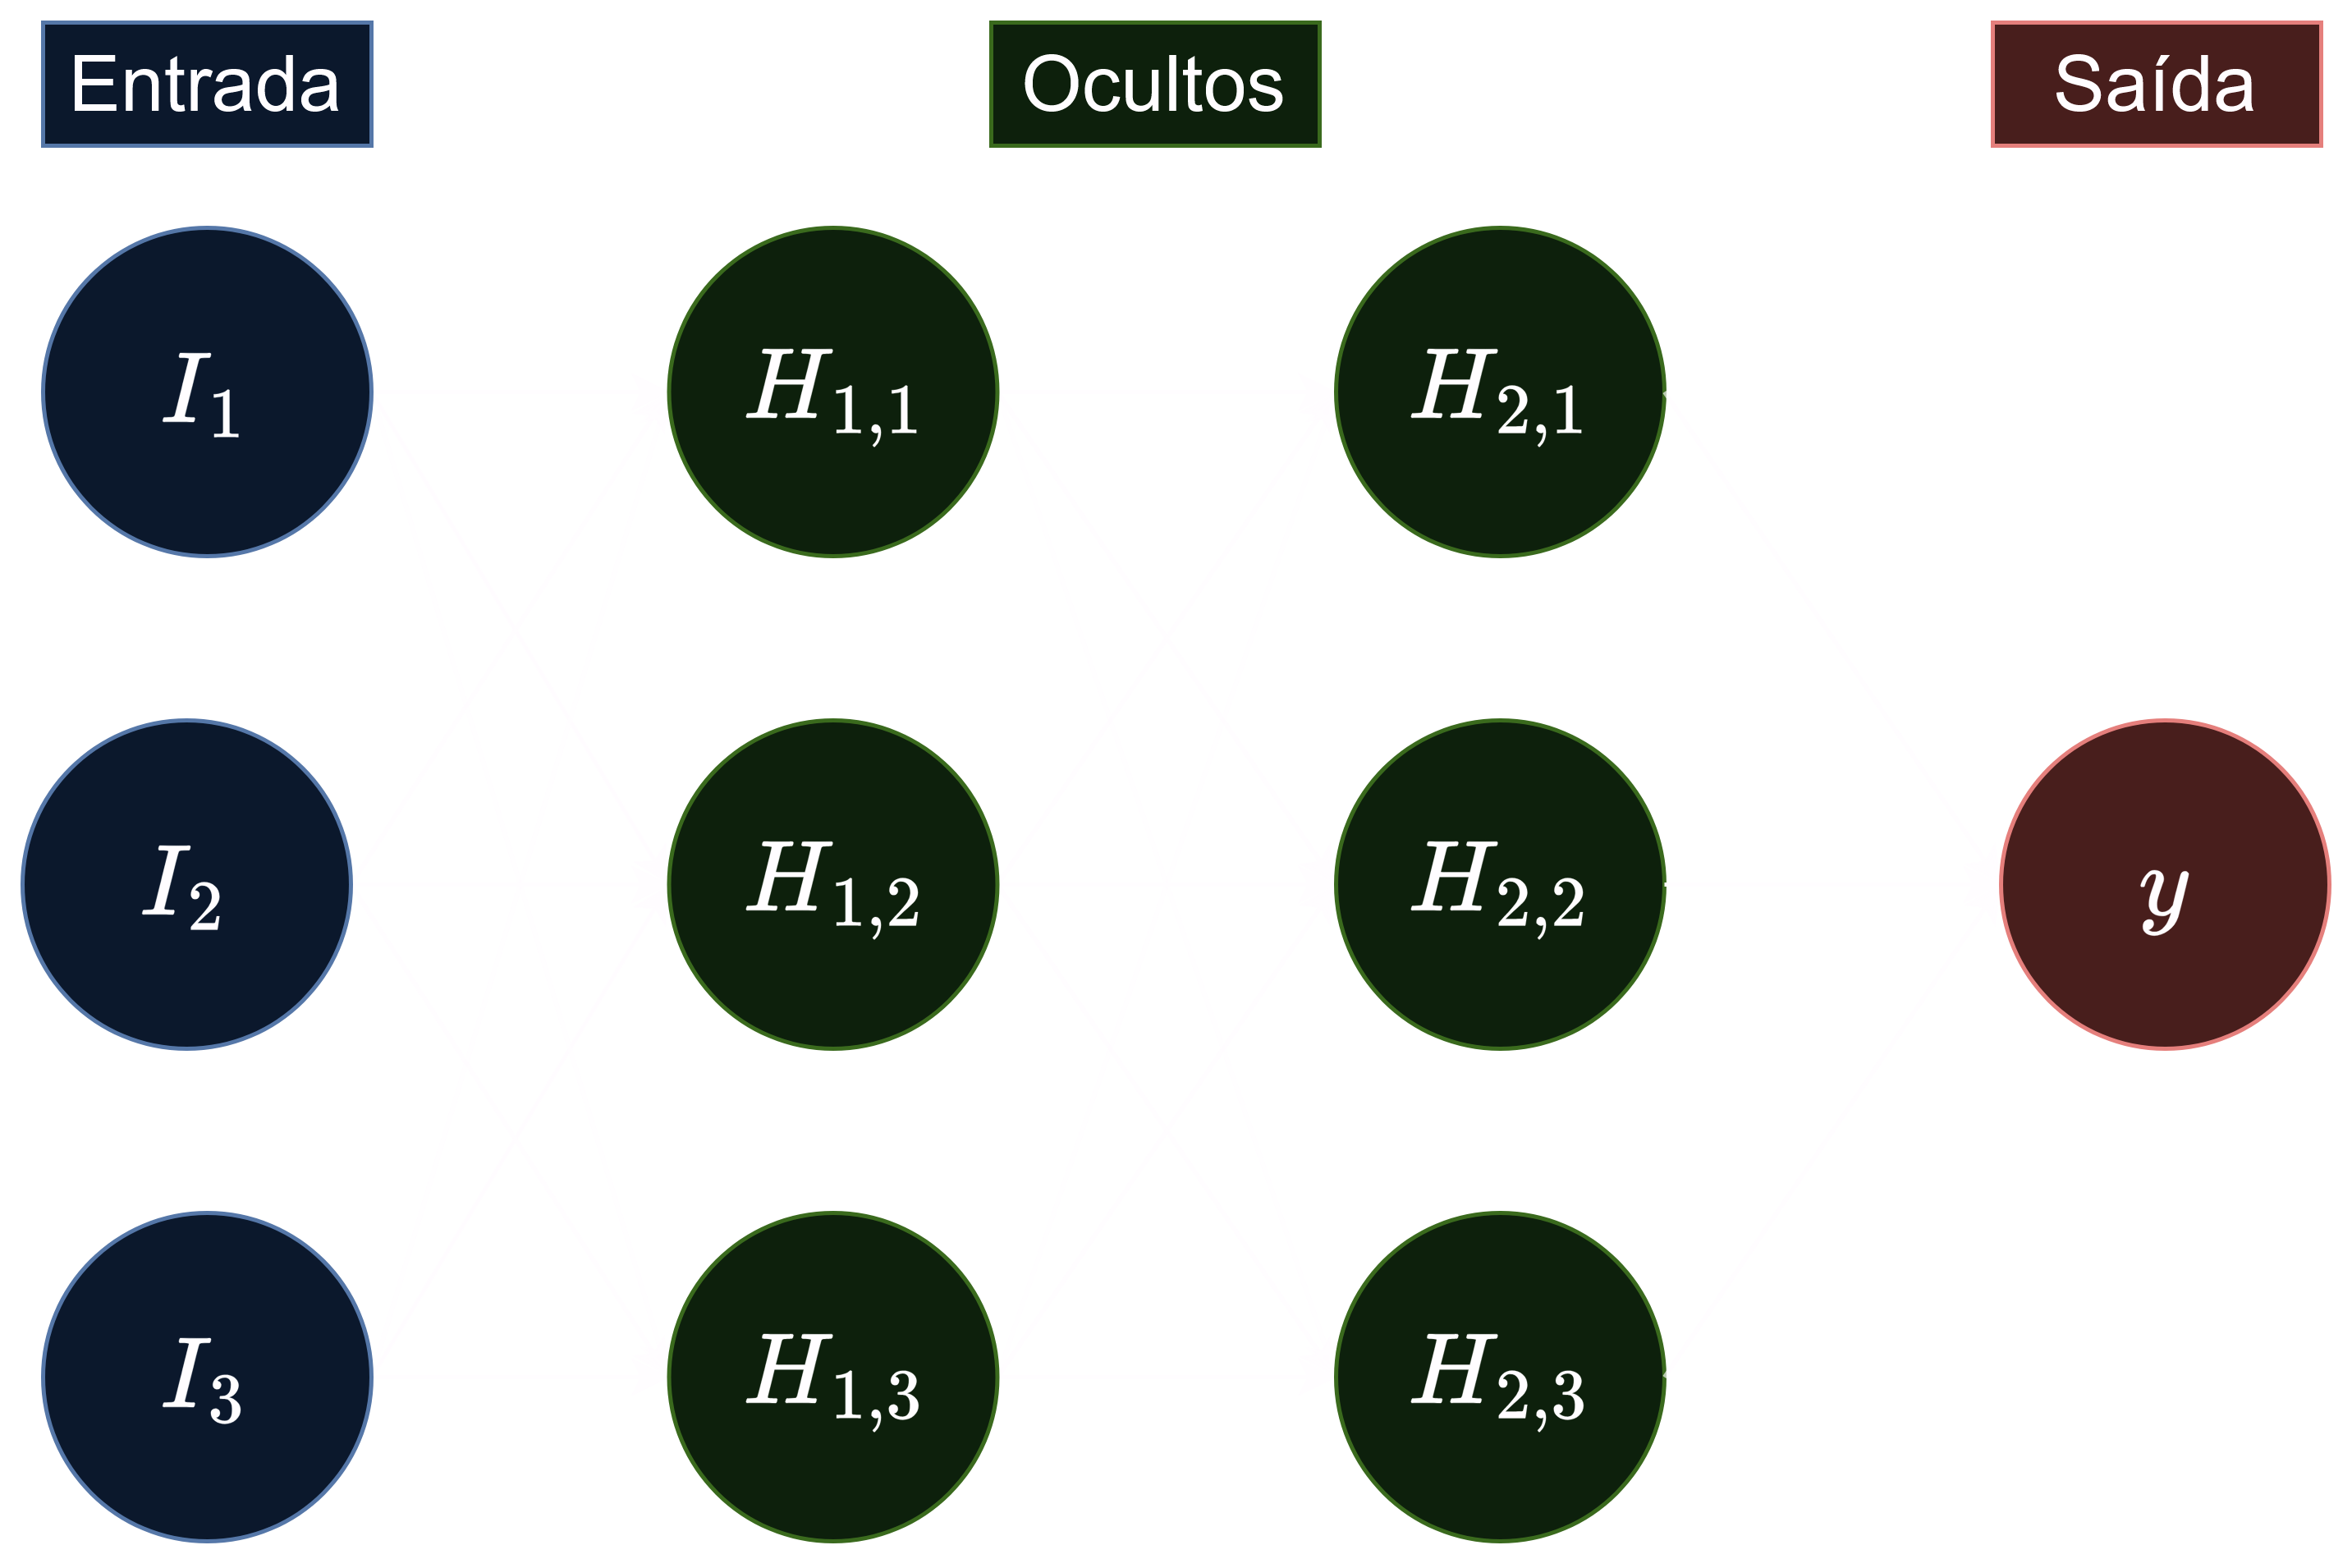
\includegraphics[height=6cm]{script/images/rede_normal.png}
% %     \end{figure}
% % \end{frame}

% \begin{frame}[c]{Redes neurais Bayesianas}
%     \begin{figure}
%         \centering
%         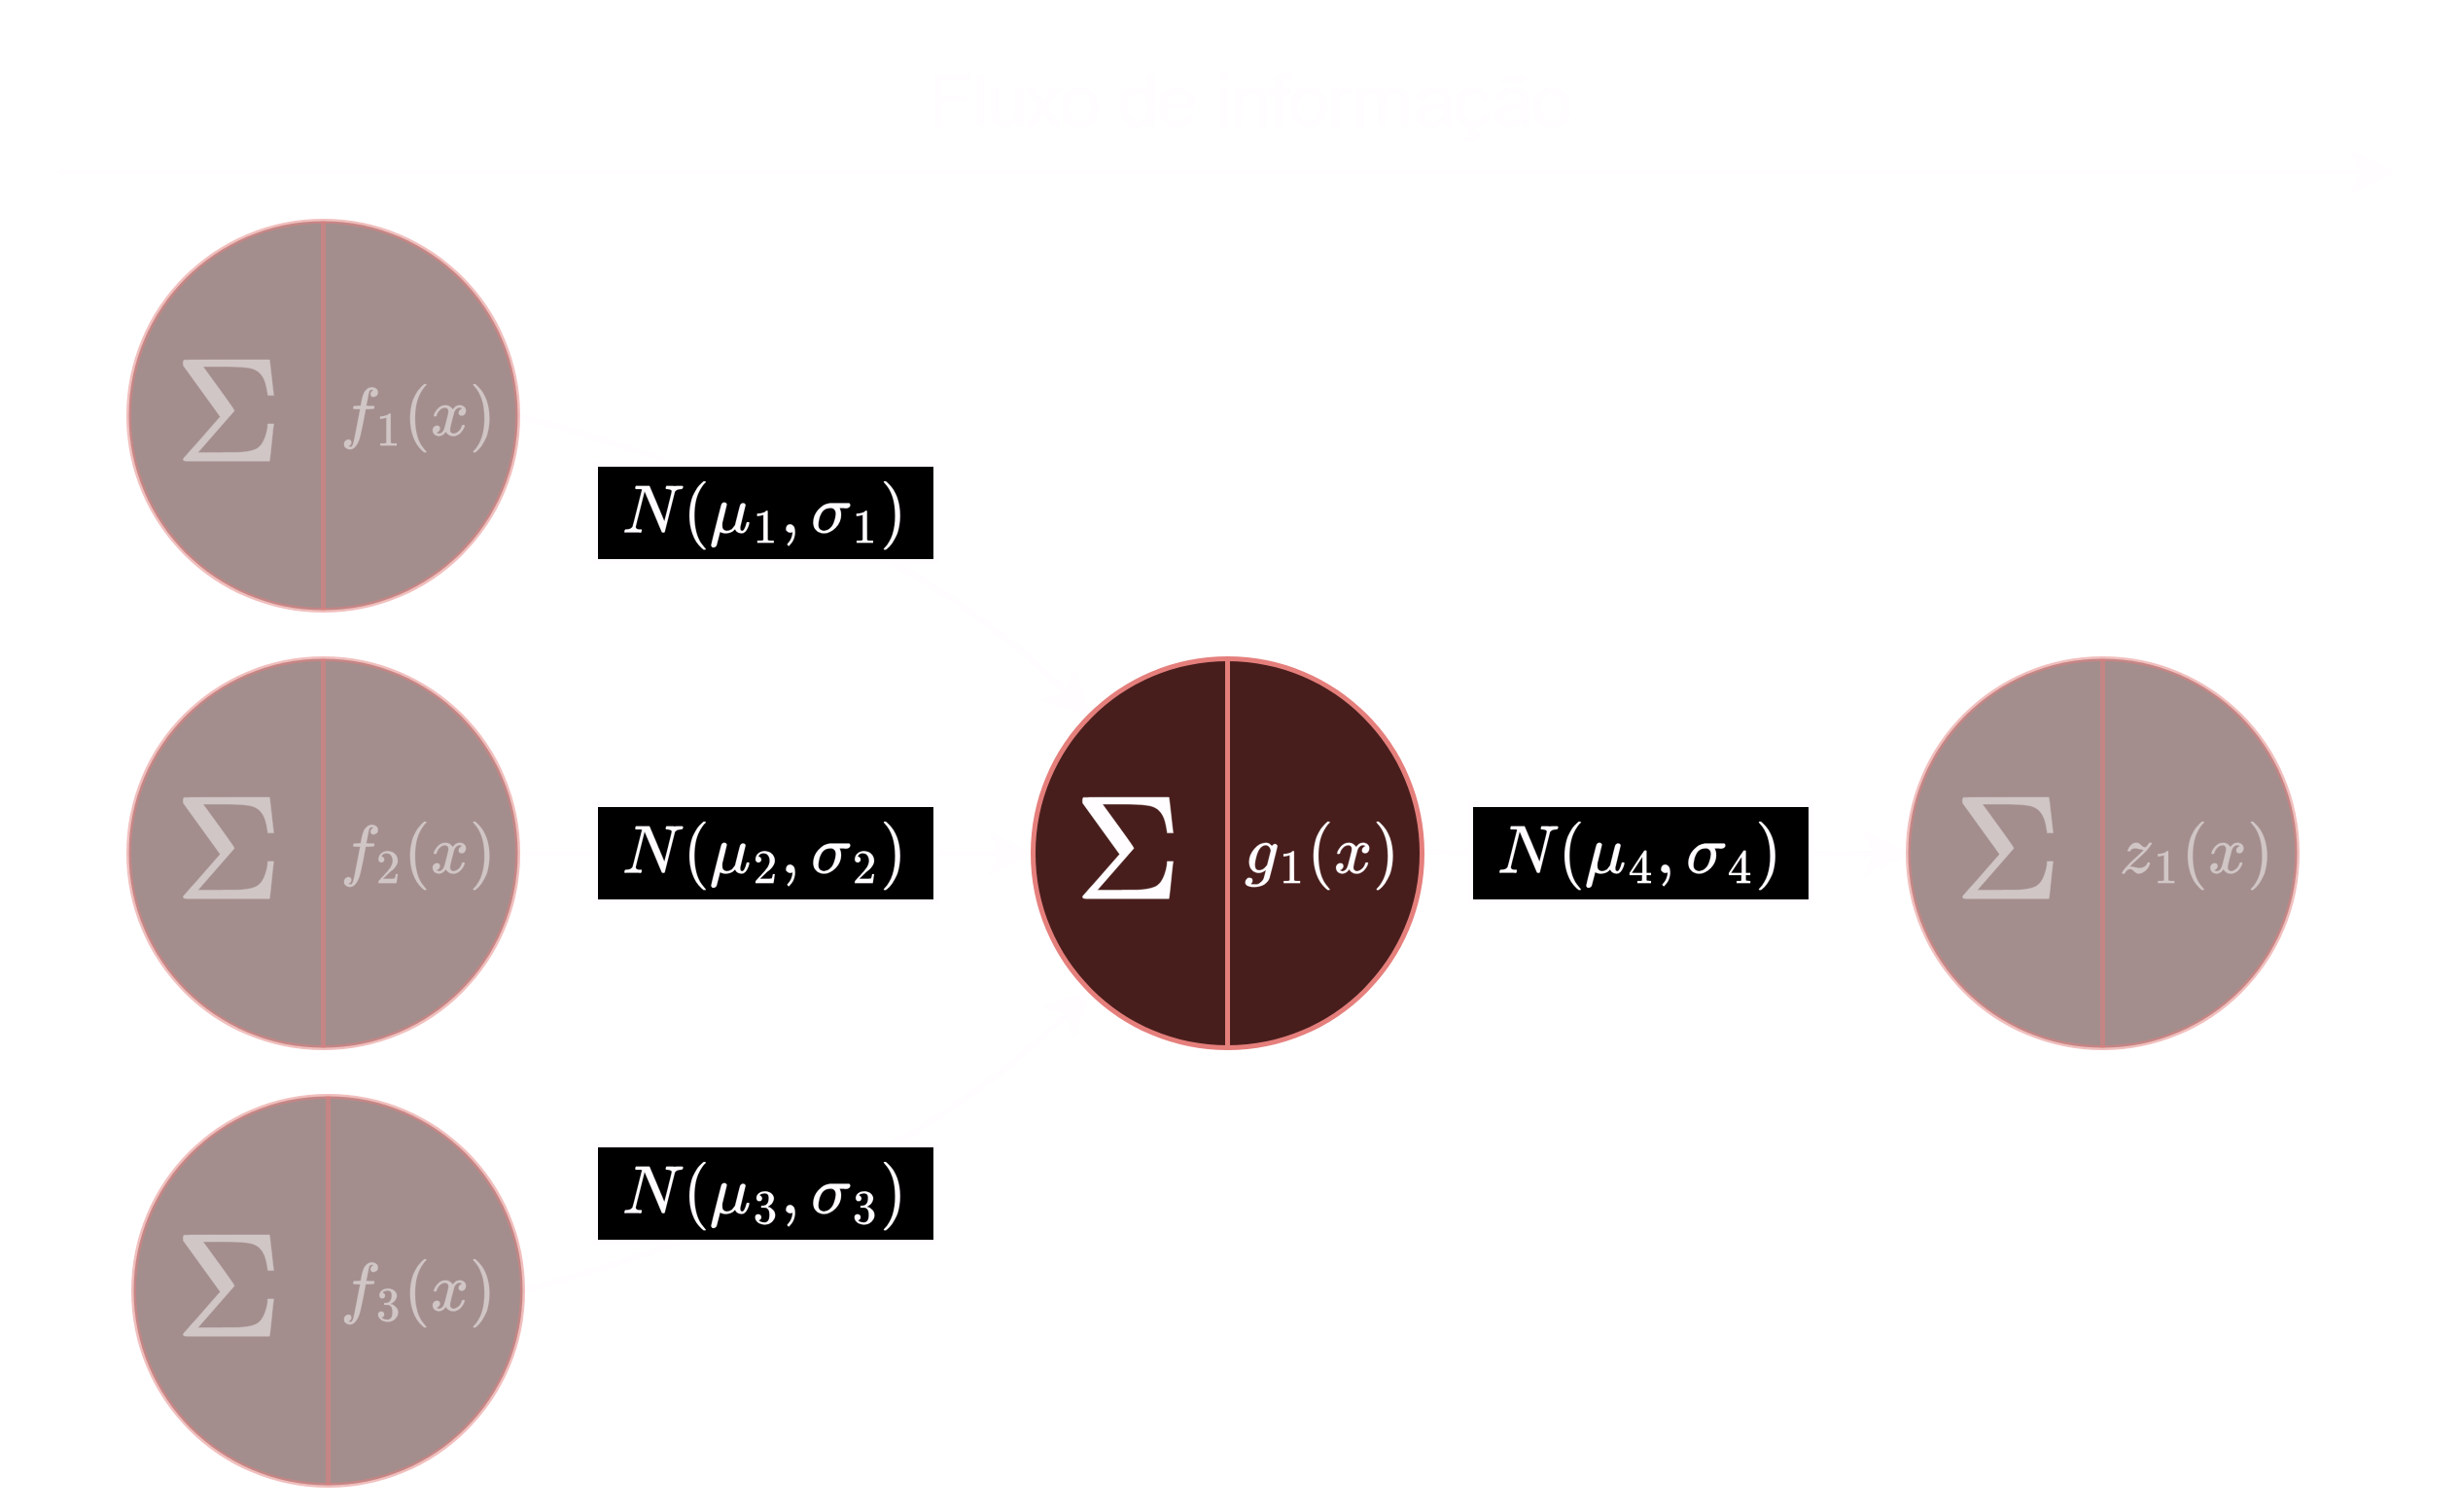
\includegraphics[height=6cm]{script/images/neuron_ml_bayes.png}
%     \end{figure}
% \end{frame}

% \begin{frame}[c]{Redes de mistura de densidades}
%     \begin{figure}
%         \centering
%         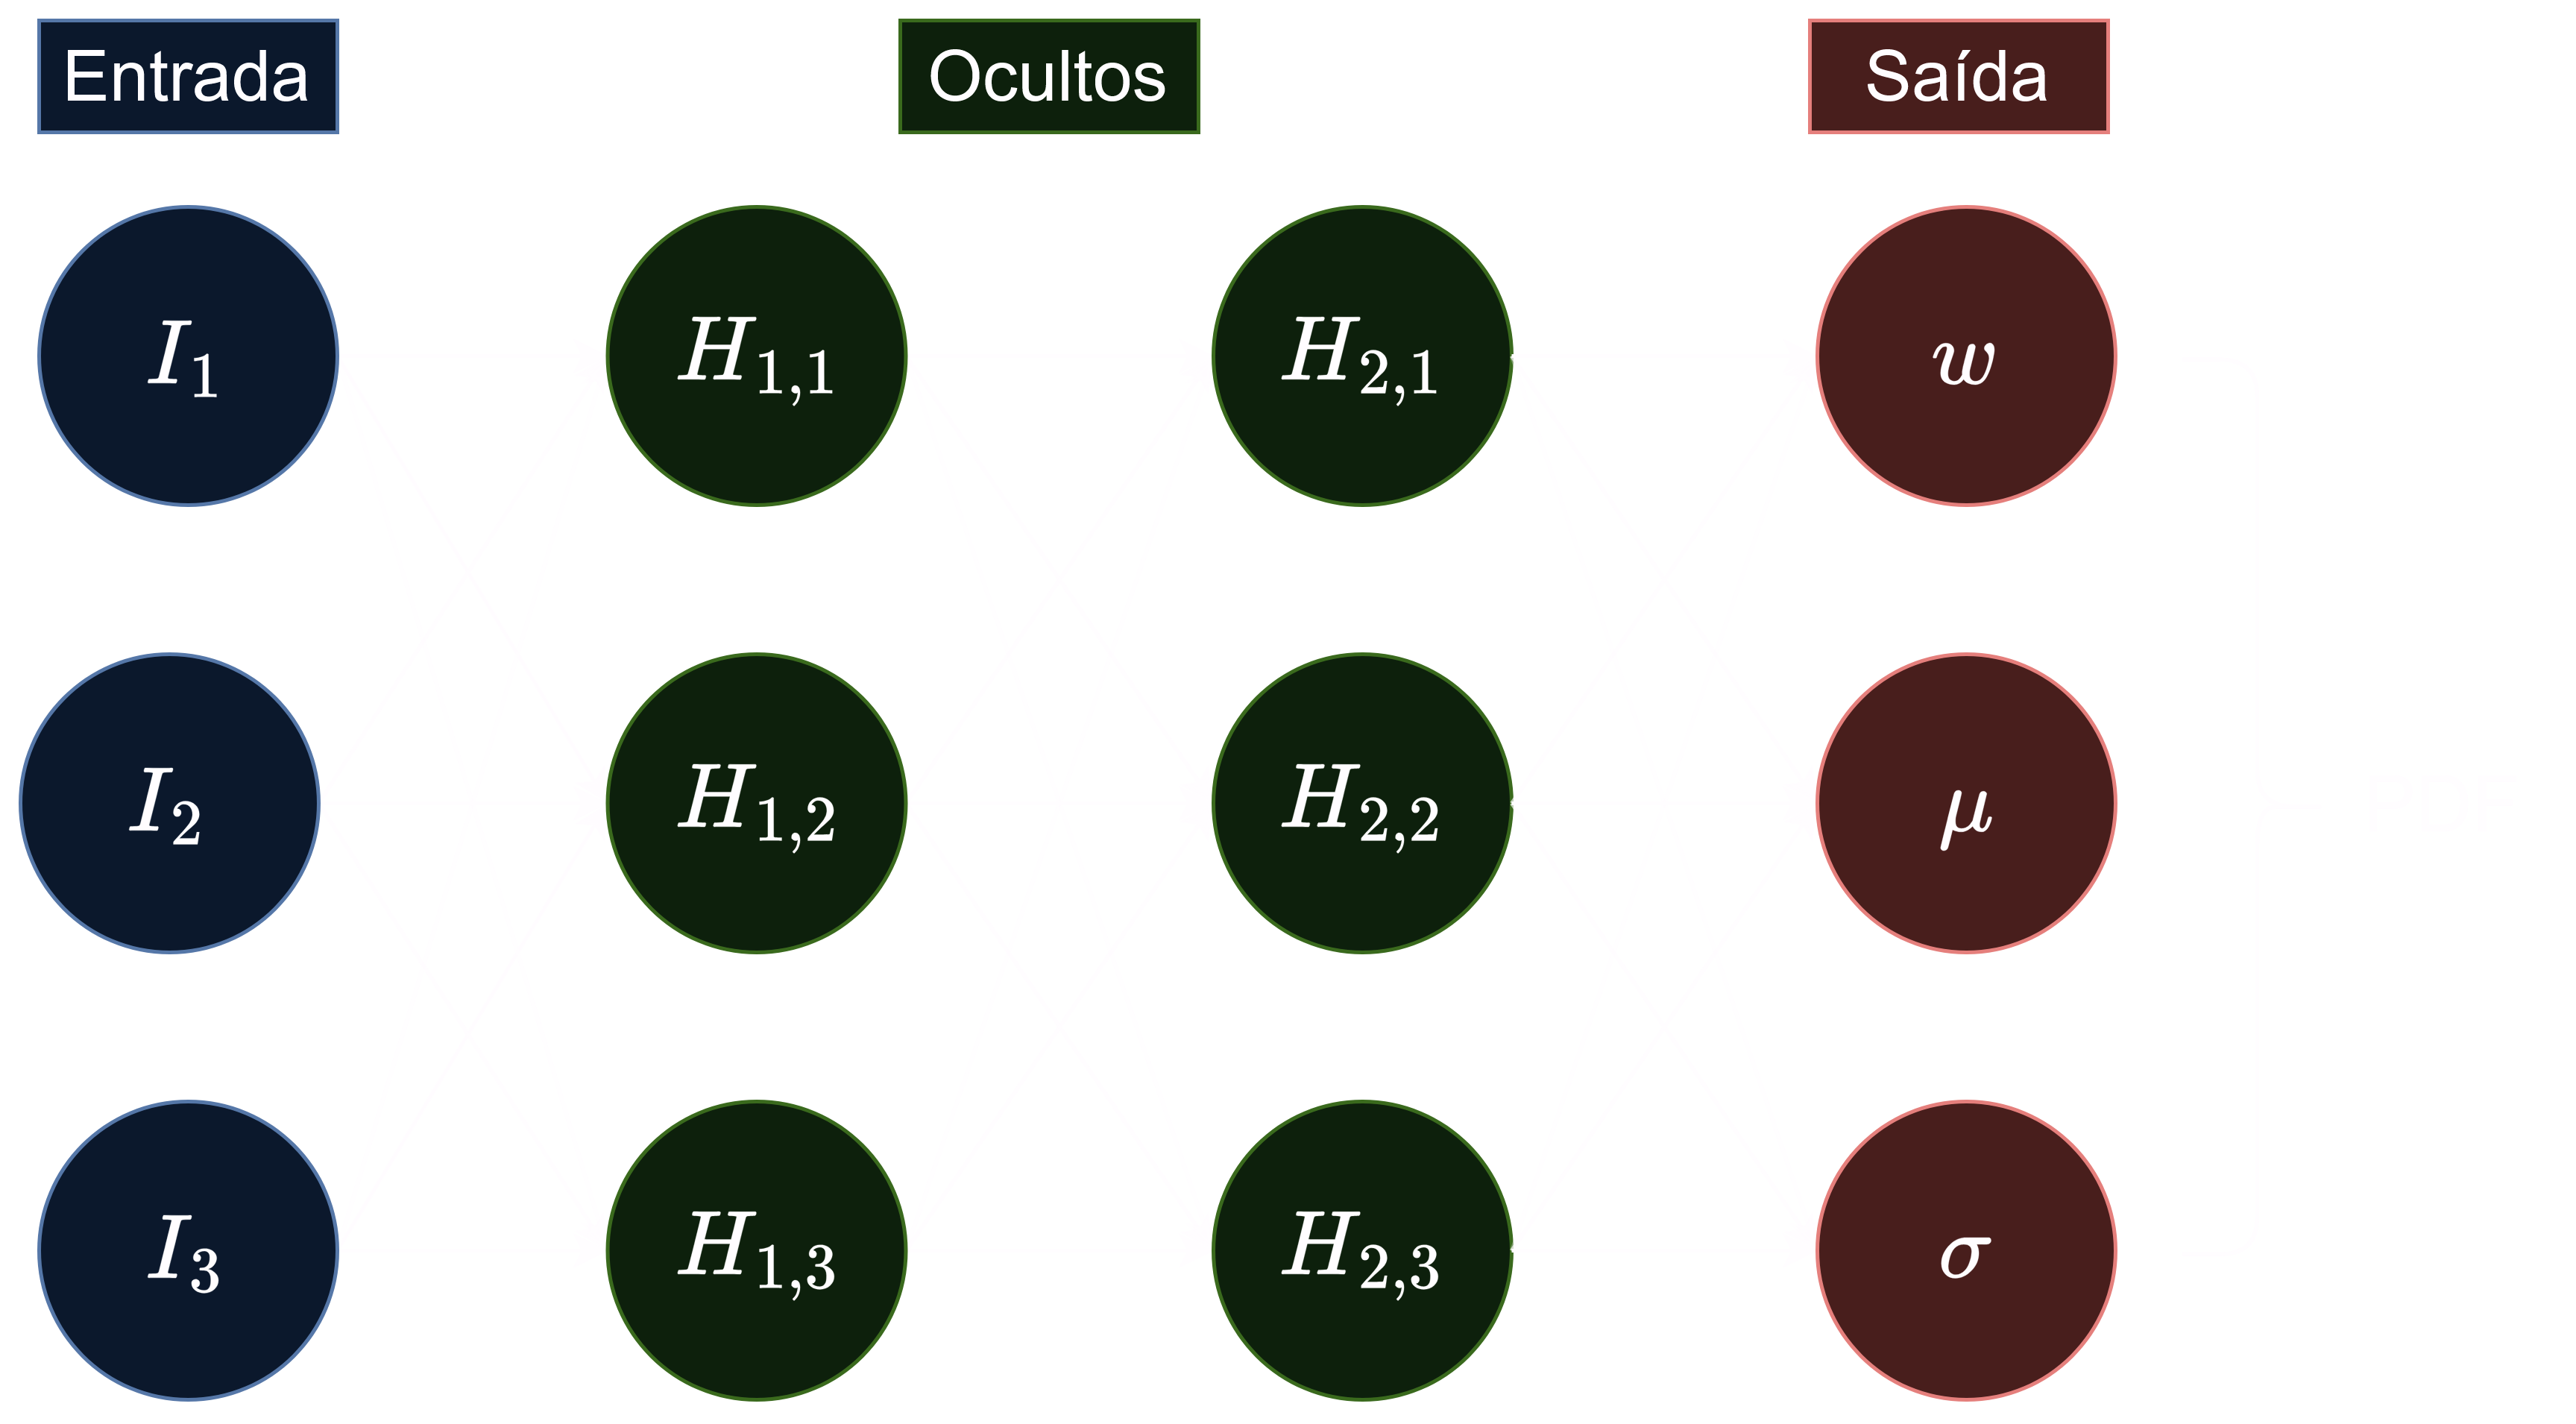
\includegraphics[height=6cm]{script/images/rede_mdn.png}
%     \end{figure}
% \end{frame}

% \begin{frame}[c]{Redes de mistura de densidades}
%     \begin{figure}
%         \centering
%         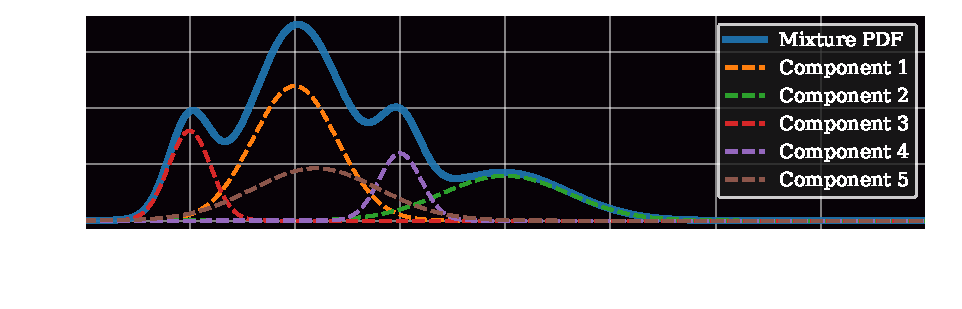
\includegraphics[width=\linewidth]{script/images/mixture_pdf_5comp.pdf}
%     \end{figure}
% \end{frame}

% \begin{frame}[c]{Redes de mistura de densidades Bayesiana}
%     Usamos uma combinação da abordagem Bayesiana com a de mistura de densidades, criando uma rede cujos pesos são distribuições e que, como saida, fornece $N$ componentes de uma mistura de densidades.

%     \begin{columns}[c]
%         \begin{column}{0.46\textwidth}
%             \begin{splusbox}{Bayesian Neural Network}
%                 \begin{itemize}
%                     \item Modelagem de incertezas
%                     \begin{itemize}
%                         \item Aleatória (dos dados)
%                         \item Epistêmica (do modelo)
%                     \end{itemize}
%                 \end{itemize}
%             \end{splusbox}
%         \end{column}
%         \begin{column}{0.46\textwidth}
%             \begin{splusbox}{Mixture Density Network}
%                 \begin{itemize}
%                     \item Gera PDFs bem calibradas diretamente, inteiramente descritas por poucos parâmetros
%                     \item É eficiente em termos de armazenamento
%                 \end{itemize}
%             \end{splusbox}
%         \end{column}
%     \end{columns}

%     % \begin{itemize}
%     %     \justifying
%     %     \item A abordagem Bayesiana permite que a rede leve em conta incertezas inerentes do problema, como aquelas devido à medição da fotometria (aleatória) e das estimativas do modelo (epistêmica).
%     %     \item É capaz de produzir funções de densidade de probabilidade (PDFs) de forma natural e direta, sendo que estas são calibradas durante o treinamento do modelo.
%     % \end{itemize}
% \end{frame}

% \section{Definindo a arquitetura}
% \begin{frame}[c]{Definindo a arquitetura da rede com o \texttt{Optuna}}
%     \begin{figure}
%         \centering
%         \includegraphics[width=\linewidth]{script/images/optuna_metrics_scatter.pdf}
%     \end{figure}
% \end{frame}

% % \begin{frame}[c]{Definindo a arquitetura da rede com o \texttt{Optuna}}
% %     \begin{columns}[c]
% %         \small
% %         \begin{column}{0.49\textwidth}
% %             \begin{splusbox}{Parâmetros para amostrar}
% %                 Para cada abertura do SPLUS:
% %                 \begin{itemize}
% %                     \item Camadas: 3 a 6
% %                     \item Neurônios por camada: 64 a 128
% %                     \item Função de ativação: leakyrelu, relu, elu, gelu, selu, prelu, rrelu, silu, mish, celu
% %                     \item Viés nas camadas: Verdadeiro ou Falso
% %                     \item Camada de atenção por feature: Verdadeiro ou falso
% %                     \item Learning rate: 0.001 a 0.03
% %                     \item Weight decay: 0.000001 a 0.0001
% %                     \item Otimizador: adam, nadam, adamw, adabelief, ranger
% %                 \end{itemize}
% %             \end{splusbox}
% %         \end{column}
% %         \begin{column}{0.49\textwidth}
% %             \begin{splusbox}{Parâmetros escolhidos}
% %                 Abertura PStotal
% %                 \begin{itemize}
% %                     \item Camadas: 4
% %                     \item Neurônios: 64
% %                     \item Função de ativação: gelu
% %                     \item Viés nas camadas: Verdadeiro
% %                     \item Camada de atenção por feature: Verdadeiro
% %                     \item Learning rate: 0.0296
% %                     \item Weight decay: $7.5 \times 10^{-6}$
% %                     \item Otimizador: adabelief
% %                 \end{itemize}
% %             \end{splusbox}
% %         \end{column}
% %     \end{columns}
% % \end{frame}

% \begin{frame}[c]{Definindo a arquitetura da rede com o \texttt{Optuna}}
%     \begin{table}
%         \centering
%           \begin{tabular}{@{}lll@{}}
%               \toprule
%               \textbf{Variável}   & \textbf{Parâmetros para amostrar}     & \textbf{Parâmetros escolhidos} \\ \midrule
%               Camadas             & 3 a 6                                 & 4                              \\
%               Neurônios           & 64 a 128                              & 64                             \\
%               Ativação            & Todas as "\texttt{LU}"                  & \texttt{gelu}                  \\
%               Otimizador          & Variações de \texttt{Adam}            & \texttt{AdaBelief}             \\
%               Learning rate       & 0.001 a 0.03                          & 0.0296                         \\
%               Weight decay        & $1 \times 10^{-6}$ a $1 \times 10^{-4}$ & $7.5 \times 10^{-6}$           \\
%               Viés das camadas    & \texttt{True} ou \texttt{False}       & \texttt{True}                  \\
%               Atenção por feature & \texttt{True} ou \texttt{False}       & \texttt{True}                  \\ \bottomrule
%           \end{tabular}
%       \end{table}

%       \begin{tcolorbox}
%           Em todos os casos, os valores de entrada foram   magnitudes, cores e informações morfológicas
%       \end{tcolorbox}
% \end{frame}

% \section{Resultados}
% % \begin{frame}[c]{Redshifts fotométricos: estimativas de ponto único}
% %     \begin{itemize}
% %         \item $\sigma_\text{NMAD}$:
% %         \begin{equation*}
% %             \sigma_\text{NMAD} = 1.48 \times \text{mediana} \left( \left| \frac{{\delta z} - \text{mediana}(\delta z)}{1+z_\text{spec}} \right| \right)
% %         \end{equation*}
% %         \item Bias ($\mu$):
% %         \begin{align*}
% %             \mu &= \text{mediana} \left( \delta z \right), \\
% %             \mu_\text{norm} &= \text{mediana} \left( \frac{\delta z}{1+z_{\text{spec}}} \right).
% %         \end{align*}
% %         \item Fração de outliers ($\eta$):
% %         \begin{align*}
% %             \eta &= \frac{|\delta z|}{1+z_\text{spec}} > 0.15, \\
% %             \eta_{N\sigma} &= \frac{|\delta z|}{1+z_\text{spec}} > N \cdot \sigma_\text{NMAD}.
% %         \end{align*}
% %     \end{itemize}
% % \end{frame}

% \begin{frame}[c]{Redshifts fotométricos: estimativas de ponto único}
%     \begin{splusbox}{Desvio médio absoluto normalizado ($\sigma_\text{NMAD}${, \textcolor{LightGray}{Brammer et al., 2008}})}
%         \begin{equation*}
%             \sigma_\text{NMAD} = 1.48 \times \text{mediana} \left( \left| \frac{{\delta z} - \text{mediana}(\delta z)}{1+z_\text{spec}} \right| \right)
%         \end{equation*}
%     \end{splusbox}

%     % \begin{splusbox}{Desvio médio absoluto normalizado ($\sigma_\text{NMAD}$)}
%     %     \vspace{-.5cm}
%     %     \begin{columns}[c]
%     %         \begin{column}{0.58\textwidth}
%     %             \centering
%     %             \begin{equation*}
%     %                 \sigma_\text{NMAD} = 1.48 \times \text{mediana} \left( \left| \frac{{\delta z} - \text{mediana}(\delta z)}{1+z_\text{spec}} \right| \right)
%     %             \end{equation*}
%     %         \end{column}
%     %         \begin{column}{0.38\textwidth}
%     %             \centering
%     %             \begin{equation*}
%     %                 \delta z = z_\text{phot} - z_\text{spec}
%     %             \end{equation*}
%     %         \end{column}
%     %     \end{columns}
%     % \end{splusbox}

%     \begin{splusbox}{Viés ($\mu$)}
%         \vspace{-.5cm}
%         \begin{columns}[c]
%             \begin{column}{0.46\textwidth}
%                 \centering
%                 \begin{equation*}
%                     \mu = \text{mediana} \left( \delta z \right)
%                 \end{equation*}
%             \end{column}
%             \begin{column}{0.46\textwidth}
%                 \centering
%                 \begin{equation*}
%                     \mu_\text{norm} = \text{mediana} \left( \frac{\delta z}{1+z_{\text{spec}}} \right)
%                 \end{equation*}
%             \end{column}
%             \hspace*{1cm}
%         \end{columns}
%     \end{splusbox}

%     \begin{splusbox}{Fração de outliers ($\eta${, {\textcolor{LightGray}{Ilbert et al., 2006; Dahlen et al., 2013}}})}
%         \vspace{-.5cm}
%         \begin{columns}[c]
%             \begin{column}{0.46\textwidth}
%                 \centering
%                 \begin{equation*}
%                     \eta = \frac{|\delta z|}{1+z_\text{spec}} > 0.15
%                 \end{equation*}
%             \end{column}
%             \begin{column}{0.46\textwidth}
%                 \centering
%                 \begin{equation*}
%                     \eta_{N\sigma} = \frac{|\delta z|}{1+z_\text{spec}} > N \cdot \sigma_\text{NMAD}
%                 \end{equation*}
%             \end{column}
%             \hspace*{1cm}
%         \end{columns}
%     \end{splusbox}
% \end{frame}

% \begin{frame}[c]{Redshifts fotométricos: estimativas de ponto único}
%     \begin{figure}
%         \centering
%         \includegraphics[height=7cm]{script/images/results_scatterplot_residuals.pdf}
%     \end{figure}
% \end{frame}

% \begin{frame}[c]{Redshifts fotométricos: estimativas de ponto único}
%     \begin{figure}
%         \centering
%         \includegraphics[height=7cm]{script/images/results_spe_metrics.pdf}
%     \end{figure}
% \end{frame}

% \begin{frame}[c]{Redshifts fotométricos: estimativas de ponto único}
%     \begin{figure}
%         \centering
%         \includegraphics[width=\linewidth]{script/images/results_spe_metrics_2d.pdf}
%     \end{figure}
% \end{frame}

% \begin{frame}[c]{Redshifts fotométricos: estimativas de ponto único}
%     Para verificar se a distribuição de photo-zs está como é esperado, comparamos os resultados que obtemos com os resultados de dois outros modelos, um KNN e uma RF, para objetos na Stripe-82.

%     \begin{figure}
%         \centering
%         \includegraphics[width=0.8\linewidth]{script/images/s82_redshifts.pdf}
%     \end{figure}
% \end{frame}

% \begin{frame}[c]{Redshifts fotométricos: funções de densidade de probabilidade}
%     % \begin{itemize}
%     %     \item Odds \textcolor{LightGray}{(Benitez, 2000)}
%     %     \item Highest Probability Density Credible Interval \textcolor{LightGray}{(Wittman et al., 2016)}
%     %     \item Probability Integral Transform \textcolor{LightGray}{(Polsterer et al., 2016)}
%     %     %\item Continuous Ranked Probability Score \textcolor{LightGray}{(Hersbach, 2000; Polsterer et al., 2016)}
%     %     \item $\sigma_{68}$ e valor máximo
%     % \end{itemize}

%     \begin{splusbox}{Odds \textcolor{LightGray}{(Benitez, 2000)}}
%         \small
%         \vspace{-.5cm}
%         \begin{align*}
%           \text{odds}_i = \int_{z_\text{peak, $i$}-\Delta z}^{z_\text{peak, $i$}+\Delta z} \text{PDF}_i(z)~\text{d}z,
%         \end{align*}
%     \end{splusbox}

%     \begin{splusbox}{Probability Integral Transform \textcolor{LightGray}{(Polsterer et al., 2016)}}
%         \small
%         \vspace{-.5cm}
%         \begin{align*}
%             \text{PIT}_i = \int_{0}^{z_\text{spec}} \text{PDF}_i(z)~\text{d}z = \text{CDF}_i(z_\text{spec}).
%           \end{align*}
%     \end{splusbox}

%     \centering
%     \begin{tcolorbox}[hbox]
%         \small
%         Highest Probability Density Credible Interval \textcolor{LightGray}{(Wittman et al., 2016)}
%     \end{tcolorbox}

%     \begin{tcolorbox}[hbox]
%         \small
%         $\sigma_{68}$ e valor máximo
%     \end{tcolorbox}

% \end{frame}

% \begin{frame}[c]{Redshifts fotométricos: funções de densidade de probabilidade}
%     \begin{figure}
%         \centering
%         \includegraphics[height=7cm]{script/images/results_pdf_metrics_illust_2.pdf}
%     \end{figure}
% \end{frame}

% % \begin{frame}[c]{Redshifts fotométricos: funções de densidade de probabilidade}
% %     PDF: apresentar métricas, histogramas de calibração, resultados por campo
% % \end{frame}

% \begin{frame}[c]{Redshifts fotométricos: funções de densidade de probabilidade}
%     \begin{figure}
%         \centering
%         \includegraphics[height=7cm]{script/images/result_pdf_summary.pdf}
%     \end{figure}
% \end{frame}

% \begin{frame}[c]{Redshifts fotométricos: funções de densidade de probabilidade}
%     \begin{figure}
%         \centering
%         \includegraphics[width=\linewidth]{script/images/results_pdf_metrics_2d.pdf}
%     \end{figure}
% \end{frame}

% \section{Estrutura em larga escala}
% \begin{frame}[c]{Estrutura em larga escala}
%     \begin{figure}
%         \centering
%         \includegraphics[width=\linewidth]{script/images/lss_problem.pdf}
%     \end{figure}
%     %
%     \centering
%     \begin{tcolorbox}[hbox] % <---
%         Interpretamos que o $z_\text{phot}$ é igual a $z_\text{spec} + \epsilon$
%     \end{tcolorbox}
%     % \begin{splusbox}{}
%     %     \centering
%     %     Interpretamos que o $z_\text{phot}$ é igual a $z_\text{spec} + \epsilon$
%     % \end{splusbox}
% \end{frame}

% % \begin{frame}[c]{Estrutura em larga escala}
% %     \begin{splusbox}{Autoencoders e U-Nets}
% %         Redes desenvolvidas especificamente para fazer compressão de dados, podendo remover ruído
% %     \end{splusbox}

% %     \begin{splusbox}{Denoising Diffusion Probabilistic Models (DDPMs)}
% %         Redes que utilizam um processo de difusão (e difusão inversa) para aprender uma distribuição que representa os dados, podem ser utilizadas para remover ruído
% %     \end{splusbox}

% %     \begin{splusbox}{Graph Neural Networks (GNNs)}
% %         Redes que utilizam outra estrutura de dados (grafos), e que é capaz de utilizar informação de posição e relação entre amostras para melhorar seus resultados
% %     \end{splusbox}
% % \end{frame}

% \begin{frame}[c]{Estrutura em larga escala}
%     \centering
%     % \begin{splusbox}{}
%     %     \large Autoencoders e U-Nets
%     % \end{splusbox}

%     % \begin{splusbox}{}
%     %     \large Denoising Diffusion Probabilistic Models (DDPMs)
%     % \end{splusbox}

%     % \begin{splusbox}{}
%     %     \large Graph Neural Networks (GNNs)
%     % \end{splusbox}

%     \begin{tcolorbox}[hbox] % <---
%         \large Autoencoders e U-Nets
%     \end{tcolorbox}
%     \vspace{0.5cm}
%     \begin{tcolorbox}[hbox] % <---
%         \large Denoising Diffusion Probabilistic Models (DDPMs)
%     \end{tcolorbox}
%     \vspace{0.5cm}
%     \begin{tcolorbox}[hbox] % <---
%         \large Graph Neural Networks (GNNs)
%     \end{tcolorbox}
% \end{frame}

% \begin{frame}[c]{Autoencoders {\small \textcolor{LightGray}{(Kramer, 1991; Kingma e Welling, 2013; Ronnerberger et al., 2015)}}}
%     \begin{columns}[c]
%         \begin{column}{0.36\linewidth}
%             \begin{splusbox}{}
%                 \begin{itemize}
%                     \justifying
%                     \item São caracterizadas pela existência de um gargalo
%                     \item Treinamento simultâneo de duas redes
%                     \item Tem como objetivo reproduzir o input com menos informação
%                     \item Remove ruído pois ele não é fundamental na reconstrução do input
%                 \end{itemize}
%             \end{splusbox}
%         \end{column}
%         \begin{column}{0.56\linewidth}
%             \begin{figure}
%                 \centering
%                 \includegraphics[height=6.5cm]{script/images/autoencoders.png}
%             \end{figure}
%         \end{column}
%     \end{columns}
% \end{frame}

% \begin{frame}[c]{Autoencoders}
%     \begin{figure}
%         \centering
%         \includegraphics[width=\linewidth]{script/images/redshift_polar_plot_zml_zmlae_zmlvae.pdf}
%     \end{figure}
% \end{frame}

% \begin{frame}[c]{Autoencoders}
%     \begin{figure}
%         \centering
%         \includegraphics[height=7cm]{script/images/2pcf_compare_corrfunc.pdf}
%     \end{figure}
% \end{frame}

% \begin{frame}[c]{Denoising Diffusion Probabilistic Models  {\small \textcolor{LightGray}{(Ho et al., 2020)}}}
%     \begin{figure}
%         \centering
%         \includegraphics[width=\linewidth]{script/images/diffusion.png}
%         \caption{Adaptado de \url{https://cvpr2022-tutorial-diffusion-models.github.io/}.}
%     \end{figure}

%     \centering
%     \begin{splusbox}{}
%         É capaz de modelar as incertezas sem suposições simples (por ex. erros são Gaussianos), e pode aprender correlações nas incertezas do photo-z
%     \end{splusbox}
%     % \begin{tcolorbox}[hbox]
%     %     É capaz de modelar as incertezas sem suposições simples (por ex. erros são Gaussianos), e pode aprender correlações nas incertezas do photo-z
%     % \end{tcolorbox}
% \end{frame}

% % \begin{frame}[c]{Denoising Diffusion Probabilistic Models}
% %     \begin{splusbox}{}
% %         \begin{itemize}
% %             \item Modelagem das incertezas como um forward-process
% %             \item É capaz de aprender correlações e efeitos não-Gaussianos nas incertezas do photo-z
% %             %\item Condicionamento na fotometria, permitindo a obtenção de um photo-z mais próximo ao spec-z diretamente, contornando a necessidade de passos intermediários
% %             \item Fornece estimativas probabilísticas
% %         \end{itemize}
% %     \end{splusbox}
% % \end{frame}

% \begin{frame}[c]{Denoising Diffusion Probabilistic Models}
%     \begin{columns}[c]
%         \begin{column}{0.46\linewidth}
%             \begin{splusbox}{Tabular}
%                 \begin{itemize}
%                     \item[$\checkmark$] Lida com a estrutura natural dos dados
%                     \item[$\checkmark$] Computacionalmente mais leve
%                     \item[$\times$] Sem possibilidade de aprender relações espaciais
%                     \item[$\times$] Não usa arquiteturas comuns a esse problema
%                 \end{itemize}
%             \end{splusbox}
%         \end{column}
%         \begin{column}{0.46\linewidth}
%             \begin{splusbox}{Imagens}
%                 \begin{itemize}
%                     \item[$\checkmark$] Usa arquiteturas conhecidas (U-Net)
%                     \item[$\checkmark$] Aprenderia relações espaciais
%                     \item[$\checkmark$] Entendimento mais simples
%                     \item[$\times$] Computacionalmente mais pesado
%                     \item[$\times$] Modifica a forma natural dos dados
%                 \end{itemize}
%             \end{splusbox}
%         \end{column}
%     \end{columns}
% \end{frame}

% \begin{frame}[c]{Denoising Diffusion Probabilistic Models}
%     \begin{figure}
%         \centering
%         \includegraphics[width=\linewidth]{script/images/lss_illustration.pdf}
%     \end{figure}
%     %
%     \begin{splusbox}{}
%         \begin{itemize}
%             \item O ruído é modelado de forma que partimos de $z_\text{spec}$ e chegamos em $z_\text{phot}$
%             \item O modelo é condicionado na fotometria, dispensando a necessidade de saber o timestep $t$
%         \end{itemize}
%     \end{splusbox}
% \end{frame}

% \begin{frame}[c]{Denoising Diffusion Probabilistic Models}
%     \begin{figure}
%         \centering
%         \includegraphics[height=7cm]{script/images/ddpm_diffusion_features.pdf}
%     \end{figure}
% \end{frame}

% \begin{frame}[c]{Denoising Diffusion Probabilistic Models}
%     \begin{figure}
%         \centering
%         \includegraphics[height=7cm]{script/images/ddpm_diffusion_z.pdf}
%     \end{figure}
% \end{frame}

% \begin{frame}[c]{Graph Neural Networks {\small \textcolor{LightGray}{(Gori et al., 2005; Scarselli et al., 2009)}}}
%     \begin{columns}[c]
%         \begin{column}{0.46\linewidth}
%             \begin{splusbox}{}
%                 \begin{itemize}
%                     \justifying
%                     \item Sistemas de recomendação
%                     \item Detecção de fraudes
%                     \item Descoberta de medicamentos
%                     \item Identificação de estruturas de proteínas
%                     \item Otimização de cadeias de produção
%                 \end{itemize}
%             \end{splusbox}
%         \end{column}
%         \begin{column}{0.46\linewidth}
%             \begin{figure}
%                 \centering
%                 \includegraphics[height=5.5cm]{images/planetoidcora.png}
%                 \caption{Adaptado de \url{https://graphsandnetworks.com/the-cora-dataset/}}
%             \end{figure}
%         \end{column}
%     \end{columns}
% \end{frame}

% \begin{frame}[c]{Graph Neural Networks}
%     \begin{figure}
%         \centering
%         \includegraphics[height=7cm]{images/galaxy_graph.pdf}
%     \end{figure}
% \end{frame}

% \begin{frame}[c]{Graph Neural Networks}
%     \begin{figure}
%         \centering
%         \includegraphics[height=7cm]{images/galaxy_graph_gnn.pdf}
%     \end{figure}
% \end{frame}

% \begin{frame}[c]{Graph Neural Networks}
%     \begin{figure}
%         \centering
%         \includegraphics[width=0.9\linewidth]{images/gnn_message.png}
%         \caption{Adaptado de \url{https://snap.stanford.edu/graphsage/}.}
%     \end{figure}
% \end{frame}

% % \begin{frame}[c]{Graph Neural Networks {\small \textcolor{LightGray}{(Gori et al., 2005; Scarselli et al., 2009)}}}
% %     \begin{figure}
% %         \centering
% %         \includegraphics[width=\linewidth]{script/images/sample_and_agg.png}
% %         \caption{Adaptado de \url{https://snap.stanford.edu/graphsage/}}
% %     \end{figure}
% % \end{frame}

% % \begin{frame}[c]{Graph Neural Networks}
% %     \begin{figure}
% %         \centering
% %         \includegraphics[height=7cm]{script/images/gnn.png}
% %     \end{figure}
% % \end{frame}

% % \begin{frame}[c]{Estrutura em larga escala}
% %     \begin{figure}
% %         \centering
% %         \includegraphics[height=7cm]{script/images/redshift_polar_plot_z_zml.pdf}
% %     \end{figure}
% % \end{frame}

% \section{Conclusões}
% % \begin{frame}[c]{Conclusões}
% %     \begin{splusbox}{Redshifts fotométricos}
% %         \begin{itemize}
% %             %\item A estimativa de redshifts fotométricos é fundamental para diversos casos científicos
% %             \item O nosso modelo faz estimativas pontuais precisas e acuradas
% %             \item Fornece funções de densidade de probabilidade bem calibradas
% %             \item Geramos um catálogo com essas informações para toda a colaboração
% %         \end{itemize}
% %     \end{splusbox}
% % \end{frame}

% % \begin{frame}[c]{Conclusões}
% %     \begin{splusbox}{Redshifts espectroscópicos}
% %         \begin{itemize}
% %             \item Criamos o maior compilado de redshifts espectroscópicos do Hemisfério Sul
% %         \end{itemize}
% %     \end{splusbox}

% %     \begin{splusbox}{Estrutura em larga escala}
% %         \begin{itemize}
% %             \item A precisão dos $z_\text{phot}$s serve como ponto de partida para a etapa de recuperação da LSS
% %             \item Identificamos possíveis caminhos de progresso (DDPMs, GNNs)
% %             \item Este trabalho ainda está em andamento
% %         \end{itemize}
% %     \end{splusbox}
% % \end{frame}

% \begin{frame}[c]{Conclusões}
%     \small
%     \vspace*{0.2cm}
%     \begin{splusbox}{Redshifts fotométricos}
%         \begin{itemize}
%             \setlength\itemsep{.1em}
%             %\item A estimativa de redshifts fotométricos é fundamental para diversos casos científicos
%             \item O nosso modelo faz estimativas pontuais precisas e acuradas
%             \item Fornece funções de densidade de probabilidade bem calibradas
%             \item Geramos um catálogo com essas informações para toda a colaboração
%         \end{itemize}
%     \end{splusbox}
    
%     \begin{splusbox}{Redshifts espectroscópicos}
%         \begin{itemize}
%             \setlength\itemsep{.1em}
%             \item Criamos o maior compilado de redshifts espectroscópicos do Hemisfério Sul
%         \end{itemize}
%     \end{splusbox}

%     \begin{splusbox}{Estrutura em larga escala}
%         \begin{itemize}
%             \setlength\itemsep{.1em}
%             \item A precisão dos $z_\text{phot}$s serve como ponto de partida para a etapa de recuperação da LSS
%             \item Identificamos possíveis caminhos de progresso (DDPMs, GNNs)
%             \item Este trabalho ainda está em andamento
%         \end{itemize}
%     \end{splusbox}
% \end{frame}

% \section{Perspectivas futuras}
% \begin{frame}[c]{Perspectivas futuras}
%     \begin{splusbox}{Redshifts fotométricos}
%         \small
%         \begin{itemize}
%             \item Refatoração do código de forma a simplificá-lo e torná-lo mais eficiente
%             \item Desenvolvimento de um código aberto no qual qualquer usuário tem acesso aos modelos e pode fazer estimativas por conta
%             \item Aprimoração dos modelos
%             \begin{itemize}
%                 \item Uso de distribuição de magnitudes como input para o treino do modelo
%                 %\item Criar uma opção de predição determinística
%                 \item Implementação de uma etapa de template-fitting no processo de treinamento
%                 %\item Criação de um ensemble
%                 \item Arquitetura no estilo Mixture-of-Experts/Transformer
%             \end{itemize}
%         \end{itemize}
%     \end{splusbox}
% \end{frame}

% %\setlength\itemsep{1em}

% \begin{frame}[c]{Perspectivas futuras}
%     \begin{splusbox}{Compilado espectroscópico}
%         \small
%         \begin{itemize}
%             \item Criar uma nova versão do código que faz o compilado de $z_\text{spec}$, que seja eficiente e fácil de compreender, para divulgação à comunidade.
%         \end{itemize}
%     \end{splusbox}

%     \begin{splusbox}{Estrutura em larga escala}
%         \small
%         \begin{itemize}
%             \item Continuidade nas pesquisas relacionadas à reconstrução da LSS explorando DDPMs e GNNs
%             %\item Exploração das metodologias de DDPMs e GNNs, pois ambas apresentam grande potencial para o nosso objetivo
%             \item Obtenção da estrutura da LSS reconstruída
%             \item Utilizar este resultado como ponto de partida para outras pesquisas
%         \end{itemize}
%     \end{splusbox}
% \end{frame}

% \usebeamertemplate{endpage}

% \appendix

% \section{Slides extras}

% \begin{frame}[c]{Definindo a arquitetura da rede com o \texttt{Optuna}}
%     \begin{figure}
%         \centering
%         \includegraphics[height=7cm]{script/images/optuna_metrics_boxplots.pdf}
%     \end{figure}
% \end{frame}

% \begin{frame}[c]{Redshifts fotométricos: funções de densidade de probabilidade}
%     \begin{figure}
%         \centering
%         \includegraphics[height=7cm]{script/images/odds_vs_odds_norm.pdf}
%     \end{figure}
% \end{frame}

% \begin{frame}[c]{Redshifts fotométricos: funções de densidade de probabilidade}
%     \begin{figure}
%         \centering
%         \includegraphics[height=7cm]{script/images/results_pdf_average.pdf}
%     \end{figure}
% \end{frame}

% \begin{frame}[c]{Redshifts fotométricos: funções de densidade de probabilidade}
%     \begin{figure}
%         \centering
%         \includegraphics[height=7cm]{script/images/results_pdf_odds_mag_and_z.pdf}
%     \end{figure}
% \end{frame}

% \begin{frame}[c]{Redshifts fotométricos: funções de densidade de probabilidade}
%     \begin{figure}
%         \centering
%         \includegraphics[height=7cm]{script/images/results_pdf_hpdci_mag_z.pdf}
%     \end{figure}
% \end{frame}

% \begin{frame}[c]{Redshifts fotométricos: funções de densidade de probabilidade}
%     \begin{figure}
%         \centering
%         \includegraphics[height=7cm]{script/images/results_pdf_pit_mag_and_z.pdf}
%     \end{figure}
% \end{frame}

% \begin{frame}[c]{Redshifts fotométricos: funções de densidade de probabilidade}
%     \begin{figure}
%         \centering
%         \includegraphics[height=7cm]{script/images/results_pdf_metrics_triangle.pdf}
%     \end{figure}
% \end{frame}